\chapter{Groups, Contexts, Communicators, and Caching}
\mpitermtitleindex{group}
\mpitermtitleindex{context}
\mpitermtitleindex{communicator}
\mpitermtitleindex{caching}
\label{sec:context}
\label{chap:context}

\section{Introduction}
\label{sec:context:intro}
This chapter introduces \MPI/
features that support the development of parallel libraries.
Parallel libraries are needed to encapsulate the distracting complications
inherent in parallel implementations of key algorithms. They help to ensure
consistent correctness of such procedures, and provide a ``higher level'' of
portability than \MPI/ itself can provide. As such, libraries prevent each
programmer from repeating the work of defining consistent data structures,
data layouts, and methods that implement key algorithms (such as matrix
operations). Since the best libraries come with several variations on
parallel systems (different data layouts, different strategies depending on
the size of the system or problem, or type of floating point), this too
needs to be hidden from the user.


We refer the reader to \cite{MPIPP} and \cite{MPILIB}
for further information on writing libraries in \MPI/, using
the features described in this chapter.

\subsection{Features Needed to Support Libraries}
\label{sec:context:libraries}

The  key features needed to support
the creation of robust parallel libraries are as follows:
\begin{itemize}
\item Safe communication space, that guarantees that
libraries can communicate as they need to, without conflicting with
communication extraneous to the library,
\item Group scope for collective operations, that allow
libraries to avoid unnecessarily synchronizing uninvolved
\MPI/ processes (potentially running unrelated code),
\item Abstract naming of \MPI/ processes to allow libraries to describe
their communication in terms suitable to their own data
structures and algorithms,
\item The ability to ``adorn'' a set of communicating \MPI/ processes with
additional user-defined attributes, such as extra collective
operations. This mechanism should provide a means for the
user or library writer effectively to extend a message-passing
notation.
\end{itemize}
In addition, a unified mechanism or object is needed for conveniently denoting
communication context, the group of communicating \MPI/ processes, to house abstract
naming of \MPI/ processes, and to store adornments.

\subsection{\texorpdfstring{\MPI/}{MPI}'s Support for Libraries}
\label{sec:context:mpilibsupport}
The corresponding
concepts that \MPI/ provides, specifically to support robust libraries, are
as follows:
\begin{itemize} \item \mpitermdefni{Contexts}\mpitermdefindex{context} of communication,
\item \mpitermdefni{Groups} of \MPI/ processes\mpitermdefindex{group},
\item \mpitermdefni{Virtual topologies}\mpitermdefindex{virtual topology},
\item \mpitermdefni{Attribute caching}\mpitermdefindex{attribute!caching},
\item \mpitermdefni{Communicators}\mpitermdefindex{communicator}.
\end{itemize}
\mpitermdefni{Communicators} (see \cite{communicator,zipcode1,Skj93b}) encapsulate all of
these ideas in order to provide the appropriate scope for all communication
operations in \MPI/. Communicators are divided into two kinds:
intra-communicators for operations within a single group of \MPI/ processes and
inter-communicators for operations between two groups of \MPI/
processes.

\paraheading{Caching.}\mpitermdefindex{caching} Communicators (see
below) provide a ``caching'' mechanism that allows one to
associate new attributes with communicators, on
par with \MPI/ built-in
features. This can be used by advanced users to adorn communicators further,
and by \MPI/ to implement some communicator functions. For example, the
virtual-topology functions described in
Chapter~\ref{chap:topol} are likely to be supported this way.


\paraheading{Groups.}\mpitermdefindex{group} Groups
define an ordered collection of \MPI/ processes, each with a rank, and it is this
group that defines the low-level names (ranks) for communication.
Thus, groups define a scope for \MPI/ process
names in point-to-point communication. In addition, groups define the scope
of collective operations. Groups may be manipulated separately from
communicators in \MPI/, but only communicators can be used in
communication operations.

\paraheading{Intra-Communicators.}\mpitermdefindex{intra-communicator} The most commonly used means for
message-passing in \MPI/ is via intra-communicators. Intra-communicators contain an
instance of a group, contexts of communication for both point-to-point and
collective communication, and the ability to include virtual topology and
other attributes.
These features work as follows:
\begin{itemize}
\item \mpitermdefni{Contexts}\mpitermdefindex{context} provide the ability to have separate safe ``universes''
of message-passing in \MPI/. A context is akin to an additional
tag that differentiates messages.
The system manages this differentiation process.
The use of separate communication
contexts by distinct libraries (or distinct library invocations)
insulates communication internal to the library execution from
external communication. This allows the invocation of the library even if
there are \mpitermni{pending}\mpitermindex{pending (communication) operation}\mpitermindex{communication!pending}\mpitermindex{operation!pending} communication operations
%or \mpiterm{decoupled MPI activities@decoupled \MPI/ activities}
or \mpitermni{decoupled \MPI/ activities}\mpitermindex{decoupled MPI activities@decoupled \MPI/ activities}
on ``other'' communicators, and avoids the need to
synchronize entry or exit into library code.
\mpitermni{Pending}\mpitermindex{pending (communication) operation}\mpitermindex{communication!pending}\mpitermindex{operation!pending} communication
%or \mpiterm{decoupled MPI activities@decoupled \MPI/ activities} of
or \mpitermni{decoupled \MPI/ activities}\mpitermindex{decoupled MPI activities@decoupled \MPI/ activities} of 
point-to-point operations
are also guaranteed not to interfere with
collective communication operations within a single communicator.

\item \mpitermdefni{Groups}\mpitermdefindex{group} define the participants in the communication (see above)
of a communicator.

\item A \mpitermdef{virtual topology} defines a special mapping of the \MPI/ processes ranks in a
  group to and from a topology. Special constructors for
  communicators are defined in Chapter~\ref{chap:topol} to provide
  this feature. Intra-communicators as described in this chapter do
  not have topologies.

\item \mpitermdefni{Attributes}\mpitermdefindex{attribute} define the local information that the user or
library has added to a communicator for later reference.
\end{itemize}

\begin{users}
The practice in many communication libraries is that there is
a unique, predefined communication universe that includes all
\MPI/ processes available when the parallel program is initiated; the \MPI/ processes are
assigned consecutive ranks. Participants in a point-to-point
communication are identified by their rank; a collective communication
(such as broadcast) always involves all \MPI/ processes.
When using the \wpm{} (Section~\ref{sec:dynamic:initialization}), this practice can be
followed in \MPI/ by using the predefined communicator
\mpiconst{MPI\_COMM\_WORLD}.
\end{users}

\paraheading{Inter-Communicators.}
The discussion has dealt so far with \mpitermdef{intra-communication}:
communication
within a group. \MPI/ also supports \mpitermdef{inter-communication}: 
communication
between two nonoverlapping groups. When an application is built by composing
several parallel modules, it is convenient to allow one module to communicate
with another using local ranks for addressing within the second module. This
is especially convenient in a client-server computing paradigm, where either
client or server are parallel. The support of inter-communication
also provides a mechanism for the extension of \MPI/ to a dynamic model where
not all \MPI/ processes are preallocated at initialization time. In such a
situation, it becomes necessary to support communication across ``universes.''
Inter-communication is supported by objects called
\mpitermdefni{inter-communicators}\mpitermdefindex{inter-communicator}.
These objects bind two groups together with communication contexts shared by
both groups.
For inter-communicators, these features work as follows:
\begin{itemize}
\item Contexts provide the ability to have
a separate safe ``universe''
of message-passing between the two groups. A send operation in the local
group is always matched by a receive operation in the remote group, and vice versa.
The system manages this differentiation process.
The use of separate communication
contexts by distinct libraries (or distinct library invocations)
insulates communication internal to the library execution from
external communication. This allows the invocation of the library even if
there are \mpitermni{pending}\mpitermindex{pending (communication) operation}\mpitermindex{communication!pending}\mpitermindex{operation!pending} communication operations
%or \mpiterm{decoupled MPI activities@decoupled \MPI/ activities}
or \mpitermni{decoupled \MPI/ activities}\mpitermindex{decoupled MPI activities@decoupled \MPI/ activities}
on ``other'' communicators, and avoids the need to
synchronize entry or exit into library
code.

\item A local and remote group specify the recipients and destinations
for an inter\hyphen/communicator.

\item Virtual topology is undefined for an inter-communicator.

\item As before,
attributes cache defines the local information that the user or
library has added to a communicator for later reference.
\end{itemize}

\MPI/ provides mechanisms for creating and manipulating inter-communicators.
They are used for point-to-point
and collective
communication in a related manner to
intra-communicators. Users who do not need inter-communication
in their applications can safely ignore this extension. 
Users
who require inter-communication between overlapping groups
must layer
this capability on top of \MPI/.

\section{Basic Concepts}
\label{sec:context:basic}
In this section, we turn to a more formal definition of the
concepts introduced above.

\subsection{Groups}
\label{sec:context:groups}
A \mpitermdef{group} is an ordered set of \MPI/ process identifiers (henceforth
\MPI/ processes); \MPI/ processes are
implementation\hyphen/dependent
objects. Each
\MPI/ process in a group is associated with an integer \mpitermdef{rank}. Ranks are
consecutive and start from zero.
Groups are represented by opaque \mpitermdef{group objects}, and hence cannot
be directly transferred from one \MPI/ process to another. A group is used
within a communicator to describe the participants in a communication
``universe'' and to rank such participants (thus giving them unique names
within that ``universe'' of communication).

There is a special pre-defined group: \mpiconstmain{MPI\_GROUP\_EMPTY}, which is
a group with no members.
The predefined constant
\mpiconstmain{MPI\_GROUP\_NULL} is the value used for invalid group handles.

\begin{users}
\mpiconst{MPI\_GROUP\_EMPTY}, which is a valid handle to an empty group,
should not be confused with \mpiconst{MPI\_GROUP\_NULL}, which in turn is
an invalid handle. The former may be used as an argument to group
procedures; the latter is not a valid input value for an input argument.
\end{users}

\begin{implementors}
Simple implementations of \MPI/ will enumerate groups, such as in a
table. However, more advanced data structures make sense in order
to improve scalability and memory usage with large numbers of \MPI/ processes.
Such implementations are possible with \MPI/.
\end{implementors}

\subsection{Contexts}
\label{sec:context:contexts}
A \mpitermdef{context} is a property of communicators (defined next) that allows
partitioning of the communication space. A message sent in one context cannot
be received in another context. Furthermore, where permitted, collective
operations are independent of \mpitermni{pending}\mpitermindex{pending (communication) operation}\mpitermindex{communication!pending}\mpitermindex{operation!pending} point-to-point operations
%and \mpiterm{decoupled MPI activities@decoupled \MPI/ activities} of
and \mpitermni{decoupled \MPI/ activities}\mpitermindex{decoupled MPI activities@decoupled \MPI/ activities} of
point-to-point operations.
Contexts are not explicit \MPI/ objects; they appear only as part of
the realization of communicators (below).

\begin{implementors}
Distinct communicators in the same \MPI/ process have distinct contexts. A context
is essentially a system-managed tag (or tags) needed to make a communicator
safe for point-to-point and \MPI/-defined collective communication. Safety
means that collective and point-to-point communication within one
communicator do not interfere, and that communication over distinct
communicators do not interfere.

A possible implementation for a context is as a supplemental tag attached
to messages on send and matched on receive. Each intra-communicator stores
the value of its two tags (one for point-to-point and one for
collective communication).
Communicator-generating functions use a collective
communication to agree on a new group-wide unique context.

Analogously, in
inter-communication,
two context tags are stored per communicator, one used by
group A to send and group B to receive, and a second used by group B to
send and for group A to receive.

Since contexts are not explicit objects, other
implementations are also possible.
\end{implementors}

\subsection{Intra-Communicators}
\label{sec:context:intra-comm}
Intra-communicators bring together the concepts of group and context. To
support
implementation\hyphen/specific optimizations, and application topologies
(defined in the next chapter, Chapter~\ref{chap:topol}), communicators may
also ``cache'' additional information (see Section~\ref{sec:caching}). \MPI/
communication operations reference communicators to determine the scope and
the ``communication universe'' in which a point-to-point or collective
operation is to operate.

Each communicator contains a group of valid participants;
this group always includes the local \MPI/ process. The source and
destination of a message are identified by \MPI/ process ranks within that group.

For collective communication, the intra-communicator specifies the set of
\MPI/ processes that participate in the collective operation (and their order, when
significant). Thus, the communicator restricts the ``spatial'' scope of
communication, and provides machine-independent \MPI/ process addressing through
ranks.

Intra-communicators are represented by opaque \mpitermdef{intra-communicator
objects}, and hence cannot be directly transferred from one \MPI/ process to
another.

\subsection{Predefined Intra-Communicators}
\label{sec:predef-comms}

When using the \wpm{} (Section~\ref{sec:dynamic:initialization}) for \MPI/ initialization\mpitermindex{MPI process initialization@\MPI/ process initialization!\wpm}\mpitermindex{\wpm}, an initial intra\hyphen/communicator \mpiconstmain{MPI\_COMM\_WORLD} of all \MPI/ processes the
local \MPI/ process can communicate with after initialization (itself included) is
defined once \mpifunc{MPI\_INIT}
or \mpifunc{MPI\_INIT\_THREAD}
has been called. In addition,
the communicator \mpiconstmain{MPI\_COMM\_SELF} is provided, which includes
only the \MPI/ process itself.
When using the \spm{}
(Section~\ref{sec:model_sessions})\mpitermindex{MPI process initialization@\MPI/ process initialization!\spm}\mpitermindex{\spm}
for initialization of \MPI/ resources,
\mpiconst{MPI\_COMM\_WORLD} and \mpiconst{MPI\_COMM\_SELF} are not valid for use as a communicator.
See the discussion concerning use of \MPI/ named constants in~\ref{subsec:named-constants}
for valid uses of \mpiconst{MPI\_COMM\_WORLD} and \mpiconst{MPI\_COMM\_SELF} prior to initialization of \MPI/.
See also the discussion concerning interoperability of the \wpm{} and \spm{} in Section~\ref{sec:dynamic:introduction}.

The predefined constant
\mpiconstmain{MPI\_COMM\_NULL} is the value used for invalid communicator handles.

In a static-process-model implementation of \MPI/, all \MPI/ processes that
participate in the computation are available after \MPI/ is initialized. For
this case, \mpiconst{MPI\_COMM\_WORLD} is a communicator of all \MPI/ processes
available for the computation; this communicator has the same value in all
\MPI/ processes. In an implementation of \MPI/ where \MPI/ processes can dynamically join
an \MPI/ execution, it may be the case that an \MPI/ process starts an \MPI/ computation
without having access to all other \MPI/ processes. In such situations,
\mpiconst{MPI\_COMM\_WORLD} is a communicator incorporating all \MPI/ processes with
which the joining \MPI/ process can immediately communicate. Therefore,
\mpiconst{MPI\_COMM\_WORLD} may simultaneously
represent disjoint groups
in different \MPI/ processes.

All \MPI/ implementations are required to provide the \mpiconst{MPI\_COMM\_WORLD}
communicator. It cannot be deallocated during the life of an \MPI/ process. The
group corresponding to this communicator does not appear as a pre-defined
constant, but it may be accessed using \mpifunc{MPI\_COMM\_GROUP} (see below).
\MPI/ does not specify the correspondence between the \MPI/ process rank in
\mpiconst{MPI\_COMM\_WORLD} and its (machine-dependent) absolute address.
Other implementation-dependent, predefined communicators may also be
provided.

\section{Group Management}
\label{sec:context:group-management}
This section describes the manipulation of \MPI/ process groups. These
operations are local.

\subsection{Group Accessors}
\label{subsec:context-grpacc}

\cdeclmainindex{MPI\_Group}\cdeclmainindex{TYPE(MPI\_Group)}%
\begin{funcdef}{MPI\_GROUP\_SIZE}{(\mbox{group}, \mbox{size})}
\funcarg{\IN}{group}{group (handle)}
\funcarg{\OUT}{size}{number of \MPI/ processes in the group (integer)}
\end{funcdef}
\mpibindmain{MPI\_Group\_size}{(\gb{}MPI\_Group~group, int~*size)}
\mpifnewbindmain{MPI\_Group\_size}{(group, size, ierror) \fargs TYPE(MPI\_Group), INTENT(IN)\ ::\ \mbox{group}\fnarg{}INTEGER, INTENT(OUT)\ ::\ \mbox{size}\fnfinalarg{}INTEGER, OPTIONAL, INTENT(OUT)\ ::\ \mbox{ierror}}
\mpifbindmain{MPI\_GROUP\_SIZE}{(GROUP, SIZE, IERROR) \fargs \fnfinalarg{}INTEGER \mbox{GROUP}, \mbox{SIZE}, \mbox{IERROR}}

\cdeclindex{MPI\_Group}%
\begin{funcdef}{MPI\_GROUP\_RANK}{(\mbox{group}, \mbox{rank})}
\funcarg{\IN}{group}{group (handle)}
\funcarg{\OUT}{rank}{rank of the calling \MPI/ process in group, or \mpiconst{MPI\_UNDEFINED} if the \MPI/ process is not a member (integer)}
\end{funcdef}
\mpibindmain{MPI\_Group\_rank}{(\gb{}MPI\_Group~group, int~*rank)}
\mpifnewbindmain{MPI\_Group\_rank}{(group, rank, ierror) \fargs TYPE(MPI\_Group), INTENT(IN)\ ::\ \mbox{group}\fnarg{}INTEGER, INTENT(OUT)\ ::\ \mbox{rank}\fnfinalarg{}INTEGER, OPTIONAL, INTENT(OUT)\ ::\ \mbox{ierror}}
\mpifbindmain{MPI\_GROUP\_RANK}{(GROUP, RANK, IERROR) \fargs \fnfinalarg{}INTEGER \mbox{GROUP}, \mbox{RANK}, \mbox{IERROR}}


\cdeclindex{MPI\_Group}%
\begin{funcdef}{MPI\_GROUP\_TRANSLATE\_RANKS}{(\mbox{group1}, \mbox{n}, \mbox{ranks1}, \mbox{group2}, \mbox{ranks2})}
\funcarg{\IN}{group1}{group1 (handle)}
\funcarg{\IN}{n}{number of elements in \mpiarg{ranks1} and \mpiarg{ranks2} arrays (integer)}
\funcarg{\IN}{ranks1}{array of zero or more valid ranks in group1}
\funcarg{\IN}{group2}{group2 (handle)}
\funcarg{\OUT}{ranks2}{array of corresponding ranks in group2, \mpiconst{MPI\_UNDEFINED} when no correspondence exists.}
\end{funcdef}
\mpibindmain{MPI\_Group\_translate\_ranks}{(\gb{}MPI\_Group~group1, int~n, const~int~ranks1[], MPI\_Group~group2, int~ranks2[])}
\mpifnewbindmain{MPI\_Group\_translate\_ranks}{(group1, n, ranks1, group2, ranks2, ierror) \fargs TYPE(MPI\_Group), INTENT(IN)\ ::\ \mbox{group1}, \mbox{group2}\fnarg{}INTEGER, INTENT(IN)\ ::\ \mbox{n}, \mbox{ranks1(n)}\fnarg{}INTEGER, INTENT(OUT)\ ::\ \mbox{ranks2(n)}\fnfinalarg{}INTEGER, OPTIONAL, INTENT(OUT)\ ::\ \mbox{ierror}}
\mpifbindmain{MPI\_GROUP\_TRANSLATE\_RANKS}{(GROUP1, N, RANKS1, GROUP2, RANKS2, IERROR) \fargs \fnfinalarg{}INTEGER \mbox{GROUP1}, \mbox{N}, \mbox{RANKS1(*)}, \mbox{GROUP2}, \mbox{RANKS2(*)}, \mbox{IERROR}}

This function is important for determining the relative numbering of the
same \MPI/ processes in two different groups. For instance, if one knows the
ranks of certain \MPI/ processes in the group of \mpiconst{MPI\_COMM\_WORLD}, one might want
to know their ranks in a subset of that group.

\mpiconst{MPI\_PROC\_NULL} is a valid rank for input to
\mpifunc{MPI\_GROUP\_TRANSLATE\_RANKS}, which returns
\mpiconst{MPI\_PROC\_NULL} as the translated rank.

\cdeclindex{MPI\_Group}%
\begin{funcdef}{MPI\_GROUP\_COMPARE}{(\mbox{group1}, \mbox{group2}, \mbox{result})}
\funcarg{\IN}{group1}{first group (handle)}
\funcarg{\IN}{group2}{second group (handle)}
\funcarg{\OUT}{result}{result (integer)}
\end{funcdef}
\mpibindmain{MPI\_Group\_compare}{(\gb{}MPI\_Group~group1, MPI\_Group~group2, int~*result)}
\mpifnewbindmain{MPI\_Group\_compare}{(group1, group2, result, ierror) \fargs TYPE(MPI\_Group), INTENT(IN)\ ::\ \mbox{group1}, \mbox{group2}\fnarg{}INTEGER, INTENT(OUT)\ ::\ \mbox{result}\fnfinalarg{}INTEGER, OPTIONAL, INTENT(OUT)\ ::\ \mbox{ierror}}
\mpifbindmain{MPI\_GROUP\_COMPARE}{(GROUP1, GROUP2, RESULT, IERROR) \fargs \fnfinalarg{}INTEGER \mbox{GROUP1}, \mbox{GROUP2}, \mbox{RESULT}, \mbox{IERROR}}

\noindent\mpiconstmain{MPI\_IDENT} results if the group members and group order are
exactly the same in both groups. This happens for instance if
\mpiarg{group1} and \mpiarg{group2} are the same handle.
\mpiconstmain{MPI\_SIMILAR} results if the group members are the same but the order is
different. \mpiconstmain{MPI\_UNEQUAL} results otherwise.

\subsection{Group Constructors}
\label{subsec:context-grpconst}
\MPI/ provides two approaches to constructing groups.
In the first approach, \MPI/ procedures are provided
to subset and superset existing groups.
These constructors construct new groups from existing groups.
In the second approach, a group is created using a session handle and associated
process set. This second approach is available when using the \spm{}%
\mpitermindex{MPI process initialization@\MPI/ process initialization!\spm}\mpitermindex{\spm}.
With both approaches, these are local operations, and distinct groups may be defined on
different \MPI/ processes; an \MPI/ process may also define a group that does not
include itself. Consistent definitions are required when groups are
used as arguments in communicator creation functions.
When using the \wpm{} (Section~\ref{sec:dynamic:initialization}) for \MPI/ initialization\mpitermindex{MPI process initialization@\MPI/ process initialization!\wpm}\mpitermindex{\wpm},
the base group, upon which all
other groups are defined, is the group associated with the initial
communicator \mpiconst{MPI\_COMM\_WORLD} (accessible through
the function \mpifunc{MPI\_COMM\_GROUP}).

\begin{rationale}
In what follows, there is no group duplication function analogous to
\mpifunc{MPI\_COMM\_DUP}, defined later in this chapter. There is no need for
a group duplicator. A group, once created, can have several references to it
by making copies of the handle. The following constructors address the need
for subsets and supersets of existing groups.
\end{rationale}

\begin{implementors}
Each group constructor behaves as if it returned a new group object.
When this new group is a copy of an existing group, then
one can avoid creating such new objects, using
a reference-count mechanism.
\end{implementors}

\cdeclindex{MPI\_Comm}%
\cdeclindex{MPI\_Group}%
\begin{funcdef}{MPI\_COMM\_GROUP}{(\mbox{comm}, \mbox{group})}
\funcarg{\IN}{comm}{communicator (handle)}
\funcarg{\OUT}{group}{group corresponding to \mpiarg{comm} (handle)}
\end{funcdef}
\mpibindmain{MPI\_Comm\_group}{(\gb{}MPI\_Comm~comm, MPI\_Group~*group)}
\mpifnewbindmain{MPI\_Comm\_group}{(comm, group, ierror) \fargs TYPE(MPI\_Comm), INTENT(IN)\ ::\ \mbox{comm}\fnarg{}TYPE(MPI\_Group), INTENT(OUT)\ ::\ \mbox{group}\fnfinalarg{}INTEGER, OPTIONAL, INTENT(OUT)\ ::\ \mbox{ierror}}
\mpifbindmain{MPI\_COMM\_GROUP}{(COMM, GROUP, IERROR) \fargs \fnfinalarg{}INTEGER \mbox{COMM}, \mbox{GROUP}, \mbox{IERROR}}

\mpifunc{MPI\_COMM\_GROUP} returns in \mpiarg{group} a handle to the
group of \mpiarg{comm}.

\cdeclindex{MPI\_Group}%
\begin{funcdef}{MPI\_GROUP\_UNION}{(\mbox{group1}, \mbox{group2}, \mbox{newgroup})}
\funcarg{\IN}{group1}{first group (handle)}
\funcarg{\IN}{group2}{second group (handle)}
\funcarg{\OUT}{newgroup}{union group (handle)}
\end{funcdef}
\mpibindmain{MPI\_Group\_union}{(\gb{}MPI\_Group~group1, MPI\_Group~group2, MPI\_Group~*newgroup)}
\mpifnewbindmain{MPI\_Group\_union}{(group1, group2, newgroup, ierror) \fargs TYPE(MPI\_Group), INTENT(IN)\ ::\ \mbox{group1}, \mbox{group2}\fnarg{}TYPE(MPI\_Group), INTENT(OUT)\ ::\ \mbox{newgroup}\fnfinalarg{}INTEGER, OPTIONAL, INTENT(OUT)\ ::\ \mbox{ierror}}
\mpifbindmain{MPI\_GROUP\_UNION}{(GROUP1, GROUP2, NEWGROUP, IERROR) \fargs \fnfinalarg{}INTEGER \mbox{GROUP1}, \mbox{GROUP2}, \mbox{NEWGROUP}, \mbox{IERROR}}

\cdeclindex{MPI\_Group}%
\begin{funcdef}{MPI\_GROUP\_INTERSECTION}{(\mbox{group1}, \mbox{group2}, \mbox{newgroup})}
\funcarg{\IN}{group1}{first group (handle)}
\funcarg{\IN}{group2}{second group (handle)}
\funcarg{\OUT}{newgroup}{intersection group (handle)}
\end{funcdef}
\mpibindmain{MPI\_Group\_intersection}{(\gb{}MPI\_Group~group1, MPI\_Group~group2, MPI\_Group~*newgroup)}
\mpifnewbindmain{MPI\_Group\_intersection}{(group1, group2, newgroup, ierror) \fargs TYPE(MPI\_Group), INTENT(IN)\ ::\ \mbox{group1}, \mbox{group2}\fnarg{}TYPE(MPI\_Group), INTENT(OUT)\ ::\ \mbox{newgroup}\fnfinalarg{}INTEGER, OPTIONAL, INTENT(OUT)\ ::\ \mbox{ierror}}
\mpifbindmain{MPI\_GROUP\_INTERSECTION}{(GROUP1, GROUP2, NEWGROUP, IERROR) \fargs \fnfinalarg{}INTEGER \mbox{GROUP1}, \mbox{GROUP2}, \mbox{NEWGROUP}, \mbox{IERROR}}

\cdeclindex{MPI\_Group}%
\begin{funcdef}{MPI\_GROUP\_DIFFERENCE}{(\mbox{group1}, \mbox{group2}, \mbox{newgroup})}
\funcarg{\IN}{group1}{first group (handle)}
\funcarg{\IN}{group2}{second group (handle)}
\funcarg{\OUT}{newgroup}{difference group (handle)}
\end{funcdef}
\mpibindmain{MPI\_Group\_difference}{(\gb{}MPI\_Group~group1, MPI\_Group~group2, MPI\_Group~*newgroup)}
\mpifnewbindmain{MPI\_Group\_difference}{(group1, group2, newgroup, ierror) \fargs TYPE(MPI\_Group), INTENT(IN)\ ::\ \mbox{group1}, \mbox{group2}\fnarg{}TYPE(MPI\_Group), INTENT(OUT)\ ::\ \mbox{newgroup}\fnfinalarg{}INTEGER, OPTIONAL, INTENT(OUT)\ ::\ \mbox{ierror}}
\mpifbindmain{MPI\_GROUP\_DIFFERENCE}{(GROUP1, GROUP2, NEWGROUP, IERROR) \fargs \fnfinalarg{}INTEGER \mbox{GROUP1}, \mbox{GROUP2}, \mbox{NEWGROUP}, \mbox{IERROR}}

\noindent The set-like operations are defined as follows:
\begin{description}
\item[union:] All elements of the first group (\mpiarg{group1}), followed by
all elements of second group (\mpiarg{group2}) not in
the first group.
\item[intersect:] All elements of the first group that are also
in the second group, ordered as in the first group.
\item[difference:] All elements of the first group that are not
in the second group, ordered as in the first group.
\end{description}
Note that for these operations the order of \MPI/ processes in the output
group is determined primarily by order in the first group (if possible)
and then, if necessary, by order in the second group. Neither union nor
intersection are commutative, but both are associative. The new group can
be empty, that is, equal to \mpiconst{MPI\_GROUP\_EMPTY}.

\cdeclindex{MPI\_Group}%
\begin{funcdef}{MPI\_GROUP\_INCL}{(\mbox{group}, \mbox{n}, \mbox{ranks}, \mbox{newgroup})}
\funcarg{\IN}{group}{group (handle)}
\funcarg{\IN}{n}{number of elements in array \mpiarg{ranks} (and size of \mpiarg{newgroup}) (integer)}
\funcarg{\IN}{ranks}{ranks of processes in \mpiarg{group} to appear in \mpiarg{newgroup} (array of integers)}
\funcarg{\OUT}{newgroup}{new group derived from above, in the order defined by \mpiarg{ranks} (handle)}
\end{funcdef}
\mpibindmain{MPI\_Group\_incl}{(\gb{}MPI\_Group~group, int~n, const~int~ranks[], MPI\_Group~*newgroup)}
\mpifnewbindmain{MPI\_Group\_incl}{(group, n, ranks, newgroup, ierror) \fargs TYPE(MPI\_Group), INTENT(IN)\ ::\ \mbox{group}\fnarg{}INTEGER, INTENT(IN)\ ::\ \mbox{n}, \mbox{ranks(n)}\fnarg{}TYPE(MPI\_Group), INTENT(OUT)\ ::\ \mbox{newgroup}\fnfinalarg{}INTEGER, OPTIONAL, INTENT(OUT)\ ::\ \mbox{ierror}}
\mpifbindmain{MPI\_GROUP\_INCL}{(GROUP, N, RANKS, NEWGROUP, IERROR) \fargs \fnfinalarg{}INTEGER \mbox{GROUP}, \mbox{N}, \mbox{RANKS(*)}, \mbox{NEWGROUP}, \mbox{IERROR}}

The function \mpifunc{MPI\_GROUP\_INCL} creates a group
\mpiarg{newgroup} that consists of the \mpishortarg{n} \MPI/ processes in
\mpiarg{group} with ranks \mpiarg{ranks[0]},$\ldots$, \mpiarg{ranks[n-1]};
the \MPI/ process with rank \mpiarg{i} in
\mpiarg{newgroup} is the \MPI/ process with rank \mpiarg{ranks[i]} in
\mpiarg{group}. Each of the \mpiarg{n} elements of \mpiarg{ranks} must be a
valid rank in \mpiarg{group} and all elements must be distinct, or else the
program is erroneous. If \mpiarg{n}$~=~0$, then \mpiarg{newgroup} is
\mpiconst{MPI\_GROUP\_EMPTY}.
This function can, for instance, be used to reorder the
elements of a group. See also \mpifunc{MPI\_GROUP\_COMPARE}.

\cdeclindex{MPI\_Group}%
\begin{funcdef}{MPI\_GROUP\_EXCL}{(\mbox{group}, \mbox{n}, \mbox{ranks}, \mbox{newgroup})}
\funcarg{\IN}{group}{group (handle)}
\funcarg{\IN}{n}{number of elements in array \mpiarg{ranks} (integer)}
\funcarg{\IN}{ranks}{array of integer ranks of \MPI/ processes in \mpiarg{group} not to appear in \mpiarg{newgroup}}
\funcarg{\OUT}{newgroup}{new group derived from above, preserving the order defined by \mpiarg{group} (handle)}
\end{funcdef}
\mpibindmain{MPI\_Group\_excl}{(\gb{}MPI\_Group~group, int~n, const~int~ranks[], MPI\_Group~*newgroup)}
\mpifnewbindmain{MPI\_Group\_excl}{(group, n, ranks, newgroup, ierror) \fargs TYPE(MPI\_Group), INTENT(IN)\ ::\ \mbox{group}\fnarg{}INTEGER, INTENT(IN)\ ::\ \mbox{n}, \mbox{ranks(n)}\fnarg{}TYPE(MPI\_Group), INTENT(OUT)\ ::\ \mbox{newgroup}\fnfinalarg{}INTEGER, OPTIONAL, INTENT(OUT)\ ::\ \mbox{ierror}}
\mpifbindmain{MPI\_GROUP\_EXCL}{(GROUP, N, RANKS, NEWGROUP, IERROR) \fargs \fnfinalarg{}INTEGER \mbox{GROUP}, \mbox{N}, \mbox{RANKS(*)}, \mbox{NEWGROUP}, \mbox{IERROR}}

The function \mpifunc{MPI\_GROUP\_EXCL} creates a group of \MPI/ processes
\mpiarg{newgroup} that is obtained by deleting from \mpiarg{group}
those \MPI/ processes with ranks
\mpiarg{ranks[0]},$\ldots$, \mpiarg{ranks[n-1]}.
The ordering of \MPI/ processes in \mpiarg{newgroup} is identical to the ordering
in \mpiarg{group}.
Each of the \mpiarg{n} elements of \mpiarg{ranks} must be a valid
rank in \mpiarg{group} and all elements must be distinct; otherwise, the
program is erroneous.
If \mpiarg{n}$~=~0$, then \mpiarg{newgroup} is identical to \mpiarg{group}.

\cdeclindex{MPI\_Group}%
\begin{funcdef}{MPI\_GROUP\_RANGE\_INCL}{(\mbox{group}, \mbox{n}, \mbox{ranges}, \mbox{newgroup})}
\funcarg{\IN}{group}{group (handle)}
\funcarg{\IN}{n}{number of triplets in array \mpiarg{ranges} (integer)}
\funcarg{\IN}{ranges}{a one-dimensional array of integer triplets, of the form (first rank, last rank, stride) indicating ranks in \mpiarg{group} of \MPI/ processes to be included in \mpiarg{newgroup}}
\funcarg{\OUT}{newgroup}{new group derived from above, in the order defined by \mpiarg{ranges} (handle)}
\end{funcdef}
\mpibindmain{MPI\_Group\_range\_incl}{(\gb{}MPI\_Group~group, int~n, int~ranges[][3], MPI\_Group~*newgroup)}
\mpifnewbindmain{MPI\_Group\_range\_incl}{(group, n, ranges, newgroup, ierror) \fargs TYPE(MPI\_Group), INTENT(IN)\ ::\ \mbox{group}\fnarg{}INTEGER, INTENT(IN)\ ::\ \mbox{n}, \mbox{ranges(3, n)}\fnarg{}TYPE(MPI\_Group), INTENT(OUT)\ ::\ \mbox{newgroup}\fnfinalarg{}INTEGER, OPTIONAL, INTENT(OUT)\ ::\ \mbox{ierror}}
\mpifbindmain{MPI\_GROUP\_RANGE\_INCL}{(GROUP, N, RANGES, NEWGROUP, IERROR) \fargs \fnfinalarg{}INTEGER \mbox{GROUP}, \mbox{N}, \mbox{RANGES(3, *)}, \mbox{NEWGROUP}, \mbox{IERROR}}

\noindent If \mpiarg{ranges} consists of the triplets
\[
(first_1 , last_1, stride_1) , \ldots , (first_n, last_n, stride_n)
\]
then \mpiarg{newgroup} consists of the sequence of
\MPI/ processes in \mpiarg{group} with ranks
\[
first_1 , first_1 + stride_1 , \ldots , first_1 + \left\lfloor \frac{last_1 -
first_1}{stride_1} \right\rfloor stride_1 , \ldots,
\]
\[
first_n , first_n + stride_n , \ldots , first_n + \left\lfloor \frac{last_n -
first_n}{stride_n} \right\rfloor stride_n .
\]

Each computed rank must be a valid
rank in \mpiarg{group} and all computed ranks must be distinct, or else the
program is erroneous.
Note that we may have $first_i > last_i$, and $stride_i$ may be negative, but
cannot be zero.

The functionality of this routine is specified to be equivalent to
expanding the array of ranges to an array of the included ranks and
passing the resulting array of ranks and other arguments to
\mpifunc{MPI\_GROUP\_INCL}. A call to \mpifunc{MPI\_GROUP\_INCL} is
equivalent to a call to
\mpifunc{MPI\_GROUP\_RANGE\_INCL} with each rank \mpiarg{i}
in \mpiarg{ranks} replaced by the triplet \mpicode{(i,i,1)} in the argument \mpiarg{ranges}.

\cdeclindex{MPI\_Group}%
\begin{funcdef}{MPI\_GROUP\_RANGE\_EXCL}{(\mbox{group}, \mbox{n}, \mbox{ranges}, \mbox{newgroup})}
\funcarg{\IN}{group}{group (handle)}
\funcarg{\IN}{n}{number of triplets in array \mpiarg{ranges} (integer)}
\funcarg{\IN}{ranges}{a one-dimensional array of integer triplets, of the form (first rank, last rank, stride) indicating ranks in \mpiarg{group} of \MPI/ processes to be excluded from the output group \mpiarg{newgroup} (array of integers)}
\funcarg{\OUT}{newgroup}{new group derived from above, preserving the order in \mpiarg{group} (handle)}
\end{funcdef}
\mpibindmain{MPI\_Group\_range\_excl}{(\gb{}MPI\_Group~group, int~n, int~ranges[][3], MPI\_Group~*newgroup)}
\mpifnewbindmain{MPI\_Group\_range\_excl}{(group, n, ranges, newgroup, ierror) \fargs TYPE(MPI\_Group), INTENT(IN)\ ::\ \mbox{group}\fnarg{}INTEGER, INTENT(IN)\ ::\ \mbox{n}, \mbox{ranges(3, n)}\fnarg{}TYPE(MPI\_Group), INTENT(OUT)\ ::\ \mbox{newgroup}\fnfinalarg{}INTEGER, OPTIONAL, INTENT(OUT)\ ::\ \mbox{ierror}}
\mpifbindmain{MPI\_GROUP\_RANGE\_EXCL}{(GROUP, N, RANGES, NEWGROUP, IERROR) \fargs \fnfinalarg{}INTEGER \mbox{GROUP}, \mbox{N}, \mbox{RANGES(3, *)}, \mbox{NEWGROUP}, \mbox{IERROR}}

\noindent Each computed rank must be a valid
rank in \mpiarg{group} and all computed ranks must be distinct, or else the
program is erroneous.

The functionality of this routine is specified to be equivalent to
expanding the array of ranges to an array of the excluded ranks and
passing the resulting array of ranks and other arguments to
\mpifunc{MPI\_GROUP\_EXCL}. A call to \mpifunc{MPI\_GROUP\_EXCL} is
equivalent to a call to \mpifunc{MPI\_GROUP\_RANGE\_EXCL} with each rank
\mpiarg{i} in \mpiarg{ranks} replaced by the triplet \mpicode{(i,i,1)} in the argument
\mpiarg{ranges}.

\begin{users}
The range operations do not explicitly enumerate ranks, and therefore
are more scalable if implemented efficiently. Hence, we recommend \MPI/ programmers
to use them whenenever possible, as high-quality implementations will
take advantage of this fact.
\end{users}

\begin{implementors}
The range operations should be implemented, if possible, without
enumerating the group members,
in order to obtain better scalability (time and space).
\end{implementors}

\begin{funcdef}{MPI\_GROUP\_FROM\_SESSION\_PSET}{(\mbox{session}, \mbox{pset\_name}, \mbox{newgroup})}
\funcarg{\IN}{session}{session (handle)}
\funcarg{\IN}{pset\_name}{name of process set to use to create the new group (string)}
\funcarg{\OUT}{newgroup}{new group derived from supplied session and process set (handle)}
\end{funcdef}
\mpibindmain{MPI\_Group\_from\_session\_pset}{(\gb{}MPI\_Session~session, const~char~*pset\_name, MPI\_Group~*newgroup)}
\mpifnewbindmain{MPI\_Group\_from\_session\_pset}{(session, pset\_name, newgroup, ierror) \fargs TYPE(MPI\_Session), INTENT(IN)\ ::\ \mbox{session}\fnarg{}CHARACTER(LEN=*), INTENT(IN)\ ::\ \mbox{pset\_name}\fnarg{}TYPE(MPI\_Group), INTENT(OUT)\ ::\ \mbox{newgroup}\fnfinalarg{}INTEGER, OPTIONAL, INTENT(OUT)\ ::\ \mbox{ierror}}
\mpifbindmain{MPI\_GROUP\_FROM\_SESSION\_PSET}{(SESSION, PSET\_NAME, NEWGROUP, IERROR) \fargs INTEGER \mbox{SESSION}, \mbox{NEWGROUP}, \mbox{IERROR}\fnfinalarg{}CHARACTER*(*) \mbox{PSET\_NAME}}

The function \mpifunc{MPI\_GROUP\_FROM\_SESSION\_PSET} creates a group
\mpiarg{newgroup} using the provided session handle and process set name.
Process set names returned from \mpifunc{MPI\_SESSION\_GET\_NTH\_PSET} for the supplied \mpiarg{session} are considered valid process set names by \MPI/.
If the \mpiarg{pset\_name} is not considered valid by \MPI/ at the time of the call, \mpiconst{MPI\_GROUP\_NULL} will be returned in the \mpiarg{newgroup} argument.
As with other group constructors, \mpifunc{MPI\_GROUP\_FROM\_SESSION\_PSET} is a local function.
See \sectionref{sec:model_sessions} for more information on sessions and process sets.

\subsection{Group Destructors}
\label{subsec:context-grpdest}

\cdeclindex{MPI\_Group}%
\begin{funcdef}{MPI\_GROUP\_FREE}{(\mbox{group})}
\funcarg{\INOUT}{group}{group (handle)}
\end{funcdef}
\mpibindmain{MPI\_Group\_free}{(\gb{}MPI\_Group~*group)}
\mpifnewbindmain{MPI\_Group\_free}{(group, ierror) \fargs TYPE(MPI\_Group), INTENT(INOUT)\ ::\ \mbox{group}\fnfinalarg{}INTEGER, OPTIONAL, INTENT(OUT)\ ::\ \mbox{ierror}}
\mpifbindmain{MPI\_GROUP\_FREE}{(GROUP, IERROR) \fargs \fnfinalarg{}INTEGER \mbox{GROUP}, \mbox{IERROR}}

This operation marks a group object for deallocation. The handle
\mpiargshort{group} is set to \mpiconst{MPI\_GROUP\_NULL} by the call.
Any on-going operation using this group will complete normally.

\begin{implementors}
\begin{sloppy}
  One can keep a reference count that is incremented for each call to
  \mpifunc{MPI\_COMM\_GROUP}, \mpifunc{MPI\_COMM\_CREATE},
  \mpifunc{MPI\_COMM\_DUP}, \mpifunc{MPI\_COMM\_IDUP}, \mpifunc{MPI\_COMM\_DUP\_WITH\_INFO},
  \vlgb\mpifunc{MPI\_COMM\_IDUP\_WITH\_INFO}, \mpifunc{MPI\_COMM\_SPLIT}, \mpifunc{MPI\_COMM\_SPLIT\_TYPE},
  \mpifunc{MPI\_COMM\_CREATE\_GROUP}, \mpifunc{MPI\_COMM\_CREATE\_FROM\_GROUP},
  \mpifunc{MPI\_INTERCOMM\_CREATE}, and  \mpifunc{MPI\_INTERCOMM\_CREATE\_FROM\_GROUPS}, \gb{}and
  decremented for each call to \mpifunc{MPI\_GROUP\_FREE} or
  \mpifunc{MPI\_COMM\_FREE}; the group object is ultimately deallocated when the
  reference count drops to zero.
\end{sloppy}
\end{implementors}

\section{Communicator Management}
\label{sec:context:comm-management}

This section describes the manipulation of communicators in \MPI/.
Operations that access communicators are local.
Operations that create communicators are collective.

\begin{implementors}
High-quality implementations should
amortize the overheads associated with the creation
of communicators (for the same group, or subsets thereof)
over several calls, by allocating multiple contexts with one
collective communication.
\end{implementors}

\subsection{Communicator Accessors}
\label{subsec:context-intracommacc}

The following are all local operations.

\cdeclindex{MPI\_Comm}%
\begin{funcdef}{MPI\_COMM\_SIZE}{(\mbox{comm}, \mbox{size})}
\funcarg{\IN}{comm}{communicator (handle)}
\funcarg{\OUT}{size}{number of \MPI/ processes in the group of \mpiarg{comm} (integer)}
\end{funcdef}
\mpibindmain{MPI\_Comm\_size}{(\gb{}MPI\_Comm~comm, int~*size)}
\mpifnewbindmain{MPI\_Comm\_size}{(comm, size, ierror) \fargs TYPE(MPI\_Comm), INTENT(IN)\ ::\ \mbox{comm}\fnarg{}INTEGER, INTENT(OUT)\ ::\ \mbox{size}\fnfinalarg{}INTEGER, OPTIONAL, INTENT(OUT)\ ::\ \mbox{ierror}}
\mpifbindmain{MPI\_COMM\_SIZE}{(COMM, SIZE, IERROR) \fargs \fnfinalarg{}INTEGER \mbox{COMM}, \mbox{SIZE}, \mbox{IERROR}}

\begin{rationale}
This function is equivalent to accessing the communicator's group with
\mpifunc{MPI\_COMM\_GROUP} (see above), computing the size using
\mpifunc{MPI\_GROUP\_SIZE},
and then freeing the temporary group via \mpifunc{MPI\_GROUP\_FREE}. However,
this functionality is so commonly used that this shortcut was introduced.
\end{rationale}

\begin{users}
This function indicates the number of \MPI/ processes involved in a communicator.
For \mpiconst{MPI\_COMM\_WORLD}, it indicates the total number of \MPI/ processes
available unless
  the number of \MPI/ processes has been changed by using the functions
  described in Chapter~\ref{chap:dynamic-2}; note that the number of
  \MPI/ processes in \mpiconst{MPI\_COMM\_WORLD} does not change during the
  life of an \MPI/ program.

This call is often used with the next call to determine the amount of
concurrency available for a specific library or program. The following
call, \mpifunc{MPI\_COMM\_RANK} indicates the rank of the \MPI/ process
that calls it in the range from $0,\ldots$, \mpiarg{size}$-1$, where \mpiarg{size}
is the return value of \mpifunc{MPI\_COMM\_SIZE}.\end{users}

\cdeclindex{MPI\_Comm}%
\begin{funcdef}{MPI\_COMM\_RANK}{(\mbox{comm}, \mbox{rank})}
\funcarg{\IN}{comm}{communicator (handle)}
\funcarg{\OUT}{rank}{rank of the calling \MPI/ process in group of \mpiarg{comm} (integer)}
\end{funcdef}
\mpibindmain{MPI\_Comm\_rank}{(\gb{}MPI\_Comm~comm, int~*rank)}
\mpifnewbindmain{MPI\_Comm\_rank}{(comm, rank, ierror) \fargs TYPE(MPI\_Comm), INTENT(IN)\ ::\ \mbox{comm}\fnarg{}INTEGER, INTENT(OUT)\ ::\ \mbox{rank}\fnfinalarg{}INTEGER, OPTIONAL, INTENT(OUT)\ ::\ \mbox{ierror}}
\mpifbindmain{MPI\_COMM\_RANK}{(COMM, RANK, IERROR) \fargs \fnfinalarg{}INTEGER \mbox{COMM}, \mbox{RANK}, \mbox{IERROR}}

\begin{rationale}
This function is equivalent to accessing the communicator's group with
\mpifunc{MPI\_COMM\_GROUP} (see above), computing the rank using
\mpifunc{MPI\_GROUP\_RANK},
and then freeing the temporary group via \mpifunc{MPI\_GROUP\_FREE}. However,
this functionality is so commonly used that this shortcut was introduced.
\end{rationale}

\begin{users}
This function gives the rank of the \MPI/ process in the particular communicator's
group. It is useful, as noted above, in conjunction with
\mpifunc{MPI\_COMM\_SIZE}.

Many programs will follow the supervisor/executor or manager/worker model, where one \MPI/ process
will play a supervisory role while the other
\MPI/ processes will play an executory role. In this framework, the two preceding
calls are useful for determining the roles of the various \MPI/ processes of a
communicator.
\end{users}
%
\cdeclindex{MPI\_Comm}%
\begin{funcdef}{MPI\_COMM\_COMPARE}{(\mbox{comm1}, \mbox{comm2}, \mbox{result})}
\funcarg{\IN}{comm1}{first communicator (handle)}
\funcarg{\IN}{comm2}{second communicator (handle)}
\funcarg{\OUT}{result}{result (integer)}
\end{funcdef}
\mpibindmain{MPI\_Comm\_compare}{(\gb{}MPI\_Comm~comm1, MPI\_Comm~comm2, int~*result)}
\mpifnewbindmain{MPI\_Comm\_compare}{(comm1, comm2, result, ierror) \fargs TYPE(MPI\_Comm), INTENT(IN)\ ::\ \mbox{comm1}, \mbox{comm2}\fnarg{}INTEGER, INTENT(OUT)\ ::\ \mbox{result}\fnfinalarg{}INTEGER, OPTIONAL, INTENT(OUT)\ ::\ \mbox{ierror}}
\mpifbindmain{MPI\_COMM\_COMPARE}{(COMM1, COMM2, RESULT, IERROR) \fargs \fnfinalarg{}INTEGER \mbox{COMM1}, \mbox{COMM2}, \mbox{RESULT}, \mbox{IERROR}}

\noindent\mpiconst{MPI\_IDENT} results if and only if
\mpiarg{comm1} and \mpiarg{comm2} are handles for the same object
(identical groups and same contexts).
\mpiconstmain{MPI\_CONGRUENT} results if the underlying groups are identical
in constituents and rank order; these communicators differ only by context.
\mpiconst{MPI\_SIMILAR} results if the group members of both
communicators are the same but the rank order
differs. \mpiconst{MPI\_UNEQUAL} results otherwise.

\subsection{Communicator Constructors}
\label{subsec:context-intracomconst}
The following are collective functions that are invoked by all \MPI/ processes in the
group or groups associated with \mpiarg{comm},
with the exception of \mpifunc{MPI\_COMM\_CREATE\_GROUP},
\mpifunc{MPI\_COMM\_CREATE\_FROM\_GROUP}, and\flushline
\mpifunc{MPI\_INTERCOMM\_CREATE\_FROM\_GROUPS}.
\mpifunc{MPI\_COMM\_CREATE\_GROUP} and \mpifunc{MPI\_COMM\_CREATE\_FROM\_GROUP}
are invoked only by the \MPI/ processes in the group of the new communicator being constructed.\flushline
\mpifunc{MPI\_INTERCOMM\_CREATE\_FROM\_GROUPS} is invoked by
all the \MPI/ processes in the local and remote groups of the new communicator being constructed.
See the discussion below for the definition of local and remote groups.

\begin{rationale}
Note that, when using the \wpm{}, there is a chicken-and-egg aspect to \MPI/ in that a
communicator is needed to create a new communicator. In the \wpm{}, the base
communicator for all \MPI/ communicators is predefined outside of \MPI/,
and is \mpiconst{MPI\_COMM\_WORLD}. The \wpm{} was arrived at after
considerable debate, and was chosen to increase ``safety'' of programs
written in \MPI/.
\end{rationale}


This chapter presents
the following communicator construction routines: \mpifunc{MPI\_COMM\_CREATE}, \mpifunc{MPI\_COMM\_DUP},
\mpifunc{MPI\_COMM\_IDUP},\flushline % to force fit within margin
\mpifunc{MPI\_COMM\_DUP\_WITH\_INFO}, \mpifunc{MPI\_COMM\_IDUP\_WITH\_INFO}, \mpifunc{MPI\_COMM\_SPLIT} \flushline % to force fit within margin
and \mpifunc{MPI\_COMM\_SPLIT\_TYPE} can be used to create both intra-communicators and
inter-communicators; \mpifunc{MPI\_COMM\_CREATE\_GROUP}, \mpifunc{MPI\_COMM\_CREATE\_FROM\_GROUP} and
\mpifunc{MPI\_INTERCOMM\_MERGE}
can be used to create
intra\hyphen/communicators; \mpifunc{MPI\_INTERCOMM\_CREATE} and \mpifunc{MPI\_INTERCOMM\_CREATE\_FROM\_GROUPS}
can be used to create inter-communicators (see Section~\ref{subsec:context-intercomm}).

An intra-communicator involves a single group while an inter-communicator
involves two groups.
Where the following discussions address inter-communicator semantics\mpitermindex{semantics!inter-communicator},
the two groups in an inter-communicator are
called the \emph{left} and \emph{right} groups. An \MPI/ process in an
inter-communicator is a member of either the left or the right group. From the
point of view of that \MPI/ process, the
group that the \MPI/ process is a member of is called the \mpiterm{local group}; the
other group (relative to that \MPI/ process) is the \mpiterm{remote group}.
The left and right group labels give us a way to describe the two groups in
an inter-communicator that is not relative to any particular \MPI/ process (as the
local and remote groups are).

\cdeclindex{MPI\_Comm}%
\begin{funcdef}{MPI\_COMM\_DUP}{(\mbox{comm}, \mbox{newcomm})}
\funcarg{\IN}{comm}{communicator (handle)}
\funcarg{\OUT}{newcomm}{copy of \mpiarg{comm} (handle)}
\end{funcdef}
\mpibindmain{MPI\_Comm\_dup}{(\gb{}MPI\_Comm~comm, MPI\_Comm~*newcomm)}
\mpifnewbindmain{MPI\_Comm\_dup}{(comm, newcomm, ierror) \fargs TYPE(MPI\_Comm), INTENT(IN)\ ::\ \mbox{comm}\fnarg{}TYPE(MPI\_Comm), INTENT(OUT)\ ::\ \mbox{newcomm}\fnfinalarg{}INTEGER, OPTIONAL, INTENT(OUT)\ ::\ \mbox{ierror}}
\mpifbindmain{MPI\_COMM\_DUP}{(COMM, NEWCOMM, IERROR) \fargs \fnfinalarg{}INTEGER \mbox{COMM}, \mbox{NEWCOMM}, \mbox{IERROR}}
% Used to refer to the page for this routine in the changelog.
\label{subsec:context-intracomconst:comm-dup}

\mpifunc{MPI\_COMM\_DUP} duplicates the
existing communicator \mpiarg{comm} with
associated key values, topology information and error handlers.
For each key value, the respective copy callback
function determines the attribute value associated with this key in the
new communicator; one particular action that a copy callback may take
is to delete the attribute from the new communicator.
\mpifunc{MPI\_COMM\_DUP} returns in \mpiarg{newcomm} a new
communicator with the same group or groups, same
topology, same error handlers and any copied cached information,
but a new context (see Section~\ref{subsec:context-cachefunc}).
The newly created communicator will have no buffer attached (see Section~\ref{sec:pt2pt-buffer}).


\begin{users}
This operation is used to provide a parallel library
with a duplicate
communication
space that has the same properties as the original communicator. This
includes any attributes (see below) and topologies (see
Chapter~\ref{chap:topol}). This call is valid even if there are
\mpitermni{pending}\mpitermindex{pending (communication) operation}\mpitermindex{communication!pending}\mpitermindex{operation!pending}
point-to-point communication operations
%or \mpiterm{decoupled MPI activities@decoupled \MPI/ activities} involving
or \mpitermni{decoupled} \MPI/ \mpitermni{activities}\mpitermindex{decoupled MPI activities@decoupled \MPI/ activities} involving
the communicator
\mpiarg{comm}. A typical call might involve a \mpifunc{MPI\_COMM\_DUP}
at the beginning of the parallel call, and an \mpifunc{MPI\_COMM\_FREE} of
that duplicated communicator at the end of the call. Other models
of communicator management are also possible.

This call applies to both intra- and inter-communicators.
\end{users}

\begin{implementors}
One need not actually copy the group information, but only add a new reference
and increment the reference count. Copy on write can be used for the cached
information.\end{implementors}

\cdeclindex{MPI\_Comm}%
\begin{funcdef}{MPI\_COMM\_DUP\_WITH\_INFO}{(\mbox{comm}, \mbox{info}, \mbox{newcomm})}
\funcarg{\IN}{comm}{communicator (handle)}
\funcarg{\IN}{info}{info object (handle)}
\funcarg{\OUT}{newcomm}{copy of \mpiarg{comm} (handle)}
\end{funcdef}
\mpibindmain{MPI\_Comm\_dup\_with\_info}{(\gb{}MPI\_Comm~comm, MPI\_Info~info, MPI\_Comm~*newcomm)}
\mpifnewbindmain{MPI\_Comm\_dup\_with\_info}{(comm, info, newcomm, ierror) \fargs TYPE(MPI\_Comm), INTENT(IN)\ ::\ \mbox{comm}\fnarg{}TYPE(MPI\_Info), INTENT(IN)\ ::\ \mbox{info}\fnarg{}TYPE(MPI\_Comm), INTENT(OUT)\ ::\ \mbox{newcomm}\fnfinalarg{}INTEGER, OPTIONAL, INTENT(OUT)\ ::\ \mbox{ierror}}
\mpifbindmain{MPI\_COMM\_DUP\_WITH\_INFO}{(COMM, INFO, NEWCOMM, IERROR) \fargs \fnfinalarg{}INTEGER \mbox{COMM}, \mbox{INFO}, \mbox{NEWCOMM}, \mbox{IERROR}}

\mpifunc{MPI\_COMM\_DUP\_WITH\_INFO} behaves exactly as
\mpifunc{MPI\_COMM\_DUP} except that the
hints provided by the argument \mpiarg{info} are
associated with the output communicator \mpiarg{newcomm}.

\begin{rationale}
It is expected that some hints will only be valid at communicator
creation time. However, for legacy reasons, most communicator creation
calls do not provide an info argument. One may associate info hints
with a duplicate of any communicator at creation time through a call
to \mpifunc{MPI\_COMM\_DUP\_WITH\_INFO}.
\end{rationale}

\cdeclindex{MPI\_Comm}%
\begin{funcdef}{MPI\_COMM\_IDUP}{(\mbox{comm}, \mbox{newcomm}, \mbox{request})}
\funcarg{\IN}{comm}{communicator (handle)}
\funcarg{\OUT}{newcomm}{copy of \mpiarg{comm} (handle)}
\funcarg{\OUT}{request}{communication request (handle)}
\end{funcdef}
\mpibindmain{MPI\_Comm\_idup}{(\gb{}MPI\_Comm~comm, MPI\_Comm~*newcomm, MPI\_Request~*request)}
\mpifnewbindmain{MPI\_Comm\_idup}{(comm, newcomm, request, ierror) \fargs TYPE(MPI\_Comm), INTENT(IN)\ ::\ \mbox{comm}\fnarg{}TYPE(MPI\_Comm), INTENT(OUT), ASYNCHRONOUS\ ::\ \mbox{newcomm}\fnarg{}TYPE(MPI\_Request), INTENT(OUT)\ ::\ \mbox{request}\fnfinalarg{}INTEGER, OPTIONAL, INTENT(OUT)\ ::\ \mbox{ierror}}
\mpifbindmain{MPI\_COMM\_IDUP}{(COMM, NEWCOMM, REQUEST, IERROR) \fargs \fnfinalarg{}INTEGER \mbox{COMM}, \mbox{NEWCOMM}, \mbox{REQUEST}, \mbox{IERROR}}

\mpifunc{MPI\_COMM\_IDUP} is a nonblocking variant of \mpifunc{MPI\_COMM\_DUP}.
With the exception of its nonblocking behavior, the semantics
of \mpifunc{MPI\_COMM\_IDUP} are as if \mpifunc{MPI\_COMM\_DUP} was executed at the time
that \mpifunc{MPI\_COMM\_IDUP} is called\mpitermindex{semantics!MPI\_COMM\_IDUP@\mpifuncskip{MPI\_COMM\_IDUP}}.
For example, attributes changed
after \mpifunc{MPI\_COMM\_IDUP} will not be copied to the new communicator. All
restrictions and assumptions for nonblocking collective
operations (see Section~\ref{sec:nbcoll}) apply to \mpifunc{MPI\_COMM\_IDUP} and
the returned request.

It is erroneous to use the communicator \mpiarg{newcomm} as an
input argument to other \MPI/ functions before the \mpifunc{MPI\_COMM\_IDUP}
operation completes.

\cdeclindex{MPI\_Comm}%
\begin{funcdef}{MPI\_COMM\_IDUP\_WITH\_INFO}{(\mbox{comm}, \mbox{info}, \mbox{newcomm}, \mbox{request})}
\funcarg{\IN}{comm}{communicator (handle)}
\funcarg{\IN}{info}{info object (handle)}
\funcarg{\OUT}{newcomm}{copy of \mpiarg{comm} (handle)}
\funcarg{\OUT}{request}{communication request (handle)}
\end{funcdef}
\mpibindmain{MPI\_Comm\_idup\_with\_info}{(\gb{}MPI\_Comm~comm, MPI\_Info~info, MPI\_Comm~*newcomm, MPI\_Request~*request)}
\mpifnewbindmain{MPI\_Comm\_idup\_with\_info}{(comm, info, newcomm, request, ierror) \fargs TYPE(MPI\_Comm), INTENT(IN)\ ::\ \mbox{comm}\fnarg{}TYPE(MPI\_Info), INTENT(IN)\ ::\ \mbox{info}\fnarg{}TYPE(MPI\_Comm), INTENT(OUT), ASYNCHRONOUS\ ::\ \mbox{newcomm}\fnarg{}TYPE(MPI\_Request), INTENT(OUT)\ ::\ \mbox{request}\fnfinalarg{}INTEGER, OPTIONAL, INTENT(OUT)\ ::\ \mbox{ierror}}
\mpifbindmain{MPI\_COMM\_IDUP\_WITH\_INFO}{(COMM, INFO, NEWCOMM, REQUEST, IERROR) \fargs \fnfinalarg{}INTEGER \mbox{COMM}, \mbox{INFO}, \mbox{NEWCOMM}, \mbox{REQUEST}, \mbox{IERROR}}

\mpifunc{MPI\_COMM\_IDUP\_WITH\_INFO} is a nonblocking variant of
\mpifunc{MPI\_COMM\_DUP\_WITH\_INFO}. With the exception of its nonblocking behavior, the semantics of
\mpifunc{MPI\_COMM\_IDUP\_WITH\_INFO} are as if
\mpifunc{MPI\_COMM\_DUP\_WITH\_INFO} was executed at the time that
\mpifunc{MPI\_COMM\_IDUP\_WITH\_INFO} is called. For example, attributes or
info hints changed after \mpifunc{MPI\_COMM\_IDUP\_WITH\_INFO} will not be
copied to the new communicator. All restrictions and assumptions for
nonblocking collective operations (see Section~\ref{sec:nbcoll}) apply to
\mpifunc{MPI\_COMM\_IDUP\_WITH\_INFO} and the returned request.

It is erroneous to use the communicator \mpiarg{newcomm} as an input argument
to other \MPI/ functions before the \mpifunc{MPI\_COMM\_IDUP\_WITH\_INFO}
operation completes.

\begin{rationale}
The \mpifunc{MPI\_COMM\_IDUP} and \mpifunc{MPI\_COMM\_IDUP\_WITH\_INFO}
functions are crucial for the development of purely nonblocking libraries
(see~\cite{DBLP:conf/pvm/HoeflerS11}).
\end{rationale}

\cdeclindex{MPI\_Comm}%
\begin{funcdef}{MPI\_COMM\_CREATE}{(\mbox{comm}, \mbox{group}, \mbox{newcomm})}
\funcarg{\IN}{comm}{communicator (handle)}
\funcarg{\IN}{group}{group, which is a subset of the group of \mpiarg{comm} (handle)}
\funcarg{\OUT}{newcomm}{new communicator (handle)}
\end{funcdef}
\mpibindmain{MPI\_Comm\_create}{(\gb{}MPI\_Comm~comm, MPI\_Group~group, MPI\_Comm~*newcomm)}
\mpifnewbindmain{MPI\_Comm\_create}{(comm, group, newcomm, ierror) \fargs TYPE(MPI\_Comm), INTENT(IN)\ ::\ \mbox{comm}\fnarg{}TYPE(MPI\_Group), INTENT(IN)\ ::\ \mbox{group}\fnarg{}TYPE(MPI\_Comm), INTENT(OUT)\ ::\ \mbox{newcomm}\fnfinalarg{}INTEGER, OPTIONAL, INTENT(OUT)\ ::\ \mbox{ierror}}
\mpifbindmain{MPI\_COMM\_CREATE}{(COMM, GROUP, NEWCOMM, IERROR) \fargs \fnfinalarg{}INTEGER \mbox{COMM}, \mbox{GROUP}, \mbox{NEWCOMM}, \mbox{IERROR}}

\noindent If \mpiarg{comm} is an intra-communicator, this function returns a new communicator \mpishortarg{newcomm} with
communication group defined by the \mpiarg{group} argument. No cached information propagates from
\mpiarg{comm} to \mpiarg{newcomm} and no virtual topology
information is added to the created communicator. Each \MPI/ process must call
\mpifunc{MPI\_COMM\_CREATE} with a
\mpishortarg{group} argument that is a subgroup
of the group associated with \mpishortarg{comm};
this could be \mpiconst{MPI\_GROUP\_EMPTY}. The \MPI/ processes
may specify different values for the \mpiarg{group} argument. If an \MPI/ process calls with a nonempty \mpishortarg{group}
then all \MPI/ processes in that \mpishortarg{group} must call the function with the same \mpiarg{group} as argument,
that is the same \MPI/ processes in the same
order. Otherwise, the call is erroneous. This
implies that the set of
groups specified across the \MPI/ processes must be disjoint. If the calling \MPI/ process is a member of the group
given as \mpishortarg{group} argument, then \mpishortarg{newcomm} is a communicator with \mpishortarg{group} as its associated group. In the case
that an \MPI/  process calls with a \mpishortarg{group} to which it does not belong, e.g., \mpiconst{MPI\_GROUP\_EMPTY}, then \mpiconst{MPI\_COMM\_NULL}
is returned as \mpiarg{newcomm}. The function is collective and must be called by all \MPI/ processes in the group of \mpishortarg{comm}.

\begin{figure}[ht]
  \centerline{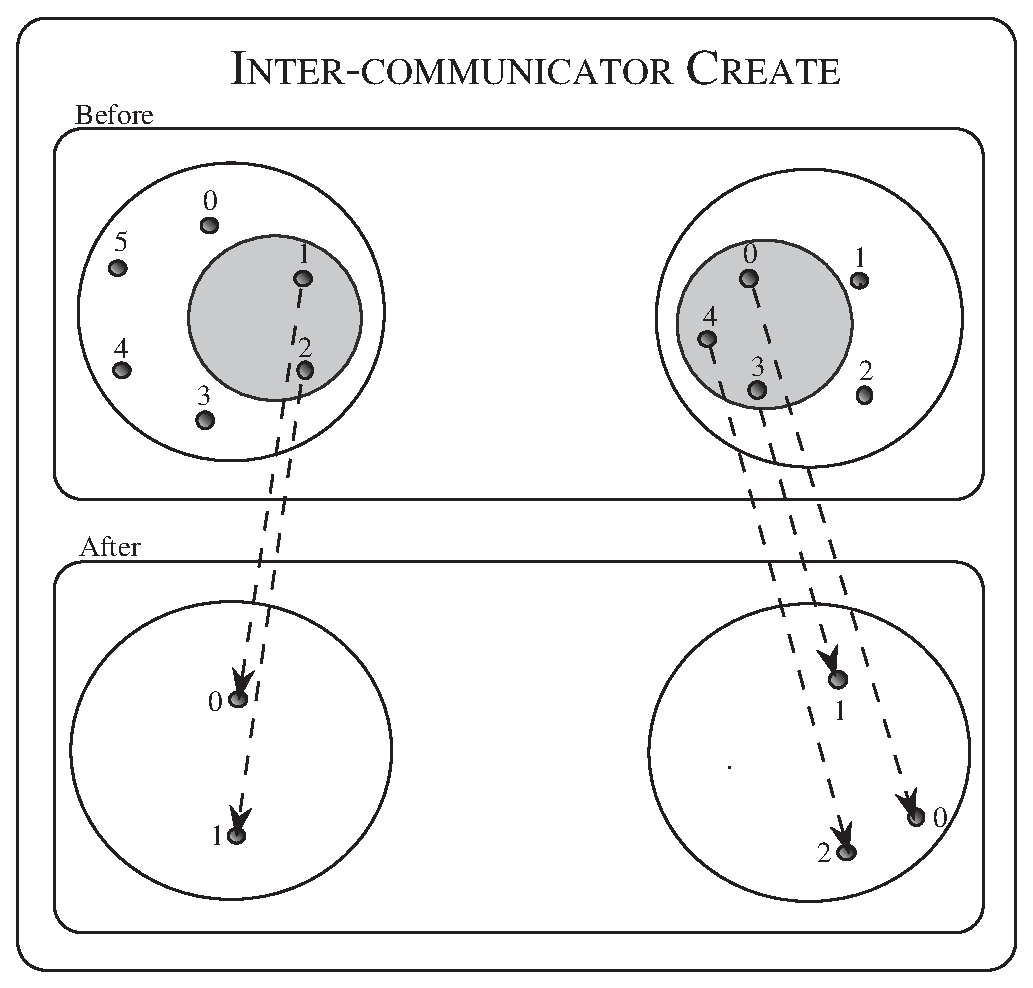
\includegraphics[width=4.0in]{figures/collective-create}}
  \caption[Inter-communicator creation
    using \mpiskipfunc{MPI\_COMM\_CREATE}]{Inter-communicator 
    creation
    using \mpifunc{MPI\_COMM\_CREATE}
extended to inter-communicators. The input groups are those in the grey
circle.}
  \label{fig:collective-create}
\end{figure}

\begin{rationale}
The interface supports the original mechanism from \MPIIDOTI/, which required the same \mpiarg{group} in all
\MPI/ processes of \mpiarg{comm}. It was extended in \MPIIIDOTII/ to allow the use of disjoint subgroups in order to allow
implementations to eliminate unnecessary communication that \mpifunc{MPI\_COMM\_SPLIT} would incur when the user already
knows the membership of the disjoint subgroups.
\end{rationale} 

\begin{rationale}
The requirement that the entire group of \mpiarg{comm} participate in the call
stems from the following considerations:
\begin{itemize}
\item
It allows the implementation to layer \mpifunc{MPI\_COMM\_CREATE} on top of
regular collective communications.
\item
It provides additional safety, in particular in the case where partially
overlapping groups are used to create new communicators.
\item
It permits implementations to
sometimes avoid communication related to
context
creation.
\end{itemize}
\end{rationale}

\begin{users}
\mpifunc{MPI\_COMM\_CREATE} provides a means to subset a group of \MPI/ processes for the
purpose of separate MIMD computation, with separate communication space.
\mpiarg{newcomm}, which emerges from
\mpifunc{MPI\_COMM\_CREATE}, can be used in
subsequent calls to \mpifunc{MPI\_COMM\_CREATE} (or other communicator
constructors) to
further subdivide a computation into
parallel sub-computations. A more general service is provided by
\mpifunc{MPI\_COMM\_SPLIT}, below.
\end{users}

\begin{implementors}
When calling \mpifunc{MPI\_COMM\_DUP}, all \MPI/ processes call with the same \mpiarg{group}
(the \mpiarg{group} associated with the communicator).
When calling \mpifunc{MPI\_COMM\_CREATE}, the \MPI/ processes provide the
same \mpiarg{group} or disjoint subgroups. For both calls, it is theoretically possible
to agree on a group-wide unique context with no communication.
However, local execution of these functions requires
use of a larger context name space and reduces error checking.
Implementations may strike various compromises between these
conflicting goals, such as bulk allocation of multiple contexts in one
collective operation.

Important: If new communicators are created without synchronizing the
\MPI/ processes involved then the communication system
must be able to cope with
messages arriving in a context that has not yet been allocated at the
receiving \MPI/ process.
\end{implementors}

\noindent If \mpiarg{comm} is an
inter-communicator, then the output communicator is also an
inter\hyphen/communicator
where the local group consists only of those \MPI/ processes contained in
\mpiarg{group} (see Figure~\ref{fig:collective-create}). The \mpiarg{group}
argument should only contain those \MPI/ processes in the local group of the input
inter-communicator that are to be a part of \mpiarg{newcomm}.
All \MPI/ processes in the same local group of \mpiarg{comm} must specify the same value for
\mpiarg{group}, i.e., the same members in the same order.
If either
\mpiarg{group} does not specify at least one \MPI/ process in the local group of
the inter-communicator, or if the calling \MPI/ process is not included in the
\mpiarg{group}, \mpiconst{MPI\_COMM\_NULL} is returned.

\begin{rationale}
In the case where either the left or right group is empty, a null communicator
is returned instead of an inter-communicator with \mpiconst{MPI\_GROUP\_EMPTY}
because the side with the empty group must return \mpiconst{MPI\_COMM\_NULL}.
\end{rationale}

\begin{example}
\label{ex:intercomm creation}
\Exindex{C}{Inter-communicator
  creation}{MPI\_Comm\_create,MPI\_Comm\_group,MPI\_Group\_incl,MPI\_Group\_free}%
\exindex{Inter-communicator}%
Inter-communicator creation.\\
The following example illustrates how the first node in the left
side of an inter-communicator could be joined with all members on the
right side of an inter-communicator to form a new
inter-communicator.
%%HEADER
%%LANG: C
%%FRAGMENT
%%SKIPELIPSIS
%%SUBST:/\* I'm on the left side of the inter-communicator \*/:1
%%ENDHEADER
\begin{lstlisting}[language={[MPI]C}]
MPI_Comm  inter_comm, new_inter_comm;
MPI_Group local_group, group;
int       rank = 0; /* rank on left side to include in
                       new inter-comm */

/* Construct the original inter-communicator: "inter_comm" */
...

/* Construct the group of MPI processes to be in new
   inter-communicator */
if (/* I'm on the left side of the inter-communicator */) {
  MPI_Comm_group(inter_comm, &local_group);
  MPI_Group_incl(local_group, 1, &rank, &group);
  MPI_Group_free(&local_group);
}
else
  MPI_Comm_group(inter_comm, &group);

MPI_Comm_create(inter_comm, group, &new_inter_comm);
MPI_Group_free(&group);
\end{lstlisting}
\end{example}

\cdeclmainindex{MPI\_Comm}\cdeclmainindex{TYPE(MPI\_Comm)}
\begin{funcdef}{MPI\_COMM\_CREATE\_GROUP}{(\mbox{comm}, \mbox{group}, \mbox{tag}, \mbox{newcomm})}
\funcarg{\IN}{comm}{intra-communicator (handle)}
\funcarg{\IN}{group}{group, which is a subset of the group of \mpiarg{comm} (handle)}
\funcarg{\IN}{tag}{tag (integer)}
\funcarg{\OUT}{newcomm}{new communicator (handle)}
\end{funcdef}
\mpibindmain{MPI\_Comm\_create\_group}{(\gb{}MPI\_Comm~comm, MPI\_Group~group, int~tag, MPI\_Comm~*newcomm)}
\mpifnewbindmain{MPI\_Comm\_create\_group}{(comm, group, tag, newcomm, ierror) \fargs TYPE(MPI\_Comm), INTENT(IN)\ ::\ \mbox{comm}\fnarg{}TYPE(MPI\_Group), INTENT(IN)\ ::\ \mbox{group}\fnarg{}INTEGER, INTENT(IN)\ ::\ \mbox{tag}\fnarg{}TYPE(MPI\_Comm), INTENT(OUT)\ ::\ \mbox{newcomm}\fnfinalarg{}INTEGER, OPTIONAL, INTENT(OUT)\ ::\ \mbox{ierror}}
\mpifbindmain{MPI\_COMM\_CREATE\_GROUP}{(COMM, GROUP, TAG, NEWCOMM, IERROR) \fargs \fnfinalarg{}INTEGER \mbox{COMM}, \mbox{GROUP}, \mbox{TAG}, \mbox{NEWCOMM}, \mbox{IERROR}}

\mpifunc{MPI\_COMM\_CREATE\_GROUP} is similar to
\mpifunc{MPI\_COMM\_CREATE}; however, \mpifunc{MPI\_COMM\_CREATE} must
be called by all \MPI/ processes in the group of \mpishortarg{comm}, whereas
\mpifunc{MPI\_COMM\_CREATE\_GROUP} must be called by all \MPI/ processes in
\mpishortarg{group}, which is a subgroup of the group of \mpishortarg{comm}. In
addition, \mpifunc{MPI\_COMM\_CREATE\_GROUP} requires that
\mpishortarg{comm} is an
intra-communicator. \mpifunc{MPI\_COMM\_CREATE\_GROUP} returns a new
intra-communicator, \mpiarg{newcomm}, for which the \mpiarg{group}
argument defines the communication group. No cached information
propagates from \mpiarg{comm} to \mpiarg{newcomm} and no virtual topology
information is added to the created communicator. Each \MPI/ process must
provide a \mpiarg{group} argument that is a subgroup of the group associated
with \mpiarg{comm}; this could be \mpiconst{MPI\_GROUP\_EMPTY}. If a
nonempty group is specified, then all \MPI/ processes in that group must
call the function, and each of these \MPI/ processes must provide the same
arguments, including a group that contains the same members with the
same ordering. Otherwise the call is erroneous. If the calling \MPI/ process
is a member of the group given as the \mpiarg{group} argument, then
\mpiarg{newcomm} is a communicator with \mpiarg{group} as its
associated group. If the calling \MPI/ process is not a member of
\mpiarg{group}, e.g., \mpiarg{group} is \mpiconst{MPI\_GROUP\_EMPTY}, then
the call is a local operation and \mpiconst{MPI\_COMM\_NULL} is returned
as \mpiarg{newcomm}.

\begin{rationale}
Functionality similar to \mpifunc{MPI\_COMM\_CREATE\_GROUP} can be
implemented through repeated \mpifunc{MPI\_INTERCOMM\_CREATE} and
\mpifunc{MPI\_INTERCOMM\_MERGE} calls that start with the
\mpiconst{MPI\_COMM\_SELF} communicators at each \MPI/ process in
\mpishortarg{group} and build up an intra-communicator with group
\mpishortarg{group}~\cite{DBLP:conf/pvm/DinanKBHKTV11}. Such an algorithm
requires the creation of many intermediate communicators;
\mpifunc{MPI\_COMM\_CREATE\_GROUP} can provide a more efficient
implementation that avoids this overhead.
\end{rationale}

\begin{users}
An inter-communicator can be created collectively over \MPI/ processes in the union of the local and remote groups by creating the local communicator using \mpifunc{MPI\_COMM\_CREATE\_GROUP} and using that communicator as the local communicator argument to \mpifunc{MPI\_INTERCOMM\_CREATE}.
\end{users}

The \mpiarg{tag} argument does not conflict with tags used in
point-to-point communication and is not permitted to be a wildcard. If
multiple threads at a given \MPI/ process perform concurrent
\mpifunc{MPI\_COMM\_CREATE\_GROUP} operations, the user must
distinguish these operations by providing different \mpiarg{tag} or
\mpiarg{comm} arguments.

\begin{users}
\mpifunc{MPI\_COMM\_CREATE} may provide lower overhead than
\mpifunc{MPI\_COMM\_CREATE\_GROUP} because it can take advantage of
collective communication on \mpiarg{comm} when constructing \mpiarg{newcomm}.
\end{users}

\cdeclindex{MPI\_Comm}%
\begin{funcdef}{MPI\_COMM\_SPLIT}{(\mbox{comm}, \mbox{color}, \mbox{key}, \mbox{newcomm})}
\funcarg{\IN}{comm}{communicator (handle)}
\funcarg{\IN}{color}{control of subset assignment (integer)}
\funcarg{\IN}{key}{control of rank assignment (integer)}
\funcarg{\OUT}{newcomm}{new communicator (handle)}
\end{funcdef}
\mpibindmain{MPI\_Comm\_split}{(\gb{}MPI\_Comm~comm, int~color, int~key, MPI\_Comm~*newcomm)}
\mpifnewbindmain{MPI\_Comm\_split}{(comm, color, key, newcomm, ierror) \fargs TYPE(MPI\_Comm), INTENT(IN)\ ::\ \mbox{comm}\fnarg{}INTEGER, INTENT(IN)\ ::\ \mbox{color}, \mbox{key}\fnarg{}TYPE(MPI\_Comm), INTENT(OUT)\ ::\ \mbox{newcomm}\fnfinalarg{}INTEGER, OPTIONAL, INTENT(OUT)\ ::\ \mbox{ierror}}
\mpifbindmain{MPI\_COMM\_SPLIT}{(COMM, COLOR, KEY, NEWCOMM, IERROR) \fargs \fnfinalarg{}INTEGER \mbox{COMM}, \mbox{COLOR}, \mbox{KEY}, \mbox{NEWCOMM}, \mbox{IERROR}}

\noindent This function partitions the group associated with \mpiarg{comm}
into disjoint subgroups, one for each value of \mpiarg{color}. Each subgroup
contains all \MPI/ processes of the same color. Within each subgroup, the \MPI/ processes
are ranked in the order defined by the value of the argument \mpiarg{key},
with ties broken according to their rank in the old group. A new communicator
is created for each subgroup and returned in \mpiarg{newcomm}. An \MPI/ process may
supply the color value \mpiconst{MPI\_UNDEFINED}, in which case \mpiarg{newcomm}
returns \mpiconst{MPI\_COMM\_NULL}. This is a collective call, but each \MPI/ process
is permitted to provide different values for \mpiarg{color} and \mpiarg{key}.
No cached information propagates from \mpiarg{comm} to \mpiarg{newcomm} and no
virtual topology information is added to the created communicators.

With an intra-communicator \mpiarg{comm}, a call to \mpifunc{MPI\_COMM\_CREATE}\mpicode{(comm, group, newcomm)} is
equivalent to a call to \mpifunc{MPI\_COMM\_SPLIT}\mpicode{(comm, color, key, newcomm)}, where \MPI/ processes
that are members of their \mpiarg{group} argument provide
a \mpiarg{color} argument equal to the number of the \mpiarg{group}
(based on a unique numbering of all disjoint groups) and
a \mpiarg{key} argument equal to their rank in \mpiarg{group}, and
all \MPI/ processes that are not members of their \mpiarg{group} argument provide
a \mpiarg{color} argument equal to \mpiconst{MPI\_UNDEFINED}.
The value of \mpiarg{color} must be
nonnegative or \mpiconst{MPI\_UNDEFINED}.

\begin{users}
This is an extremely powerful mechanism for dividing a single
communicating group of \MPI/ processes into $k$ subgroups, with $k$ chosen
implicitly by the user (by the number of
colors asserted over all the \MPI/ processes). Each resulting communicator will be
nonoverlapping. Such a division could be useful for defining a hierarchy
of computations, such as for multigrid, or linear algebra.
For intra-communicators, \mpifunc{MPI\_COMM\_SPLIT} provides similar capability as \mpifunc{MPI\_COMM\_CREATE}
to split a communicating group into disjoint subgroups. \mpifunc{MPI\_COMM\_SPLIT} is useful
when some \MPI/ processes do not have complete information of the other members in their
group, but all \MPI/ processes know (the color of) the group to which they belong.
In this case, the \MPI/ implementation discovers the other group members via
communication. \mpifunc{MPI\_COMM\_CREATE} is useful when all \MPI/ processes have complete
information of the members of their group. In this case, \MPI/ can avoid the extra
communication required to discover group membership.
\mpifunc{MPI\_COMM\_CREATE\_GROUP} is useful when
all \MPI/ processes in a given group have complete information of the members of
their group and synchronization with \MPI/ processes outside the group can be
avoided.

Multiple calls to \mpifunc{MPI\_COMM\_SPLIT} can be used to overcome the
requirement that any call have no overlap of the resulting communicators (each
\MPI/ process shall belong to only one color per call). In this way, multiple overlapping
communication structures can be created. Creative use of the \mpiarg{color}
and \mpiarg{key} in such splitting operations is encouraged.

Note that, for a fixed color, the keys need not
be unique. It is \mpifunc{MPI\_COMM\_SPLIT}'s responsibility to sort \MPI/ processes
in ascending order according to this key, and to break ties in a consistent
way. If all the keys are specified in the same way, then all the \MPI/ processes
in a given color will have the relative rank order as they did in their
parent group.

\end{users}

\begin{rationale}
\mpiarg{color} is restricted to be nonnegative, so as not to conflict with the value assigned to \mpiconst{MPI\_UNDEFINED}.
\end{rationale}

\begin{figure}[ht]
  \centerline{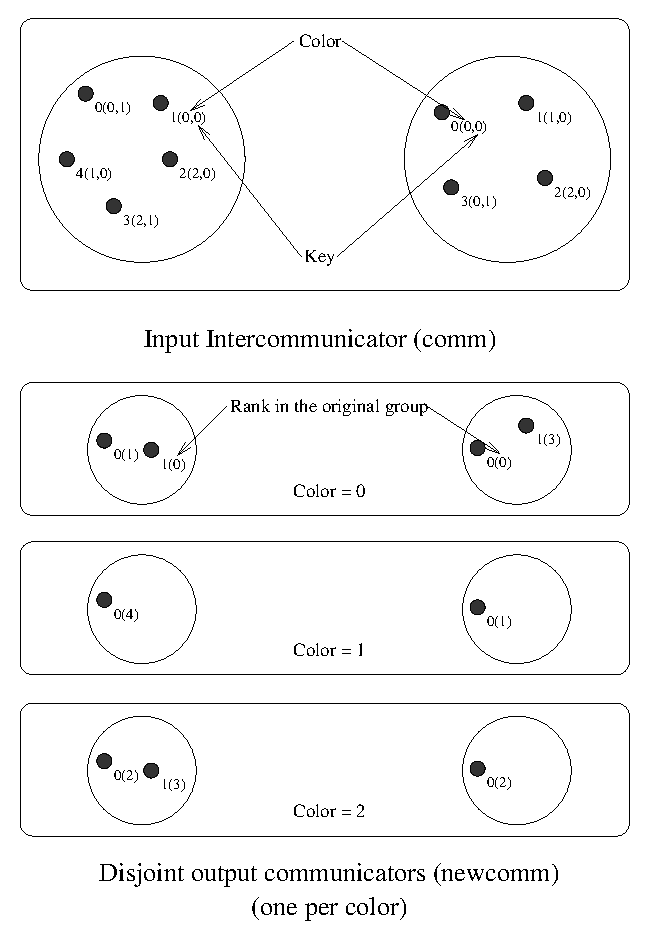
\includegraphics[width=3.5in]{figures/collective-split2}}
  \caption[Inter-communicator construction with \mpiskipfunc{MPI\_COMM\_SPLIT}]{Inter-communicator construction achieved by splitting an
    existing inter-communicator with \mpifunc{MPI\_COMM\_SPLIT}
extended to inter-communicators}
  \label{fig:collective-split}
\end{figure}

\noindent The result of \mpifunc{MPI\_COMM\_SPLIT} on an inter-communicator is that those
\MPI/ processes on the left with the same \mpiarg{color} as those \MPI/ processes on
the right combine to create a new inter-communicator. The \mpiarg{key}
argument describes the relative rank of \MPI/ processes on each side of the
inter-communicator (see Figure~\ref{fig:collective-split}). For those colors
that are specified only on one side of the inter-communicator,
\mpiconst{MPI\_COMM\_NULL} is returned. \mpiconst{MPI\_COMM\_NULL}
is also returned to those \MPI/ processes that specify \mpiconst{MPI\_UNDEFINED}
as the color.
\begin{users}
For inter-communicators, \mpifunc{MPI\_COMM\_SPLIT} is more general than \mpifunc{MPI\_COMM\_CREATE}.
A single call to \mpifunc{MPI\_COMM\_SPLIT} can create a set of disjoint inter-communicators,
while a call to \mpifunc{MPI\_COMM\_CREATE} creates only one.
\end{users}

\begin{example}
\label{ex:para-client-server}
\Exindex{C}{Client-server model}{MPI\_Comm\_split,MPI\_Comm\_remote\_size}%
\exindex{Inter-communicator}%
Parallel client-server model.\\
The following client code illustrates how clients on the left side of an
inter-communicator could be assigned to a single server from a pool of
servers on the right side of an inter-communicator.
%%HEADER
%%LANG: C
%%FRAGMENT
%%SKIPELIPSIS
%%ENDHEADER
\begin{lstlisting}[language={[MPI]C}]
/* Client code */
MPI_Comm  multiple_server_comm;
MPI_Comm  single_server_comm;
int       color, rank, num_servers;

/* Create inter-communicator with clients and servers:
   multiple_server_comm */
...

/* Find out the number of servers available */
MPI_Comm_remote_size(multiple_server_comm, &num_servers);

/* Determine my color */
MPI_Comm_rank(multiple_server_comm, &rank);
color = rank % num_servers;

/* Split the inter-communicator */
MPI_Comm_split(multiple_server_comm, color, rank,
               &single_server_comm);
\end{lstlisting}
\noindent The following is the corresponding server code:
%%HEADER
%%LANG: C
%%FRAGMENT
%%SKIPELIPSIS
%%ENDHEADER
\begin{lstlisting}[language={[MPI]C}]
/* Server code */
MPI_Comm  multiple_client_comm;
MPI_Comm  single_server_comm;
int       rank;

/* Create inter-communicator with clients and servers:
   multiple_client_comm */
...

/* Split the inter-communicator for a single server per group
   of clients */
MPI_Comm_rank(multiple_client_comm, &rank);
MPI_Comm_split(multiple_client_comm, rank, 0,
               &single_server_comm);
\end{lstlisting}
\end{example}

\cdeclindex{MPI\_Comm}%
\begin{funcdef}{MPI\_COMM\_SPLIT\_TYPE}{(\mbox{comm}, \mbox{split\_type}, \mbox{key}, \mbox{info}, \mbox{newcomm})}
\funcarg{\IN}{comm}{communicator (handle)}
\funcarg{\IN}{split\_type}{type of processes to be grouped together (integer)}
\funcarg{\IN}{key}{control of rank assignment (integer)}
\funcarg{\INOUT}{info}{info argument (handle)}
\funcarg{\OUT}{newcomm}{new communicator (handle)}
\end{funcdef}
\mpibindmain{MPI\_Comm\_split\_type}{(\gb{}MPI\_Comm~comm, int~split\_type, int~key, MPI\_Info~info, MPI\_Comm~*newcomm)}
\mpifnewbindmain{MPI\_Comm\_split\_type}{(comm, split\_type, key, info, newcomm, ierror) \fargs TYPE(MPI\_Comm), INTENT(IN)\ ::\ \mbox{comm}\fnarg{}INTEGER, INTENT(IN)\ ::\ \mbox{split\_type}, \mbox{key}\fnarg{}TYPE(MPI\_Info), INTENT(IN)\ ::\ \mbox{info}\fnarg{}TYPE(MPI\_Comm), INTENT(OUT)\ ::\ \mbox{newcomm}\fnfinalarg{}INTEGER, OPTIONAL, INTENT(OUT)\ ::\ \mbox{ierror}}
\mpifbindmain{MPI\_COMM\_SPLIT\_TYPE}{(COMM, SPLIT\_TYPE, KEY, INFO, NEWCOMM, IERROR) \fargs \fnfinalarg{}INTEGER \mbox{COMM}, \mbox{SPLIT\_TYPE}, \mbox{KEY}, \mbox{INFO}, \mbox{NEWCOMM}, \mbox{IERROR}}

\noindent This function partitions the group associated with
\mpiarg{comm} into disjoint subgroups such that each subgroup contains
all \MPI/ processes in the same grouping referred to by \mpiarg{split\_type}.
Within each subgroup, the \MPI/ processes are ranked in the order
defined by the value of the argument \mpiarg{key}, with ties broken
according to their rank in the old group. A new communicator is
created for each subgroup and returned in \mpiarg{newcomm}. This is a
collective call. All \MPI/ processes in the group associated with
\mpiarg{comm} must provide the same \mpiarg{split\_type}, but each
\MPI/ process is permitted to provide different values for \mpiarg{key}.
An exception to this rule is that an \MPI/ process may supply the type
value \mpiconst{MPI\_UNDEFINED}, in which case \mpiconst{MPI\_COMM\_NULL} is
returned in \mpiarg{newcomm} for such \MPI/ process.
No cached information propagates from \mpiarg{comm} to \mpiarg{newcomm} and no
virtual topology information is added to the created communicators.


For \mpiarg{split\_type}, the following values are defined by \MPI/:

\begin{description}

\item[\mpiconstmain{MPI\_COMM\_TYPE\_SHARED}:]all \MPI/ processes in the group of \mpiarg{newcomm}
  are part of the same \mpitermni{shared memory domain}\mpitermindex{shared memory!domain} and
  can create a \mpitermni{shared memory segment}\mpitermindex{shared memory!segment}
  (e.g., with a successful call to \mpifunc{MPI\_WIN\_ALLOCATE\_SHARED}).
  This segment can subsequently be used for load/store accesses by all \MPI/ processes in \mpiarg{newcomm}.

  \begin{users}
    Since the location of some of the \MPI/ processes may change during the application execution,
    the communicators created with the value \mpiconst{MPI\_COMM\_TYPE\_SHARED} before this change may not
    reflect an actual ability to share memory between \MPI/ processes after this change.
  \end{users}

\item[\mpiconstmain{MPI\_COMM\_TYPE\_HW\_GUIDED}:]this
  value specifies that the communicator \mpiarg{comm} is split according to a
  \mpitermdef{hardware resource type} (for example a computing core or an L3 cache)
  specified by the \infokey{mpi\_hw\_resource\_type} info key. Each output communicator
  \mpiarg{newcomm} corresponds to a single instance of the specified hardware resource type.
  The \MPI/ processes in the group associated with the output communicator \mpiarg{newcomm}
  utilize that specific hardware resource type instance, and no other instance of the same
  hardware resource type.

  If an \MPI/ process does not meet the above criteria, then \mpiconst{MPI\_COMM\_NULL} is returned
  in \mpiarg{newcomm} for such \MPI/ process.

  \mpiconst{MPI\_COMM\_NULL} is also returned in \mpiarg{newcomm} in the following cases:
  \begin{itemize}
  \item \mpiconst{MPI\_INFO\_NULL} is provided.
  \item The \mpiarg{info} handle does not include the key \infokey{mpi\_hw\_resource\_type}.
  \item The \MPI/ implementation neither recognizes nor supports the info key \infokey{mpi\_hw\_resource\_type}.
  \item The \MPI/ implementation does not recognize the value associated with the info key \infokey{mpi\_hw\_resource\_type}.
  \end{itemize}

  The \MPI/ implementation will return in the group of the output communicator \mpiarg{newcomm}
  the largest subset of \MPI/ processes that match the splitting criterion.

  The \MPI/ processes in the group associated with \mpiarg{newcomm} are ranked in the order defined by
  the value of the argument \mpiarg{key} with ties broken according to their rank in the group
  associated with \mpiarg{comm}.
  
  \begin{users}
    The set of hardware resources that an \MPI/ process is able to utilize may change during the
    application execution (e.g., because of the relocation of an \MPI/ process), in which case the communicators
    created with the value \mpiconst{MPI\_COMM\_TYPE\_HW\_GUIDED} before this change may not reflect
    the utilization of hardware resources of such \MPI/ process at any time after the communicator creation. 
  \end{users}
  
  The user explicitly constrains with the \mpiarg{info} argument the splitting of the input communicator
  \mpiarg{comm}. To this end, the info key \infokeymain{mpi\_hw\_resource\_type} is reserved and its associated
  value is an implementation-defined string designating the type of the requested hardware. 
  It is strongly recommended that these strings follow the URI format described in~Section~\ref{subsubsec:inquiry-hw-resource-info}
  (e.g., \infovalskip{hwloc://NUMANode}, \infovalskip{hwloc://Package} or \infovalskip{hwloc://L3Cache}).

  The value \infovalmain{mpi\_shared\_memory} is reserved and its use is equivalent to using \mpiconst{MPI\_COMM\_TYPE\_SHARED}
  for the \mpiarg{split\_type} parameter.
  \begin{rationale}
    The value \infoval{mpi\_shared\_memory} is defined in order to ensure consistency between
    the use of \mpiconst{MPI\_COMM\_TYPE\_SHARED} and the use of \mpiconst{MPI\_COMM\_TYPE\_HW\_GUIDED}.
  \end{rationale}

  All \MPI/ processes must provide the same value for the info key \infokey{mpi\_hw\_resource\_type}.

  \begin{example}
  \label{ex:hw-based split}
  \Exindex{C}{Splitting into NUMANode subcommunicators}{MPI\_Comm\_split\_type}%
  Splitting \mpiconst{MPI\_COMM\_WORLD} into NUMANode subcommunicators.
%%HEADER
%%LANG: C
%%FRAGMENT
%%ENDHEADER
\begin{lstlisting}[language={[MPI]C}]
MPI_Info info;
MPI_Comm hwcomm;
int      rank;

MPI_Comm_rank(MPI_COMM_WORLD, &rank);
MPI_Info_create(&info);
MPI_Info_set(info, "mpi_hw_resource_type", "hwloc://NUMANode");
MPI_Comm_split_type(MPI_COMM_WORLD,
                    MPI_COMM_TYPE_HW_GUIDED,
                    rank, info, &hwcomm);
\end{lstlisting}
\end{example}

\item[\mpiconstmain{MPI\_COMM\_TYPE\_RESOURCE\_GUIDED}:]this
  value specifies that the communicator \mpiarg{comm} is split according to a
  \mpitermdef{hardware resource type} (for example a computing core or an L3 cache)
  specified by the \infokey{mpi\_hw\_resource\_type} info key or to a \mpitermdef{logical resource type}
  (for example a process set name, see Section~\ref{subsec:process_sets})
  specified by the \infokey{mpi\_pset\_name} info key.

  Each output communicator \mpiarg{newcomm} corresponds to a single instance of the specified resource type.
  The \MPI/ processes in the group associated with the output communicator \mpiarg{newcomm}
  utilize that specific resource type instance, and no other instance of the same resource type.

  If an \MPI/ process does not meet the above criteria, then \mpiconst{MPI\_COMM\_NULL} is returned
  in \mpiarg{newcomm} for such process.

  \mpiconst{MPI\_COMM\_NULL} is also returned in \mpiarg{newcomm} in the following cases:
  \begin{itemize}
  \item \mpiconst{MPI\_INFO\_NULL} is provided.
  \item The \mpiarg{info} handle includes neither the key \infokey{mpi\_hw\_resource\_type} nor the key \infokey{mpi\_pset\_name}.
  \item The \MPI/ implementation neither recognizes nor supports the info keys \infokey{mpi\_hw\_resource\_type} and \infokey{mpi\_pset\_name}.
  \item The \MPI/ implementation does not recognize the value associated with the info key \infokey{mpi\_hw\_resource\_type} or \infokey{mpi\_pset\_name}.
  \end{itemize}

  The \MPI/ implementation will return in the group of the output communicator \mpiarg{newcomm}
  the largest subset of \MPI/ processes that match the splitting criterion.

  \begin{users}
    The set of resources that an \MPI/ process is able to utilize may change during the
    application execution (e.g., because of the relocation of an \MPI/ process), in which case the communicators
    created with the value \mpiconst{MPI\_COMM\_TYPE\_RESOURCE\_GUIDED} before this change may not reflect
    the utilization of resources of such process at any time after the communicator creation.
  \end{users}

  The user explicitly constrains with the \mpiarg{info} argument the splitting of the input communicator
  \mpiarg{comm}. To this end, the following info keys are reserved and their associated values
  are implementation-defined strings designating the type of the requested resource. Only one of these info
  keys can be used in \mpiarg{info} at a time in a call to \mpifunc{MPI\_COMM\_SPLIT\_TYPE}; use of more than
  one info key is erroneous.

  \begin{description}
  \item \infokey{mpi\_hw\_resource\_type} is used to specify the type of a requested hardware resource (e.g., \infovalskip{hwloc://NUMANode},
    \infovalskip{hwloc://Package} or \infovalskip{hwloc://L3Cache}). The value \infoval{mpi\_shared\_memory} is reserved and its use is equivalent
    to using \mpiconst{MPI\_COMM\_TYPE\_SHARED} for the \mpiarg{split\_type} parameter.
    \begin{rationale}
      The value \infoval{mpi\_shared\_memory} is defined in order to ensure consistency between
      the use of \mpiconst{MPI\_COMM\_TYPE\_SHARED} and the use of \mpiconst{MPI\_COMM\_TYPE\_RESOURCE\_GUIDED}.
    \end{rationale}

    All \MPI/ processes in the group of the input communicator \mpiarg{comm} must provide the same info key to perform the splitting action.
    All \MPI/ processes in the group of the input communicator \mpiarg{comm} must provide the same value for the info key \infokey{mpi\_hw\_resource\_type}.

  \item \infokeymain{mpi\_pset\_name} is used to specify the type of a requested logical resource through the utilization
    of a process set name (e.g., \infovalskip{app://ocean} or \infovalskip{app://atmos}). This process set name must be valid in the session
    from which the input communicator \mpiarg{comm} is derived. If this input communicator is not derived from a session,
    then \mpiconst{MPI\_COMM\_NULL} is returned in \mpiarg{newcomm}.

    All \MPI/ processes that are both in the group of the input communicator \mpiarg{comm} and in the process set identified by the given process set name
    must provide the same info key to perform the splitting action.
    All \MPI/ processes that are both in the group of the input communicator \mpiarg{comm} and in the process set identified by the given process set name
    must provide the same value for the info key \infokey{mpi\_pset\_name}.
  \end{description}
  
\begin{example}
\label{ex:hw-based split2}
\exindex{MPI\_Comm\_split\_type}%
Splitting \mpiconst{MPI\_COMM\_WORLD} into NUMANode subcommunicators.
%%HEADER
%%LANG: C
%%FRAGMENT
%%ENDHEADER
\begin{lstlisting}[language={[MPI]C}]
    MPI_Info info;
    MPI_Comm hwcomm;
    int      rank;

    MPI_Comm_rank(MPI_COMM_WORLD, &rank);
    MPI_Info_create(&info);
    MPI_Info_set(info, "mpi_hw_resource_type", "hwloc://NUMANode");
    MPI_Comm_split_type(MPI_COMM_WORLD,
                        MPI_COMM_TYPE_RESOURCE_GUIDED,
                        rank, info, &hwcomm);
\end{lstlisting}
\end{example}


\item[\mpiconstmain{MPI\_COMM\_TYPE\_HW\_UNGUIDED}:]the group of \MPI/ processes associated
  with \mpiarg{newcomm} must be a \emph{strict} subset of the group associated with \mpiarg{comm} and
  each \mpiarg{newcomm} corresponds to a single instance of a \mpitermdef{hardware resource type}
  (for example a computing core or an L3 cache).

  All \MPI/ processes in the group associated with \mpiarg{comm} that utilize that specific hardware resource
type instance---and no other instance of the same hardware resource type---are included in the group of
  \mpiarg{newcomm}.
  
  If a given \MPI/ process cannot be a member of a communicator that forms such a strict subset,
  or does not meet the above criteria, then \mpiconst{MPI\_COMM\_NULL} is returned in \mpiarg{newcomm}
  for this process.

  \begin{implementors}
    In a high-quality \MPI/ implementation, the number of different new valid communicators
    \mpiarg{newcomm} produced by this splitting operation should be minimal unless the user
    provides a key/value pair that modifies this behavior. The sets of hardware resource types
    used for the splitting operation are implementation-dependent, but should reflect the hardware
    of the actual system on which the application is currently executing.
  \end{implementors}

  \begin{rationale}
    If the hardware resources are hierarchically organized, calling this routine several times
    using as its input communicator \mpiarg{comm} the output communicator \mpiarg{newcomm} of the
    previous call creates a sequence of \mpiarg{newcomm} communicators in each \MPI/ process, which
    exposes a hierarchical view of the hardware platform, as shown in Example~\ref{ex:recursive-split}.
    This sequence of returned \mpiarg{newcomm} communicators may differ from the sets of hardware
    resource types, as shown in the second splitting operation in Figure~\ref{fig:recursive-split}.
  \end{rationale}

  \begin{users}
    Each output communicator \mpiarg{newcomm} can represent a different hardware resource type
    (see Figure~\ref{fig:recursive-split} for an example). The set of hardware resources
    an \MPI/ process utilizes may change during the application execution (e.g., because
    of \MPI/ process relocation), in which case the communicators created with the value
    \mpiconst{MPI\_COMM\_TYPE\_HW\_UNGUIDED} before this change may not reflect the utilization of
    hardware resources for such \MPI/ process at any time after the communicator creation.
  \end{users}
  
  \begin{figure}[htpb]
    \centerline{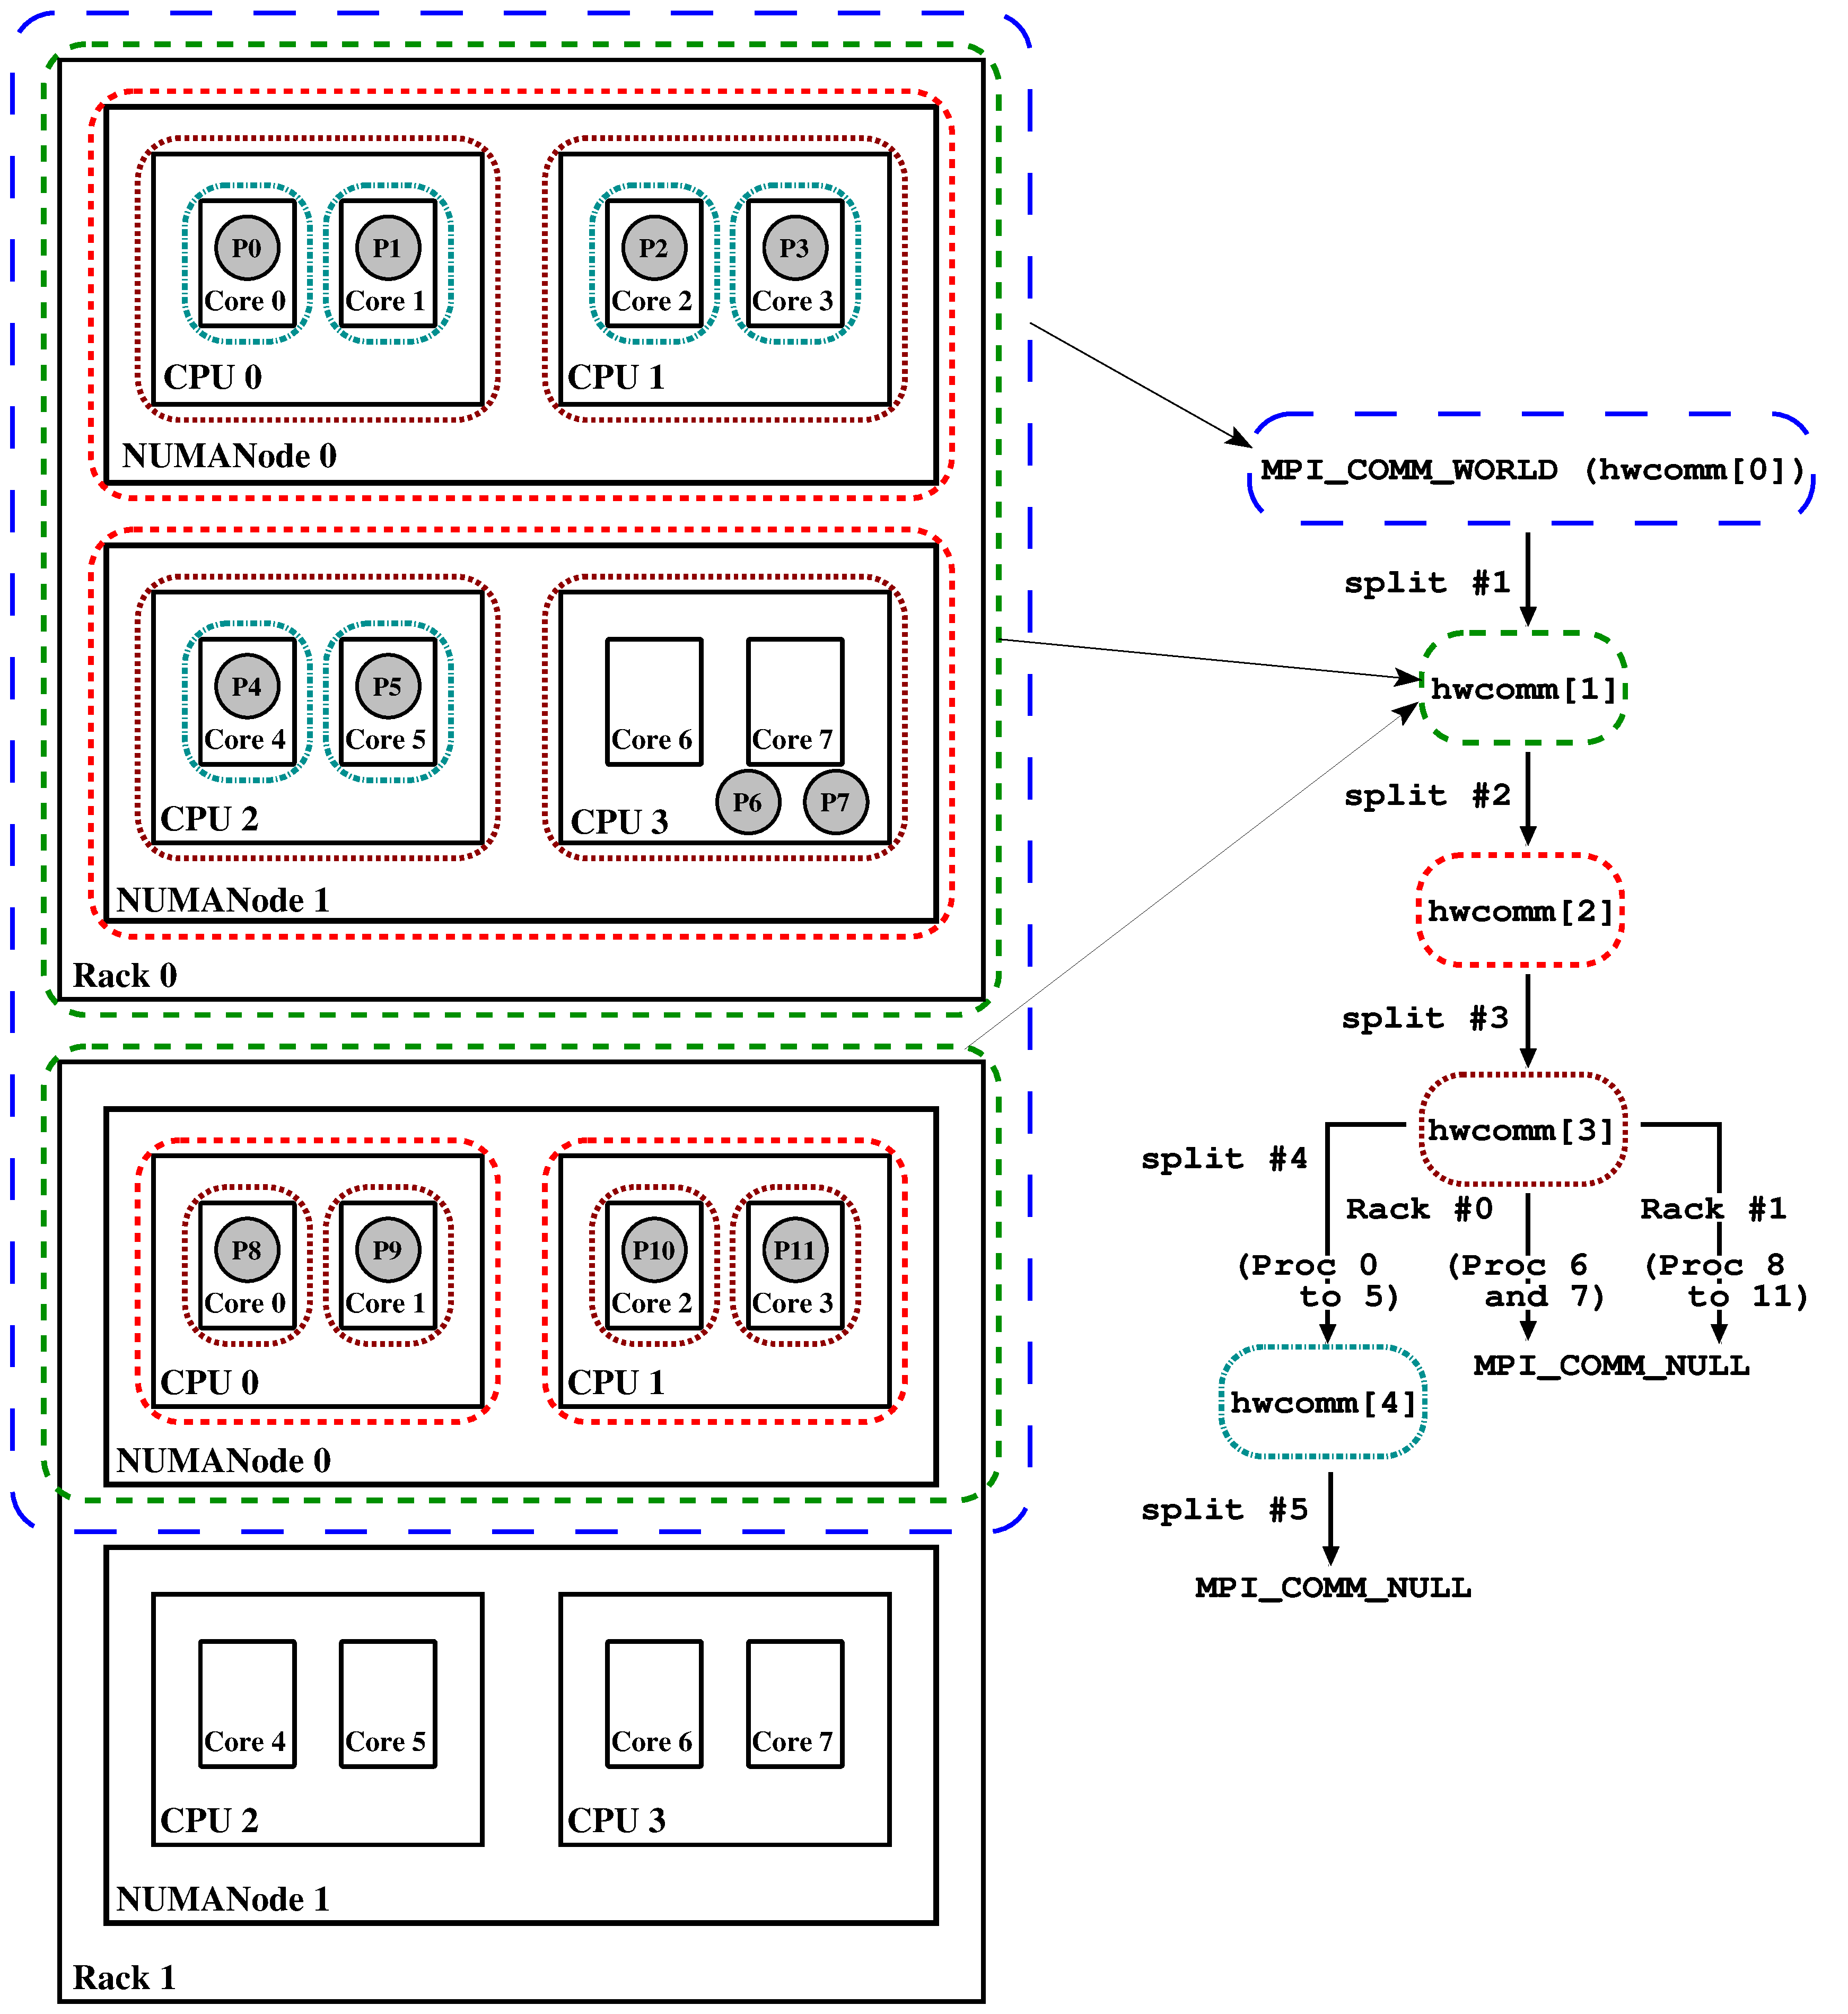
\includegraphics[width=6.0in]{figures/recursive_split}}
    \caption[Recursive communicator creation with \mpiskipfunc{MPI\_COMM\_SPLIT\_TYPE}]{Recursive splitting of
      \mpiconst{MPI\_COMM\_WORLD} with \mpifunc{MPI\_COMM\_SPLIT\_TYPE} and \mpiconst{MPI\_COMM\_TYPE\_HW\_UNGUIDED}.
      Dashed lines represent communicators whilst solid lines represent hardware resources. \MPI/ processes (P0 to
      P11) utilize exclusively their respective core, except for P6 and P7, which utilize
      CPU \#3 of Rack \#0 and can therefore use Cores \#6 and \#7 indifferently. The second splitting operation
      yields two subcommunicators corresponding to \mbox{NUMANodes} in Rack \#0 and to CPUs in Rack \#1 because Rack \#1
      features only one \mbox{NUMANode}, which corresponds to the whole portion of the Rack that is included in
      \mpiconst{MPI\_COMM\_WORLD} and \code{hwcomm[1]}.
      For the first splitting operation, the hardware resource type returned in the info argument is \infovalskip{Rack}
      on the \MPI/ processes on Rack \#0, whereas on Rack \#1, it can be either \infovalskip{Rack} or \infovalskip{NUMANode}.
    }
    \label{fig:recursive-split}
  \end{figure}
  
  If a valid info handle is provided as an argument, the \MPI/ implementation sets the info key
  \infokey{mpi\_hw\_resource\_type} for each \MPI/ process in the group associated with a returned
  \mpiarg{newcomm} communicator and the info key value is an implementation-defined string that
  indicates the hardware resource type represented by \mpiarg{newcomm}. The same hardware resource
  type must be set in all \MPI/ processes in the group associated with \mpiarg{newcomm}.
      
  \begin{example}
  \label{ex:recursive-split}
  \Exindex{C}{Recursive splitting of COMM\_WORLD}{MPI\_Comm\_split\_type}%
  Recursive splitting of \mpiconst{MPI\_COMM\_WORLD}.
%%HEADER
%%LANG: C
%%FRAGMENT
%%ENDHEADER
\begin{lstlisting}[language={[MPI]C}]
#define MAX_NUM_LEVELS 32

MPI_Comm hwcomm[MAX_NUM_LEVELS];
int      rank, level_num = 0;

hwcomm[level_num] = MPI_COMM_WORLD;

while((hwcomm[level_num] != MPI_COMM_NULL) 
      && (level_num < MAX_NUM_LEVELS-1)){
  MPI_Comm_rank(hwcomm[level_num],&rank);
  MPI_Comm_split_type(hwcomm[level_num],
                      MPI_COMM_TYPE_HW_UNGUIDED,
                      rank,
                      MPI_INFO_NULL,
                      &hwcomm[level_num+1]);
  level_num++;
}
\end{lstlisting}
  \end{example}
 
\end{description}

\begin{implementors}
  Implementations can define their own \mpiarg{split\_type} values, or use the \mpiarg{info} argument, to
  assist in creating communicators that help expose platform-specific information to the application.
  The concept of hardware-based communicators was first described by Tr{\"a}ff~\cite{Traff03:archaware} for SMP systems.
  Guided and unguided modes description as well as an implementation path are introduced by
  Goglin et al.~\cite{hsplit18}.
\end{implementors}

\begin{funcdef}{MPI\_COMM\_CREATE\_FROM\_GROUP}{(\mbox{group}, \mbox{stringtag}, \mbox{info}, \mbox{errhandler}, \mbox{newcomm})}
\funcarg{\IN}{group}{group (handle)}
\funcarg{\IN}{stringtag}{unique identifier for this operation (string)}
\funcarg{\IN}{info}{info object (handle)}
\funcarg{\IN}{errhandler}{error handler to be attached to new intra-communicator (handle)}
\funcarg{\OUT}{newcomm}{new communicator (handle)}
\end{funcdef}
\mpibindmain{MPI\_Comm\_create\_from\_group}{(\gb{}MPI\_Group~group, const~char~*stringtag, MPI\_Info~info, MPI\_Errhandler~errhandler, MPI\_Comm~*newcomm)}
\mpifnewbindmain{MPI\_Comm\_create\_from\_group}{(group, stringtag, info, errhandler, newcomm, ierror) \fargs TYPE(MPI\_Group), INTENT(IN)\ ::\ \mbox{group}\fnarg{}CHARACTER(LEN=*), INTENT(IN)\ ::\ \mbox{stringtag}\fnarg{}TYPE(MPI\_Info), INTENT(IN)\ ::\ \mbox{info}\fnarg{}TYPE(MPI\_Errhandler), INTENT(IN)\ ::\ \mbox{errhandler}\fnarg{}TYPE(MPI\_Comm), INTENT(OUT)\ ::\ \mbox{newcomm}\fnfinalarg{}INTEGER, OPTIONAL, INTENT(OUT)\ ::\ \mbox{ierror}}
\mpifbindmain{MPI\_COMM\_CREATE\_FROM\_GROUP}{(GROUP, STRINGTAG, INFO, ERRHANDLER, NEWCOMM, IERROR) \fargs INTEGER \mbox{GROUP}, \mbox{INFO}, \mbox{ERRHANDLER}, \mbox{NEWCOMM}, \mbox{IERROR}\fnfinalarg{}CHARACTER*(*) \mbox{STRINGTAG}}

\mpifunc{MPI\_COMM\_CREATE\_FROM\_GROUP} is similar to
\mpifunc{MPI\_COMM\_CREATE\_GROUP}, except that the set of \MPI/ processes
involved in the creation of the new intra-communicator is specified by a
\mpiarg{group} argument, rather than the group associated with a pre-existing communicator.
If a nonempty \mpiarg{group} is specified, then
all \MPI/ processes in that group must call the function and
each of these \MPI/ processes must provide the same arguments,
including a group that contains the same members with the same ordering,
and identical \mpiarg{stringtag} value.
In the event that \mpiconst{MPI\_GROUP\_EMPTY} is supplied as the \mpiarg{group} argument, then
the call is a local operation and \mpiconst{MPI\_COMM\_NULL} is returned as \mpiarg{newcomm}.
The \mpiarg{stringtag} argument is analogous to the \mpiarg{tag} used for \mpifunc{MPI\_COMM\_CREATE\_GROUP}.
If multiple threads at a given \MPI/ process perform concurrent
\mpifunc{MPI\_COMM\_CREATE\_FROM\_GROUP} operations, the user must
distinguish these operations by providing different \mpiarg{stringtag} arguments.
The \mpiarg{stringtag} shall not exceed \mpiconstmain{MPI\_MAX\_STRINGTAG\_LEN}  characters in length.
For C, this includes space for a null terminating character.
\mpiconst{MPI\_MAX\_STRINGTAG\_LEN} shall have a value of at least 63.

The \mpiarg{errhandler} argument specifies an
error handler to be attached to the new intra-communicator.
Section~\ref{sec:errorhandler} specifies the error handler to be invoked if
an error is encountered during the invocation of \mpifunc{MPI\_COMM\_CREATE\_FROM\_GROUP}.

The \mpiarg{info} argument provides hints and assertions,
possibly \MPI/ implementation dependent,
which indicate desired characteristics and guide communicator creation.

\begin{users}
The \mpiarg{stringtag} argument is used to distinguish concurrent communicator construction operations
issued by different entities. As such, it is important to ensure that this argument is unique
for each concurrent call to \mpifunc{MPI\_COMM\_CREATE\_FROM\_GROUP}.
Reverse domain name notation convention~\cite{reverseDNS} is one approach to constructing unique \mpiarg{stringtag} arguments.
See also example~\ref{exa:session1}.
\end{users}

\subsection{Communicator Destructors}
\label{subsec:context-intracomdest}

\cdeclindex{MPI\_Comm}%
\begin{funcdef}{MPI\_COMM\_FREE}{(\mbox{comm})}
\funcarg{\INOUT}{comm}{communicator to be destroyed (handle)}
\end{funcdef}
\mpibindmain{MPI\_Comm\_free}{(\gb{}MPI\_Comm~*comm)}
\mpifnewbindmain{MPI\_Comm\_free}{(comm, ierror) \fargs TYPE(MPI\_Comm), INTENT(INOUT)\ ::\ \mbox{comm}\fnfinalarg{}INTEGER, OPTIONAL, INTENT(OUT)\ ::\ \mbox{ierror}}
\mpifbindmain{MPI\_COMM\_FREE}{(COMM, IERROR) \fargs \fnfinalarg{}INTEGER \mbox{COMM}, \mbox{IERROR}}

This collective operation marks the communication object for
deallocation.
Any operations that use the communicator \mpiarg{comm} (whether active or inactive at
the time of this procedure call) will continue to work;
the object is actually deallocated only if there are no other active references to it. 
The handle is set to \mpiconst{MPI\_COMM\_NULL} in the calling \MPI/ process.
This call applies to intra- and inter-communicators. The delete callback
functions for all cached attributes (see Section~\ref{sec:caching}) are
called in arbitrary order.

\begin{implementors}
Though collective, it is anticipated that this operation will normally
be implemented to be local, though
a 
debugging version of an \MPI/ library might
choose to synchronize.
\end{implementors}

\subsection{Communicator Info}
\label{sec:comm-info}

Hints specified via info (see Chapter~\ref{chap:misc-2}) allow a user
to provide information to direct optimization. Providing hints may
enable an implementation to deliver increased performance or minimize
use of system resources. As described in \sectionref{subsec:info},
an implementation is free to ignore all hints; however, applications
must comply with any info hints they provide that are used by the \MPI/
implementation (i.e., are returned by a call to
\mpifunc{MPI\_COMM\_GET\_INFO}) and that place a restriction on the
behavior of the application.
Hints are specified on a per communicator basis, in
\mpifunc{MPI\_COMM\_DUP\_WITH\_INFO},
\mpifunc{MPI\_COMM\_IDUP\_WITH\_INFO},
\mpifunc{MPI\_COMM\_SET\_INFO},
\mpifunc{MPI\_COMM\_SPLIT\_TYPE},
\mpifunc{MPI\_DIST\_GRAPH\_CREATE}, and
\mpifunc{MPI\_DIST\_GRAPH\_CREATE\_ADJACENT},
via the opaque info object. When
an info object that specifies a subset of valid hints is passed to
\mpifunc{MPI\_COMM\_SET\_INFO}, there will be no effect on previously
set or defaulted hints that the info does not specify.

\begin{implementors}
It may happen that a program is coded with hints for one system, and
later executes on another system that does not support these hints. In
general, unsupported hints should simply be ignored. Needless to say,
no hint can be mandatory. However, for each hint used by a specific
implementation, a default value must be provided when the user does
not specify a value for this hint.
\end{implementors}

\begin{users}
Some optimizations may only be possible when all \MPI/ processes in the group of the
communicator provide a given info key with the same value.
\end{users}

Info hints are not propagated by \MPI/ from one communicator to another.
The following info keys are valid for all communicators.

\begin{description}

\item[\infokeymain{mpi\_assert\_no\_any\_tag} (boolean, default: \infoval{false}):]
If set to \infoval{true}, then the implementation may assume that the \MPI/ process will not
use the \mpiconst{MPI\_ANY\_TAG} wildcard on the given communicator.

\item[\infokeymain{mpi\_assert\_no\_any\_source} (boolean, default: \infoval{false}):]
If set to \infoval{true}, then the implementation may assume that the \MPI/ process will not
use the \mpiconst{MPI\_ANY\_SOURCE} wildcard on the given communicator.

\item[\infokeymain{mpi\_assert\_exact\_length} (boolean, default: \infoval{false}):]
If set to \infoval{true}, then the implementation may assume that the lengths of messages
received by the \MPI/ process are equal to the lengths of the corresponding receive
buffers, for point-to-point communication operations on the given communicator.

\item[\infokeymain{mpi\_assert\_allow\_overtaking} (boolean, default: \infoval{false}):]
If set to \infoval{true}, then the implementation may assume that point-to-point
communications on the given communicator do not rely on the nonovertaking rule
specified in Section~\ref{sec:pt2pt-semantics}. In other words, the application
asserts that send operations are not required to be matched at the receiver in
the order in which the send operations were posted by the sender, and
receive operations are not required to be matched in the order in which they
were posted by the receiver.

\begin{users}
Use of the \infokey{mpi\_assert\_allow\_overtaking} info key can result in
nondeterminism in the message matching order.
\end{users}

\label{page:comm-info-strict-pcoll-ordering}
\item[\infokeymain{mpi\_assert\_strict\_persistent\_collective\_ordering} (boolean, default: \infoval{false}):]
If set to \infoval{true}, then the implementation may assume that all the persistent collective
operations are started in the same order across all \MPI/ processes in the group of the communicator.
It is required that if this assertion is made on one member of the
communicator's group, then it must be made on all members of that
communicator's group with the same value.

\begin{users}
Use of the \infokey{mpi\_assert\_strict\_persistent\_collective\_ordering} may
be needed because some optimizations may only be possible on certain
systems when strict collective ordering is asserted for the
underlying communicator of a persistent collective operation.
\end{users}

\item[\infokey{mpi\_assert\_memory\_alloc\_kinds} (string, not set by default):]
If set, the implementation may assume that the memory for all
communication buffers passed to \MPI/ operations performed by the calling \MPI/
process on the given communicator will use only the memory allocation kinds
listed in the value string. See Section~\ref{subsec:mem_alloc_kinds}.

\end{description}

\cdeclindex{MPI\_Comm}%
\begin{funcdef}{MPI\_COMM\_SET\_INFO}{(\mbox{comm}, \mbox{info})}
\funcarg{\INOUT}{comm}{communicator (handle)}
\funcarg{\IN}{info}{info object (handle)}
\end{funcdef}
\mpibindmain{MPI\_Comm\_set\_info}{(\gb{}MPI\_Comm~comm, MPI\_Info~info)}
\mpifnewbindmain{MPI\_Comm\_set\_info}{(comm, info, ierror) \fargs TYPE(MPI\_Comm), INTENT(IN)\ ::\ \mbox{comm}\fnarg{}TYPE(MPI\_Info), INTENT(IN)\ ::\ \mbox{info}\fnfinalarg{}INTEGER, OPTIONAL, INTENT(OUT)\ ::\ \mbox{ierror}}
\mpifbindmain{MPI\_COMM\_SET\_INFO}{(COMM, INFO, IERROR) \fargs \fnfinalarg{}INTEGER \mbox{COMM}, \mbox{INFO}, \mbox{IERROR}}

\mpifunc{MPI\_COMM\_SET\_INFO} updates the hints of the communicator
associated with \mpiarg{comm} using the hints provided in \mpiarg{info}.
This operation has no effect on previously set or defaulted hints that
are not specified by \mpiarg{info}. It also has no effect on previously
set or defaulted hints that are specified by \mpiarg{info}, but are
ignored by the \MPI/ implementation in this call to
\mpifunc{MPI\_COMM\_SET\_INFO}.
\mpifunc{MPI\_COMM\_SET\_INFO} is a collective
routine. The info object may be different on each \MPI/ process, but any
info entries that an implementation requires to be the same on all
\MPI/ processes must appear with the same value in each \MPI/ process's info
object.

\begin{users}
Some info items that an implementation can use when it creates a
communicator cannot easily be changed once the communicator has been
created. Thus, an implementation may ignore hints issued in this call
that it would have accepted in a creation call.
An implementation may also be unable to update certain info hints in a call to \mpifunc{MPI\_COMM\_SET\_INFO}.
\mpifunc{MPI\_COMM\_GET\_INFO} can be used to determine whether updates
to existing info hints were ignored by the implementation.
\end{users}

\begin{users}
Setting info hints on the predefined communicators \mpiconst{MPI\_COMM\_WORLD}
and \mpiconst{MPI\_COMM\_SELF} may have unintended effects, as changes to these
global objects may affect all components of the application, including
libraries and tools.
Users must ensure that all components of the application that use a given
communicator, including libraries and tools, can comply with any info hints
associated with that communicator.
\end{users}

\cdeclindex{MPI\_Comm}%
\begin{funcdef}{MPI\_COMM\_GET\_INFO}{(\mbox{comm}, \mbox{info\_used})}
\funcarg{\IN}{comm}{communicator object (handle)}
\funcarg{\OUT}{info\_used}{new info object (handle)}
\end{funcdef}
\mpibindmain{MPI\_Comm\_get\_info}{(\gb{}MPI\_Comm~comm, MPI\_Info~*info\_used)}
\mpifnewbindmain{MPI\_Comm\_get\_info}{(comm, info\_used, ierror) \fargs TYPE(MPI\_Comm), INTENT(IN)\ ::\ \mbox{comm}\fnarg{}TYPE(MPI\_Info), INTENT(OUT)\ ::\ \mbox{info\_used}\fnfinalarg{}INTEGER, OPTIONAL, INTENT(OUT)\ ::\ \mbox{ierror}}
\mpifbindmain{MPI\_COMM\_GET\_INFO}{(COMM, INFO\_USED, IERROR) \fargs \fnfinalarg{}INTEGER \mbox{COMM}, \mbox{INFO\_USED}, \mbox{IERROR}}

\mpifunc{MPI\_COMM\_GET\_INFO} returns a new info object containing
the hints of the communicator associated with \mpiarg{comm}.
The current setting of all hints related to this communicator is
returned in \mpiarg{info\_used}. An \MPI/ implementation is required to
return all hints that are supported by the implementation and have
default values specified; any user-supplied hints that were not ignored
by the implementation; and any additional hints that were set by
the implementation.
If no such hints
exist, a handle to a newly created info object is returned that
contains no key/value pair. The user is responsible for freeing
\mpiarg{info\_used} via \mpifunc{MPI\_INFO\_FREE}.

%----------------------------------------------------------------------

\section{Motivating Examples}
\label{sec:context:examples}

\subsection{Current Practice \#1}

\begin{example}
\label{ex:context-ex1}
\Exindex{C}{Parallel output of a message}{}
\noindent Parallel output of a message
%%HEADER
%%LANG: C
%%SKIPELIPSIS
%%DECL: int keyval1, keyval2, keyval3;
%%ENDHEADER
\begin{lstlisting}[language={[MPI]C}]
int main(int argc, char *argv[])
{
  int me, size;
  ...
  MPI_Init(&argc, &argv);
  MPI_Comm_rank(MPI_COMM_WORLD, &me);
  MPI_Comm_size(MPI_COMM_WORLD, &size);

  printf("MPI process %d size %d\n", me, size);
  ...
  MPI_Finalize();
  return 0;
}
\end{lstlisting}
Example~\ref{ex:context-ex1} is a do-nothing program that initializes itself,
and refers to the ``all'' communicator, and prints a message. It
terminates itself too. This example does not imply that \MPI/
supports \code{printf}-like communication itself.
\end{example}

\begin{example}
\noindent Message exchange (supposing that \code{size} is even)
\label{ex:context-mexchange}
\Exindex{C}{Message exchange}{}
%%HEADER
%%LANG: C
%%SUBST:\.\.\., me \+ 1:MPI_BOTTOM,0,MPI_INT, me + 1
%%SUBST:\.\.\., me - 1:MPI_BOTTOM,0,MPI_INT, me - 1
%%DECL: MPI_Status status;
%%SKIPELIPSIS
%%ENDHEADER
\begin{lstlisting}[language={[MPI]C}]
int main(int argc, char *argv[])
{
   int me, size;
   int SOME_TAG = 0;
   ...
   MPI_Init(&argc, &argv);

   MPI_Comm_rank(MPI_COMM_WORLD, &me);   /* local */
   MPI_Comm_size(MPI_COMM_WORLD, &size); /* local */

   if((me % 2) == 0)
   {
      /* send unless highest-numbered MPI process */
      if((me + 1) < size)
         MPI_Send(..., me + 1, SOME_TAG, MPI_COMM_WORLD);
   }
   else
      MPI_Recv(..., me - 1, SOME_TAG, MPI_COMM_WORLD, &status);

   ...
   MPI_Finalize();
   return 0;
}
\end{lstlisting}
Example~\ref{ex:context-mexchange} schematically illustrates
message exchanges between ``even'' and ``odd'' \MPI/ processes in the ``all''
communicator.
\end{example}

\subsection{Current Practice \#2}
\begin{example}
\label{ex:context-ex2}
\Exindex{C}{Collective communication}{MPI\_Bcast}
%%HEADER
%%LANG: C
%%SKIPELIPSIS
%%ENDHEADER
\begin{lstlisting}[language={[MPI]C}]
int main(int argc, char *argv[])
{
  int me, count;
  void *data;
  ...

  MPI_Init(&argc, &argv);
  MPI_Comm_rank(MPI_COMM_WORLD, &me);

  if(me == 0)
  {
      /* get input, create buffer ``data'' */
      ...
  }

  MPI_Bcast(data, count, MPI_BYTE, 0, MPI_COMM_WORLD);

  ...
  MPI_Finalize();
  return 0;
}
\end{lstlisting}
Example~\ref{ex:context-ex2} illustrates the use of a collective communication.
\end{example}


\subsection{(Approximate) Current Practice \#3}
\begin{example}
\label{ex:context-ex3}
\Exindex{C}{Using Group\_excl}{MPI\_Comm\_create,MPI\_Group\_excl,MPI\_Group\_free}%
%%HEADER
%%LANG: C
%%SKIPELIPSIS
%%ENDHEADER
\begin{lstlisting}[language={[MPI]C},basicstyle=\lstsmall]
int main(int argc, char *argv[])
{
  int me, count, count2;
  void *send_buf, *recv_buf, *send_buf2, *recv_buf2;
  MPI_Group group_world, grprem;
  MPI_Comm commWorker;
  static int ranks[] = {0};
  ...
  MPI_Init(&argc, &argv);
  MPI_Comm_group(MPI_COMM_WORLD, &group_world);
  MPI_Comm_rank(MPI_COMM_WORLD, &me);  /* local */

  MPI_Group_excl(group_world, 1, ranks, &grprem);  /* local */
  MPI_Comm_create(MPI_COMM_WORLD, grprem, &commWorker);

  if(me != 0)
  {
    /* compute on worker */
    ...
    MPI_Reduce(send_buf,recv_buf,count, MPI_INT, MPI_SUM, 1, commWorker);
    ...
    MPI_Comm_free(&commWorker);
  }
  /* zero falls through immediately to this reduce, others do later... */
  MPI_Reduce(send_buf2, recv_buf2, count2,
             MPI_INT, MPI_SUM, 0, MPI_COMM_WORLD);

  MPI_Group_free(&group_world);
  MPI_Group_free(&grprem);
  MPI_Finalize();
  return 0;
}
\end{lstlisting}
Example~\ref{ex:context-ex3} illustrates how a group consisting of all but the zeroth
\MPI/ process of the ``all'' group is created, and then how a communicator is formed 
(\code{commWorker}) for that new group. The new communicator is used in
a collective call, and all \MPI/ processes execute a collective call
in the \mpiconst{MPI\_COMM\_WORLD} context. This example illustrates
how the two communicators (that inherently possess distinct contexts) protect
communication. That is, communication in \mpiconst{MPI\_COMM\_WORLD} is
insulated from communication in \code{commWorker}, and vice versa.

In summary, ``group safety'' is achieved via communicators because
distinct contexts within communicators are enforced to be unique on
any \MPI/ process.
\end{example}

\subsection{Communication Safety Example}
The following example (\ref{ex:context-ex4}) is meant to illustrate ``safety'' between
point-to-point and collective communication. \MPI/ guarantees that a single
communicator can do safe point-to-point and collective communication.
\begin{example}
\label{ex:context-ex4}
\Exindex{C}{Communication safety}{MPI\_Group\_incl,MPI\_Comm\_create,MPI\_Group\_free}%
%%HEADER
%%LANG: C
%%SKIPELIPSIS
%%SUBST:\(\.\.\.:(buff1,buff2,1,MPI_INT,MPI_MAX,0
%%DECL: double *buff1, *buff2; int count, i;
%%ENDHEADER
\begin{lstlisting}[language={[MPI]C}]
#define TAG_ARBITRARY 12345
#define SOME_COUNT       50

int main(int argc, char *argv[])
{
  int me;
  MPI_Request request[2];
  MPI_Status status[2];
  MPI_Group group_world, subgroup;
  int ranks[] = {2, 4, 6, 8};
  MPI_Comm the_comm;
  ...
  MPI_Init(&argc, &argv);
  MPI_Comm_group(MPI_COMM_WORLD, &group_world);

  MPI_Group_incl(group_world, 4, ranks, &subgroup); /* local */
  MPI_Group_rank(subgroup, &me);     /* local */

  MPI_Comm_create(MPI_COMM_WORLD, subgroup, &the_comm);

  if(me != MPI_UNDEFINED)
  {
      MPI_Irecv(buff1, count, MPI_DOUBLE, MPI_ANY_SOURCE,
                        TAG_ARBITRARY, the_comm, request);
      MPI_Isend(buff2, count, MPI_DOUBLE, (me+1)%4, TAG_ARBITRARY,
                        the_comm, request+1);
      for(i = 0; i < SOME_COUNT; i++)
          MPI_Reduce(..., the_comm);
      MPI_Waitall(2, request, status);

      MPI_Comm_free(&the_comm);
  }

  MPI_Group_free(&group_world);
  MPI_Group_free(&subgroup);
  MPI_Finalize();
  return 0;
}
\end{lstlisting}
\end{example}

\subsection{Library Example \#1}
\begin{example}
\label{context-ex5}
\Exindex{C}{Library Example \#1}{MPI\_Reduce,MPI\_Comm\_dup}%
First library example

\noindent The main program:
%%HEADER
%%LANG: C
%%SKIPELIPSIS
%%DECL: typedef struct { MPI_Comm comm; MPI_Request isend_handle, irecv_handle;} user_lib_t;
%%DECL: void init_user_lib(MPI_Comm, void *);
%%DECL: void user_start_op(void *, void *);
%%DECL: void user_end_op(void*);
%%DECL: void uninit_user_lib(void*);
%%ENDHEADER
\begin{lstlisting}[language={[MPI]C}]
int main(int argc, char *argv[])
{
  int done = 0;
  user_lib_t *libh_a, *libh_b;
  void *dataset1, *dataset2;
  ...
  MPI_Init(&argc, &argv);
  ...
  init_user_lib(MPI_COMM_WORLD, &libh_a);
  init_user_lib(MPI_COMM_WORLD, &libh_b);
  ...
  user_start_op(libh_a, dataset1);
  user_start_op(libh_b, dataset2);
  ...
  while(!done)
  {
     /* work */
     ...
     MPI_Reduce(..., MPI_COMM_WORLD);
     ...
     /* see if done */
     ...
  }
  user_end_op(libh_a);
  user_end_op(libh_b);

  uninit_user_lib(libh_a);
  uninit_user_lib(libh_b);
  MPI_Finalize();
  return 0;
}
\end{lstlisting}

\noindent The user library initialization code:
%%HEADER
%%LANG: C
%%SKIPELIPSIS
%%DECL: typedef struct { MPI_Comm comm; MPI_Request isend_handle, irecv_handle;} user_lib_t;
%%DECL: void user_lib_initsave(user_lib_t **);
%%ENDHEADER
\begin{lstlisting}[language={[MPI]C}]
void init_user_lib(MPI_Comm comm, user_lib_t **handle)
{
  user_lib_t *save;

  user_lib_initsave(&save); /* local */
  MPI_Comm_dup(comm, &(save->comm));

  /* other inits */
  ...

  *handle = save;
}
\end{lstlisting}

\noindent User start-up code:
%%HEADER
%%LANG: C
%%DECL: typedef struct { MPI_Comm comm; MPI_Request isend_handle, irecv_handle;} user_lib_t;
%%SKIPELIPSIS
%%ENDHEADER
\begin{lstlisting}[language={[MPI]C}]
void user_start_op(user_lib_t *handle, void *data)
{
  MPI_Irecv( ..., handle->comm, &(handle->irecv_handle) );
  MPI_Isend( ..., handle->comm, &(handle->isend_handle) );
}
\end{lstlisting}

\noindent User communication clean-up code:
%%HEADER
%%LANG: C
%%DECL: typedef struct { MPI_Comm comm; MPI_Request isend_handle, irecv_handle;} user_lib_t;
%%SKIPELIPSIS
%%ENDHEADER
\begin{lstlisting}[language={[MPI]C}]
void user_end_op(user_lib_t *handle)
{
  MPI_Status status;
  MPI_Wait(&handle->isend_handle, &status);
  MPI_Wait(&handle->irecv_handle, &status);
}
\end{lstlisting}

\noindent User object clean-up code:
%%HEADER
%%LANG: C
%%DECL: typedef struct { MPI_Comm comm; MPI_Request isend_handle, irecv_handle;} user_lib_t;
%%SKIPELIPSIS
%%ENDHEADER
\begin{lstlisting}[language={[MPI]C}]
void uninit_user_lib(user_lib_t *handle)
{
  MPI_Comm_free(&(handle->comm));
  free(handle);
}
\end{lstlisting}
\end{example}

\subsection{Library Example \#2}
\begin{example}
\label{context-ex6}
\Exindex{C}{Library Example \#2}{MPI\_Comm\_group,MPI\_Group\_incl,MPI\_Comm\_create,MPI\_Group\_free}%
Second library example

\noindent The main program:
%%HEADER
%%LANG: C
%%SKIPELIPSIS
%%DECL: void lib_call(MPI_Comm);
%%ENDHEADER
\begin{lstlisting}[language={[MPI]C}]
int main(int argc, char *argv[])
{
  int ma, mb;
  MPI_Group group_world, group_a, group_b;
  MPI_Comm comm_a, comm_b;

  static int list_a[] = {0, 1};
#if  defined(EXAMPLE_2B) || defined(EXAMPLE_2C)
  static int list_b[] = {0, 2 ,3};
#else/* EXAMPLE_2A */
  static int list_b[] = {0, 2};
#endif
  int size_list_a = sizeof(list_a)/sizeof(int);
  int size_list_b = sizeof(list_b)/sizeof(int);

  ...
  MPI_Init(&argc, &argv);
  MPI_Comm_group(MPI_COMM_WORLD, &group_world);

  MPI_Group_incl(group_world, size_list_a, list_a, &group_a);
  MPI_Group_incl(group_world, size_list_b, list_b, &group_b);

  MPI_Comm_create(MPI_COMM_WORLD, group_a, &comm_a);
  MPI_Comm_create(MPI_COMM_WORLD, group_b, &comm_b);

  if(comm_a != MPI_COMM_NULL)
     MPI_Comm_rank(comm_a, &ma);
  if(comm_b != MPI_COMM_NULL)
     MPI_Comm_rank(comm_b, &mb);

  if(comm_a != MPI_COMM_NULL)
     lib_call(comm_a);

  if(comm_b != MPI_COMM_NULL)
  {
    lib_call(comm_b);
    lib_call(comm_b);
  }

  if(comm_a != MPI_COMM_NULL)
    MPI_Comm_free(&comm_a);
  if(comm_b != MPI_COMM_NULL)
    MPI_Comm_free(&comm_b);
  MPI_Group_free(&group_a);
  MPI_Group_free(&group_b);
  MPI_Group_free(&group_world);
  MPI_Finalize();
  return 0;
}
\end{lstlisting}

\noindent The library:
%%HEADER
%%LANG: C
%%SKIPELIPSIS
%%DECL: const int ARBITRARY_TAG=2;
%%SUBST:Recv\(\.\.\.:Recv(&me,1,MPI_INT
%%SUBST:Send\(\.\.\.:Send(&me,1,MPI_INT
%%ENDHEADER
\begin{lstlisting}[language={[MPI]C}]
void lib_call(MPI_Comm comm)
{
  int me, done = 0;
  MPI_Status status; 
  MPI_Comm_rank(comm, &me);
  if(me == 0)
     while(!done)
     {
        MPI_Recv(..., MPI_ANY_SOURCE, MPI_ANY_TAG, comm, &status);
        ...
     }
  else
  {
    /* work */
    MPI_Send(..., 0, ARBITRARY_TAG, comm);
    ...
  }
#ifdef EXAMPLE_2C
  /* include (resp, exclude) for safety (resp, no safety): */
  MPI_Barrier(comm);
#endif
}
\end{lstlisting}
The above example is three examples, depending on whether or
not one includes rank 3 in \mpiarg{list\_b}, and whether or not a
synchronizing operation is included in \mpiskipfunc{lib\_call}. This example illustrates
that, despite contexts, subsequent calls to \mpiskipfunc{lib\_call} with the
same context need not be safe from one another (colloquially,
``back-masking''). Safety is realized if a call to \cfunc{MPI\_Barrier} is
added. What this demonstrates is that libraries have to be written
carefully, even with contexts. When rank 3 is excluded, then
the synchronizing operation is not needed to get safety from
back-masking.

Algorithms like ``reduce'' and ``allreduce'' have strong enough source
selectivity properties so that they are inherently okay (no
back-masking),
provided that \MPI/ provides basic guarantees. So are multiple calls to a
typical tree-broadcast algorithm with the same root or different roots
(see \cite{Skj93b}).
Here we rely on two guarantees of \MPI/: pairwise ordering of
messages between \MPI/ processes in the same context, and source
selectivity---deleting either feature removes the guarantee that
back-masking cannot
be required.

Algorithms that try to do nondeterministic broadcasts or other calls that
include wildcard operations will not generally have the good properties of the
deterministic implementations of ``reduce,'' ``allreduce,'' and ``broadcast.''
Such algorithms would have to utilize the monotonically increasing tags
(within a communicator scope) to keep things straight.

All of the foregoing is a supposition of ``collective calls'' implemented with
point-to-point operations. \MPI/ implementations may or may not implement
collective calls using point-to-point operations. These algorithms are used
to illustrate the issues of correctness and safety, independent of how \MPI/
implements its collective calls. See also Section~\ref{sec:formalizing}.
\end{example}
%----------------------------------------------------------------------

\section{Inter-Communication}
\label{sec:context-intercom}
This section introduces the concept of inter\hyphen/communication and
describes the portions of \MPI/ that support it. It describes support for
writing programs that contain user-level servers.

All communication described thus far has involved
communication between \MPI/ processes that are members of the same group. This type
of communication is called ``\mpitermdefni{intra\hyphen/communication}\mpitermdefindex{intra-communication}'' and the
communicator used is called an ``\mpitermdef{intra-communicator},'' as we have noted
earlier in the chapter.

In modular and multi-disciplinary applications, different \MPI/ process groups
execute distinct modules and \MPI/ processes within different modules communicate
with one another in a pipeline or a more general module graph. In these
applications, the most natural way for an \MPI/ process to specify a target \MPI/ process
is by the rank of the target \MPI/ process within the target group. In applications
that contain internal user-level servers, each server may be an \MPI/ process group
that provides services to one or more clients, and each client may be an
\MPI/ process group that uses the services of one or more servers. It is again most
natural to specify the target \MPI/ process by rank within the target group in these
applications. This type of communication is called
``\mpitermdefni{inter\hyphen/communication}'' and the communicator used is called an
``\mpitermdef{inter-communicator},'' as introduced earlier.

An \mpitermdef{inter-communication} is a point-to-point communication
between \MPI/ processes in different groups. The group containing an \MPI/ process that
initiates an inter\hyphen/communication operation is called the ``local
group,'' that is, the sender in a send and the receiver in a receive. The
group containing the target \MPI/ process is called the ``remote group,'' that is,
the receiver in a send and the sender in a receive. As in
intra\hyphen/communication, the target \MPI/ process is specified using a
(\mpiarg{communicator}, \mpiarg{rank}) pair. Unlike intra\hyphen/communication, the
rank is relative to a second, remote group.

All inter-communicator constructors are blocking
except for \mpifunc{MPI\_COMM\_IDUP} and
require that the local and remote groups be disjoint.
\begin{users}
  The groups must be disjoint for several reasons. First, the intent of the
  inter-communicators is to provide a communicator for communication between
  disjoint groups. This is reflected in the
  definition of \mpifunc{MPI\_INTERCOMM\_MERGE}, which allows the user to
  control the ranking of the \MPI/ processes in the created intra-communicator;
  this ranking makes little sense if the groups are not disjoint. In
  addition, the natural extension of collective operations to
  inter-communicators makes the most sense when
  the groups are disjoint.
\end{users}


Here is a summary of the properties of inter\hyphen/communication and
inter-communicators:
\begin{itemize} \item The syntax of point-to-point
and collective
communication is
the same for both inter- and intra\hyphen/communication. The same
communicator can be used both for send and for receive operations.

\item
A target \MPI/ process is addressed by its rank in the remote group, both for sends
and for receives.

\item
Communications using an inter-communicator are guaranteed not to
conflict with any communications that use a different communicator.

\item
A communicator will provide either intra- or
inter\hyphen/communication, never both.
\end{itemize}

\noindent The routine \mpifunc{MPI\_COMM\_TEST\_INTER} may be used to determine if
a communicator is an inter- or intra-communicator. Inter-communicators can be
used as arguments to some of the other communicator access routines.
Inter-communicators cannot be used as input to some of the constructor routines
for intra-communicators (for instance, \mpifunc{MPI\_CART\_CREATE}).

\begin{implementors}
For the purpose of point-to-point communication,
communicators can be represented in each process by a tuple consisting of:
\begin{obeylines}
\textbf{group}
\textbf{send\_context}
\textbf{receive\_context}
\textbf{source}
\end{obeylines}

\noindent For inter-communicators, \mpiterm{group} describes the remote group,
and
\mpiterm{source} is the rank of the \MPI/ process in the local group.
For intra-communicators, \mpiterm{group} is the communicator group
(remote=local), \mpiterm{source} is the rank of the \MPI/ process in this group,
and \mpitermni{send context}\mpitermindex{send!context} and \mpitermni{receive context}\mpitermindex{receive!context} are identical.
A group
can be
represented by a rank-to-absolute-address translation table.

The inter-communicator cannot be discussed sensibly without
considering \MPI/ processes in both the local and remote groups. Imagine an
\MPI/ process \textbf{P} in group $\cal P$, which has an inter-communicator
\textbf{$\textbf{C}_{\cal P}$}, and an \MPI/ process
\textbf{Q} in group $\cal Q$, which has an inter-communicator
\textbf{$\textbf{C}_{\cal Q}$}.
Then
\begin{itemize}
\item
\textbf{$\textbf{C}_{\cal P}$.group} describes the group $\cal Q$ and \textbf{$\textbf{C}_{\cal Q}$.group}
describes the group $\cal P$.
\item
\textbf{$\textbf{C}_{\cal P}$.send\_context~=~$\textbf{C}_{\cal Q}$.receive\_context} and the context is
unique in $\cal Q$; \\
\textbf{$\textbf{C}_{\cal P}$.receive\_context~=~ $\textbf{C}_{\cal Q}$.send\_context} and this context is
unique in $\cal P$.
\item
\textbf{$\textbf{C}_{\cal P}$.source} is rank of \textbf{P} in $\cal P$ and \textbf{$\textbf{C}_{\cal Q}$.source} is
rank of \textbf{Q} in $\cal Q$.
\end{itemize}

Assume that \textbf{P} sends a message to \textbf{Q} using the
inter-communicator. Then \textbf{P} uses the \textbf{group} table to find
the absolute address of \textbf{Q}; \textbf{source} and \textbf{send\_context}
are appended to the message.

Assume that \textbf{Q} posts a receive with an explicit source argument
using the inter-communicator. Then \textbf{Q} matches
\textbf{receive\_context} to the message context and source argument to the
message source.

The same algorithm is appropriate for intra-communicators as well.

In order to support inter-communicator accessors and constructors, it
is necessary to supplement this model with additional structures, that
store information about the local communication group, and additional
safe contexts.
\end{implementors}

\subsection{Inter-Communicator Accessors}
\label{subsec:context-intercomacc}

\cdeclindex{MPI\_Comm}%
\begin{funcdef}{MPI\_COMM\_TEST\_INTER}{(\mbox{comm}, \mbox{flag})}
\funcarg{\IN}{comm}{communicator (handle)}
\funcarg{\OUT}{flag}{\mpicode{true} if \mpiarg{comm} is an inter-communicator (logical)}
\end{funcdef}
\mpibindmain{MPI\_Comm\_test\_inter}{(\gb{}MPI\_Comm~comm, int~*flag)}
\mpifnewbindmain{MPI\_Comm\_test\_inter}{(comm, flag, ierror) \fargs TYPE(MPI\_Comm), INTENT(IN)\ ::\ \mbox{comm}\fnarg{}LOGICAL, INTENT(OUT)\ ::\ \mbox{flag}\fnfinalarg{}INTEGER, OPTIONAL, INTENT(OUT)\ ::\ \mbox{ierror}}
\mpifbindmain{MPI\_COMM\_TEST\_INTER}{(COMM, FLAG, IERROR) \fargs INTEGER \mbox{COMM}, \mbox{IERROR}\fnfinalarg{}LOGICAL \mbox{FLAG}}

\noindent This local routine allows the calling \MPI/ process to determine if a
communicator is an inter-communicator or an intra-communicator. It returns
\mpicode{true} if it is an inter-communicator, otherwise \mpicode{false}.

\begin{table}[t]
\caption{\mpiskipfunc{MPI\_COMM\_*} function behavior (in inter-communication
mode)}
\label{table:context:inter:size}
\begin{center}
\begin{tabular}{|l|p{3.0in}|}
\hline
\mpifunc{MPI\_COMM\_SIZE}     & returns the size of the local group. \\
\mpifunc{MPI\_COMM\_GROUP}    & returns the local group. \\
\mpifunc{MPI\_COMM\_RANK}     & returns the rank in the local group. \\
\hline
\end{tabular}
\end{center}
\end{table}


Table~\ref{table:context:inter:size} describes the behavior when an
inter-communicator is used as an input argument to the
communicator accessors described above under intra-communication.
Furthermore, the operation \mpifunc{MPI\_COMM\_COMPARE} is valid
for inter-communicators. Both communicators must be either intra- or
inter-communicators, or else \mpiconst{MPI\_UNEQUAL} results. Both corresponding
local and remote groups must compare correctly to get the results
\mpiconst{MPI\_CONGRUENT} or
\mpiconst{MPI\_SIMILAR}. In particular, it is
possible for \mpiconst{MPI\_SIMILAR} to result because either the local or remote
groups were similar but not identical.

The following accessors provide consistent access to the remote group of
an inter-communicator.
The following are all local operations.

\cdeclindex{MPI\_Comm}%
\begin{funcdef}{MPI\_COMM\_REMOTE\_SIZE}{(\mbox{comm}, \mbox{size})}
\funcarg{\IN}{comm}{inter-communicator (handle)}
\funcarg{\OUT}{size}{number of \MPI/ processes in the remote group of \mpiarg{comm} (integer)}
\end{funcdef}
\mpibindmain{MPI\_Comm\_remote\_size}{(\gb{}MPI\_Comm~comm, int~*size)}
\mpifnewbindmain{MPI\_Comm\_remote\_size}{(comm, size, ierror) \fargs TYPE(MPI\_Comm), INTENT(IN)\ ::\ \mbox{comm}\fnarg{}INTEGER, INTENT(OUT)\ ::\ \mbox{size}\fnfinalarg{}INTEGER, OPTIONAL, INTENT(OUT)\ ::\ \mbox{ierror}}
\mpifbindmain{MPI\_COMM\_REMOTE\_SIZE}{(COMM, SIZE, IERROR) \fargs \fnfinalarg{}INTEGER \mbox{COMM}, \mbox{SIZE}, \mbox{IERROR}}

\cdeclindex{MPI\_Comm}%
\cdeclindex{MPI\_Group}%
\begin{funcdef}{MPI\_COMM\_REMOTE\_GROUP}{(\mbox{comm}, \mbox{group})}
\funcarg{\IN}{comm}{inter-communicator (handle)}
\funcarg{\OUT}{group}{remote group corresponding to \mpiarg{comm} (handle)}
\end{funcdef}
\mpibindmain{MPI\_Comm\_remote\_group}{(\gb{}MPI\_Comm~comm, MPI\_Group~*group)}
\mpifnewbindmain{MPI\_Comm\_remote\_group}{(comm, group, ierror) \fargs TYPE(MPI\_Comm), INTENT(IN)\ ::\ \mbox{comm}\fnarg{}TYPE(MPI\_Group), INTENT(OUT)\ ::\ \mbox{group}\fnfinalarg{}INTEGER, OPTIONAL, INTENT(OUT)\ ::\ \mbox{ierror}}
\mpifbindmain{MPI\_COMM\_REMOTE\_GROUP}{(COMM, GROUP, IERROR) \fargs \fnfinalarg{}INTEGER \mbox{COMM}, \mbox{GROUP}, \mbox{IERROR}}

\begin{rationale}
Symmetric access to both the local and remote groups of an inter\hyphen/communicator
is important, so this function, as well as \mpifunc{MPI\_COMM\_REMOTE\_SIZE} have
been provided.
\end{rationale}


%---------------------------------------------------------------------------

\subsection{Inter-Communicator Operations}
\label{subsec:context-intercomm}

This section introduces five blocking inter-communicator operations.
\mpifunc{MPI\_INTERCOMM\_CREATE} is used to bind %mansplit
two intra-communicators into an inter\hyphen/communicator; the function
\mpifunc{MPI\_INTERCOMM\_CREATE\_FROM\_GROUPS} constructs an inter-communicator
from two previously defined disjoint groups; the function
\mpifunc{MPI\_INTERCOMM\_MERGE} creates an intra-communicator by
merging the local and remote groups of an inter-communicator. The
functions \linebreak[3]\mpifunc{MPI\_COMM\_DUP} and
\linebreak[3]\mpifunc{MPI\_COMM\_FREE}, introduced previously,
duplicate and free an inter-communicator, respectively.

Overlap of local and remote groups that are bound into an
inter-communicator is prohibited. If there is overlap, then the
program is erroneous and is likely to deadlock.

The function \mpifunc{MPI\_INTERCOMM\_CREATE} can be used to create an
inter-communicator from two existing intra-communicators, in the following
situation: At least one selected member from each group (the ``group
leader'') has the ability to communicate with the selected member from
the other group; that is, a ``peer'' communicator exists to which both
leaders belong, and each leader knows the rank of the other leader in
this peer communicator.
Furthermore, members of each group know the rank of their leader.

Construction of an inter-communicator from two intra-communicators requires
separate collective operations in the local group and in the remote group, as
well as a point-to-point communication between an \MPI/ process in the local group
and an \MPI/ process in the remote group.

When using the \wpm{} (Section~\ref{sec:dynamic:initialization}), the \mpiconst{MPI\_COMM\_WORLD}
communicator (or preferably a dedicated duplicate thereof)
can be this peer communicator.
For applications that use the \spm{}, or the spawn or join operations, it may be necessary
to first create an intra-communicator to be used as the peer communicator.

The application topology functions described in Chapter~\ref{chap:topol} do
not apply to inter-communicators. Users that require this capability should
utilize \mpifunc{MPI\_INTERCOMM\_MERGE} to build an intra-communicator, then
apply the graph or cartesian topology capabilities to that intra-communicator,
creating an appropriate topology-oriented intra-communicator. Alternatively,
it may be reasonable to devise one's own application topology mechanisms for
this case, without loss of generality.


\cdeclmainindex{MPI\_Comm}\cdeclmainindex{TYPE(MPI\_Comm)}
\begin{funcdef}{MPI\_INTERCOMM\_CREATE}{(\mbox{local\_comm}, \mbox{local\_leader}, \mbox{peer\_comm}, \mbox{remote\_leader}, \mbox{tag}, \mbox{newintercomm})}
\funcarg{\IN}{local\_comm}{local intra-communicator (handle)}
\funcarg{\IN}{local\_leader}{rank of local group leader in \mpiarg{local\_comm} (integer)}
\funcarg{\IN}{peer\_comm}{``peer'' communicator; significant only at the \mpiarg{local\_leader} (handle)}
\funcarg{\IN}{remote\_leader}{rank of remote group leader in \mpiarg{peer\_comm}; significant only at the \mpiarg{local\_leader} (integer)}
\funcarg{\IN}{tag}{tag (integer)}
\funcarg{\OUT}{newintercomm}{new inter-communicator (handle)}
\end{funcdef}
\mpibindmain{MPI\_Intercomm\_create}{(\gb{}MPI\_Comm~local\_comm, int~local\_leader, MPI\_Comm~peer\_comm, int~remote\_leader, int~tag, MPI\_Comm~*newintercomm)}
\mpifnewbindmain{MPI\_Intercomm\_create}{(local\_comm, local\_leader, peer\_comm, remote\_leader, tag, newintercomm, ierror) \fargs TYPE(MPI\_Comm), INTENT(IN)\ ::\ \mbox{local\_comm}, \mbox{peer\_comm}\fnarg{}INTEGER, INTENT(IN)\ ::\ \mbox{local\_leader}, \mbox{remote\_leader}, \mbox{tag}\fnarg{}TYPE(MPI\_Comm), INTENT(OUT)\ ::\ \mbox{newintercomm}\fnfinalarg{}INTEGER, OPTIONAL, INTENT(OUT)\ ::\ \mbox{ierror}}
\mpifbindmain{MPI\_INTERCOMM\_CREATE}{(LOCAL\_COMM, LOCAL\_LEADER, PEER\_COMM, REMOTE\_LEADER, TAG, NEWINTERCOMM, IERROR) \fargs \fnfinalarg{}INTEGER \mbox{LOCAL\_COMM}, \mbox{LOCAL\_LEADER}, \mbox{PEER\_COMM}, \mbox{REMOTE\_LEADER}, \mbox{TAG}, \mbox{NEWINTERCOMM}, \mbox{IERROR}}

\noindent This call creates an inter-communicator. It is collective
over the union of the local and remote groups. \MPI/ processes should
provide identical \mpiarg{local\_comm} and \mpishortarg{local\_leader}
arguments within each group.
Wildcards are not permitted for
\mpiarg{remote\_leader}, \mpiarg{local\_leader}, and \mpiarg{tag}.

\cdeclindex{MPI\_Comm}%
\begin{funcdef}{MPI\_INTERCOMM\_CREATE\_FROM\_GROUPS}{(\mbox{local\_group}, \mbox{local\_leader}, \mbox{remote\_group}, \mbox{remote\_leader}, \mbox{stringtag}, \mbox{info}, \mbox{errhandler}, \mbox{newintercomm})}
\funcarg{\IN}{local\_group}{local group (handle)}
\funcarg{\IN}{local\_leader}{rank of local group leader in \mpiarg{local\_group} (integer)}
\funcarg{\IN}{remote\_group}{remote group, significant only at \mpiarg{local\_leader} (handle)}
\funcarg{\IN}{remote\_leader}{rank of remote group leader in \mpiarg{remote\_group}, significant only at \mpiarg{local\_leader} (integer)}
\funcarg{\IN}{stringtag}{unique identifier for this operation (string)}
\funcarg{\IN}{info}{info object (handle)}
\funcarg{\IN}{errhandler}{error handler to be attached to new inter-communicator (handle)}
\funcarg{\OUT}{newintercomm}{new inter-communicator (handle)}
\end{funcdef}
\mpibindmain{MPI\_Intercomm\_create\_from\_groups}{(\gb{}MPI\_Group~local\_group, int~local\_leader, MPI\_Group~remote\_group, int~remote\_leader, const~char~*stringtag, MPI\_Info~info, MPI\_Errhandler~errhandler, MPI\_Comm~*newintercomm)}
\mpifnewbindmain{MPI\_Intercomm\_create\_from\_groups}{(local\_group, local\_leader, remote\_group, remote\_leader, stringtag, info, errhandler, newintercomm, ierror) \fargs TYPE(MPI\_Group), INTENT(IN)\ ::\ \mbox{local\_group}, \mbox{remote\_group}\fnarg{}INTEGER, INTENT(IN)\ ::\ \mbox{local\_leader}, \mbox{remote\_leader}\fnarg{}CHARACTER(LEN=*), INTENT(IN)\ ::\ \mbox{stringtag}\fnarg{}TYPE(MPI\_Info), INTENT(IN)\ ::\ \mbox{info}\fnarg{}TYPE(MPI\_Errhandler), INTENT(IN)\ ::\ \mbox{errhandler}\fnarg{}TYPE(MPI\_Comm), INTENT(OUT)\ ::\ \mbox{newintercomm}\fnfinalarg{}INTEGER, OPTIONAL, INTENT(OUT)\ ::\ \mbox{ierror}}
\mpifbindmain{MPI\_INTERCOMM\_CREATE\_FROM\_GROUPS}{(LOCAL\_GROUP, LOCAL\_LEADER, REMOTE\_GROUP, REMOTE\_LEADER, STRINGTAG, INFO, ERRHANDLER, NEWINTERCOMM, IERROR) \fargs INTEGER \mbox{LOCAL\_GROUP}, \mbox{LOCAL\_LEADER}, \mbox{REMOTE\_GROUP}, \mbox{REMOTE\_LEADER}, \mbox{INFO}, \mbox{ERRHANDLER}, \mbox{NEWINTERCOMM}, \mbox{IERROR}\fnfinalarg{}CHARACTER*(*) \mbox{STRINGTAG}}

\noindent This call creates an inter-communicator.
Unlike \mpifunc{MPI\_INTERCOMM\_CREATE}, this function uses as input previously defined, disjoint local and remote groups.
The calling \MPI/ process must be a member of the local group.
The call is collective over the union of the local and remote groups.
All involved \MPI/ processes shall provide an identical value for the \mpiarg{stringtag} argument.
Within each group, all \MPI/ processes shall provide identical \mpiarg{local\_group}, \mpiarg{local\_leader} arguments.
Wildcards are not permitted for the \mpiarg{remote\_leader} or \mpiarg{local\_leader} arguments.
The \mpiarg{stringtag} argument serves the same purpose as the \mpiarg{stringtag} used in the \mpifunc{MPI\_COMM\_CREATE\_FROM\_GROUP} function;
it differentiates concurrent calls in a multithreaded environment.
The \mpiarg{stringtag} shall not exceed \mpiconst{MPI\_MAX\_STRINGTAG\_LEN} characters in length.
For C, this includes space for a null terminating character.
\mpiconst{MPI\_MAX\_STRINGTAG\_LEN} shall have a value of at least 63.
In the event that \mpiconst{MPI\_GROUP\_EMPTY} is supplied as the \mpiarg{local\_group} or \mpiarg{remote\_group} or both,
then the call is a local operation and \mpiconst{MPI\_COMM\_NULL} is returned as the \mpiarg{newintercomm}.

The \mpiarg{errhandler} argument specifies an
error handler to be attached to the new inter-communicator.
Section~\ref{sec:errorhandler} specifies the error handler to be invoked 
if an error is encountered during the invocation of \mpifunc{MPI\_INTERCOMM\_CREATE\_FROM\_GROUPS}.

The \mpiarg{info} argument provides hints and assertions,
possibly \MPI/ implementation dependent,
which indicate desired characteristics and guide communicator creation.


\cdeclindex{MPI\_Comm}%
\begin{funcdef}{MPI\_INTERCOMM\_MERGE}{(\mbox{intercomm}, \mbox{high}, \mbox{newintracomm})}
\funcarg{\IN}{intercomm}{inter-communicator (handle)}
\funcarg{\IN}{high}{ordering of the local and remote groups in the new intra-communicator (logical)}
\funcarg{\OUT}{newintracomm}{new intra-communicator (handle)}
\end{funcdef}
\mpibindmain{MPI\_Intercomm\_merge}{(\gb{}MPI\_Comm~intercomm, int~high, MPI\_Comm~*newintracomm)}
\mpifnewbindmain{MPI\_Intercomm\_merge}{(intercomm, high, newintracomm, ierror) \fargs TYPE(MPI\_Comm), INTENT(IN)\ ::\ \mbox{intercomm}\fnarg{}LOGICAL, INTENT(IN)\ ::\ \mbox{high}\fnarg{}TYPE(MPI\_Comm), INTENT(OUT)\ ::\ \mbox{newintracomm}\fnfinalarg{}INTEGER, OPTIONAL, INTENT(OUT)\ ::\ \mbox{ierror}}
\mpifbindmain{MPI\_INTERCOMM\_MERGE}{(INTERCOMM, HIGH, NEWINTRACOMM, IERROR) \fargs INTEGER \mbox{INTERCOMM}, \mbox{NEWINTRACOMM}, \mbox{IERROR}\fnfinalarg{}LOGICAL \mbox{HIGH}}

\noindent This
function creates an intra-communicator from the union of
the two groups that are associated with \mpiarg{intercomm}.
All \MPI/ processes should provide the same
\mpiarg{high} value within each of the two groups. If \MPI/ processes in one group
provided the value \mpiarg{high}\mpicode{ = false} and \MPI/ processes in the other group
provided the value \mpiarg{high}\mpicode{ = true} then the union orders the ``low'' group
before the ``high'' group. If all \MPI/ processes provided the same \mpiarg{high}
argument then the order of the union is arbitrary.
This call is blocking and collective within the union of
the two groups.

The error handler on the new inter-communicator in each \MPI/ process is inherited
from the communicator that contributes the local group. Note that this can
result in different \MPI/ processes in the same communicator having different error
handlers.

\begin{implementors} The implementation of
\mpifunc{MPI\_INTERCOMM\_MERGE},\flushline
\mpifunc{MPI\_COMM\_FREE}, and \mpifunc{MPI\_COMM\_DUP} are
similar to the implementation of\flushline
\mpifunc{MPI\_INTERCOMM\_CREATE}, except
that contexts private to the input inter\hyphen/communicator
are used for
communication between group leaders rather than contexts inside a
bridge communicator. \end{implementors}

\subsection{Inter-Communication Examples}
\label{sec:context:inter-comm-examples}

\subsubsection{Example 1:  Three-Group ``Pipeline''}
\label{context-ex7}

\begin{figure}
  \centerline{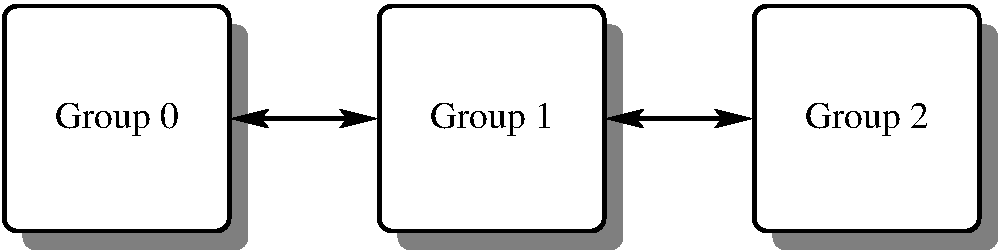
\includegraphics[width=4.0in]{figures/context-fig-1}}
  \caption{Three-group pipeline}
  \label{fig:three-group-pipeline}
\end{figure}


%\begin{verbatim}
%
              %+---------+         +---------+         +---------+
              %|         |         |         |         |         |
              %| Group 0 | <-----> | Group 1 | <-----> | Group 2 |
              %|         |         |         |         |         |
              %+---------+         +---------+         +---------+
%
%\end{verbatim}

As shown in Figure~\ref{fig:three-group-pipeline},
groups~0 and~1 communicate. Groups~1 and~2 communicate. Therefore, group~0
requires one inter-communicator, group~1 requires two
inter-communicators, and group~2 requires 1 inter-communicator.


\begin{example}
\Exindex{C}{Three-Group ``Pipeline''}{MPI\_Comm\_split,MPI\_Intercomm\_create}%
%%HEADER
%%LANG: C
%%SKIPELIPSIS
%%ENDHEADER
\begin{lstlisting}[language={[MPI]C},basicstyle=\lstsmall]
int main(int argc, char *argv[])
{
  MPI_Comm   myComm;       /* intra-communicator of local sub-group */
  MPI_Comm   myFirstComm;  /* inter-communicator */
  MPI_Comm   mySecondComm; /* second inter-communicator (group 1 only) */
  int membershipKey;
  int rank;

  MPI_Init(&argc, &argv);
  MPI_Comm_rank(MPI_COMM_WORLD, &rank);

  /* User code must generate membershipKey in the range [0, 1, 2] */
  membershipKey = rank % 3;

  /* Build intra-communicator for local sub-group */
  MPI_Comm_split(MPI_COMM_WORLD, membershipKey, rank, &myComm);

  /* Build inter-communicators. Tags are hard-coded. */
  if (membershipKey == 0)
  {                     /* Group 0 communicates with group 1. */
    MPI_Intercomm_create(myComm, 0, MPI_COMM_WORLD, 1,
                         1, &myFirstComm);
  }
  else if (membershipKey == 1)
  {              /* Group 1 communicates with groups 0 and 2. */
    MPI_Intercomm_create(myComm, 0, MPI_COMM_WORLD, 0,
                         1, &myFirstComm);
    MPI_Intercomm_create(myComm, 0, MPI_COMM_WORLD, 2,
                         12, &mySecondComm);
  }
  else if (membershipKey == 2)
  {                     /* Group 2 communicates with group 1. */
    MPI_Intercomm_create(myComm, 0, MPI_COMM_WORLD, 1,
                         12, &myFirstComm);
  }

  /* Do work ... */

  switch(membershipKey)  /* free communicators appropriately */
  {
  case 1:
     MPI_Comm_free(&mySecondComm);
  case 0:
  case 2:
     MPI_Comm_free(&myFirstComm);
     break;
  }

  MPI_Finalize();
  return 0;
}
\end{lstlisting}
\end{example}

\subsubsection{Example 2:  Three-Group ``Ring''}
\label{context-ex8}

\begin{figure}
  \centerline{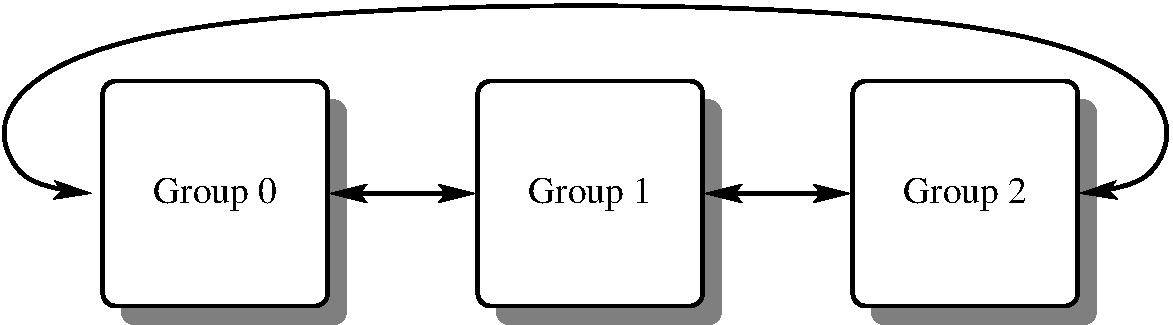
\includegraphics[width=4.0in]{figures/context-fig-2}}
  \caption{Three-group ring}
  \label{fig:three-group-ring}
\end{figure}

%\begin{verbatim}
         %+-----------------------------------------------------------+
         %|                                                           |
         %|    +---------+         +---------+         +---------+    |
         %|    |         |         |         |         |         |    |
         %+--> | Group 0 | <-----> | Group 1 | <-----> | Group 2 | <--+
 %             |         |         |         |         |         |
              %+---------+         +---------+         +---------+
%\end{verbatim}

As shown in Figure~\ref{fig:three-group-ring},
groups~0 and~1 communicate. Groups~1 and~2 communicate. Groups~0 and~2
communicate. Therefore, each requires two inter-communicators.

\begin{example}
\Exindex{C}{Three-Group ``Ring''}{MPI\_Comm\_split,MPI\_Intercomm\_create}%
%%HEADER
%%LANG: C
%%SKIPELIPSIS
%%ENDHEADER
\begin{lstlisting}[language={[MPI]C}]
int main(int argc, char *argv[])
{
  MPI_Comm   myComm;      /* intra-communicator of local sub-group */
  MPI_Comm   myFirstComm; /* inter-communicators */
  MPI_Comm   mySecondComm;
  int membershipKey;
  int rank;

  MPI_Init(&argc, &argv);
  MPI_Comm_rank(MPI_COMM_WORLD, &rank);
  ...

  /* User code must generate membershipKey in the range [0, 1, 2] */
  membershipKey = rank % 3;

  /* Build intra-communicator for local sub-group */
  MPI_Comm_split(MPI_COMM_WORLD, membershipKey, rank, &myComm);

  /* Build inter-communicators. Tags are hard-coded. */
  if (membershipKey == 0)
  {             /* Group 0 communicates with groups 1 and 2. */
    MPI_Intercomm_create(myComm, 0, MPI_COMM_WORLD, 1,
                         1, &myFirstComm);
    MPI_Intercomm_create(myComm, 0, MPI_COMM_WORLD, 2,
                         2, &mySecondComm);
  }
  else if (membershipKey == 1)
  {         /* Group 1 communicates with groups 0 and 2. */
    MPI_Intercomm_create(myComm, 0, MPI_COMM_WORLD, 0,
                         1, &myFirstComm);
    MPI_Intercomm_create(myComm, 0, MPI_COMM_WORLD, 2,
                         12, &mySecondComm);
  }
  else if (membershipKey == 2)
  {        /* Group 2 communicates with groups 0 and 1. */
    MPI_Intercomm_create(myComm, 0, MPI_COMM_WORLD, 0,
                         2, &myFirstComm);
    MPI_Intercomm_create(myComm, 0, MPI_COMM_WORLD, 1,
                         12, &mySecondComm);
  }

  /* Do some work ... */

  /* Then free communicators before terminating... */
  MPI_Comm_free(&myFirstComm);
  MPI_Comm_free(&mySecondComm);
  MPI_Comm_free(&myComm);
  MPI_Finalize();
  return 0;
}
\end{lstlisting}
\end{example}
  
\section{Caching} 
\mpitermtitleindex{caching}
\label{sec:caching}

\MPI/ provides a ``caching'' facility that allows an application to
attach arbitrary pieces of information, called \mpitermdefni{attributes}\mpitermdefindex{attribute}, to
three kinds of \MPI/ objects: communicators,
windows, and datatypes.
More precisely, the caching
facility allows a portable library to do the following:
\begin{itemize}
\item
  pass information between calls by associating it
  with an \MPI/ intra- or inter\hyphen/communicator,
window, or datatype,
\item quickly retrieve that information, and
\item
 be guaranteed that out-of-date information is never retrieved, even if
 the object is freed and its handle subsequently reused by \MPI/.
\end{itemize}

The caching capabilities, in some form, are required by built-in \MPI/ routines
such as collective communication and application topology. Defining an
interface to these capabilities as part of the \MPI/ standard is valuable
because it permits routines like collective communication and application
topologies to be implemented as portable code, and also because it makes \MPI/
more extensible by allowing user-written routines to use standard \MPI/ calling
sequences.

\begin{users}
The communicator \mpiconst{MPI\_COMM\_SELF} is a suitable choice for posting
\MPI/ process-local attributes, via this
attribute-caching mechanism.
\end{users}


\begin{rationale}
In one extreme 
one
can allow caching on all opaque handles. The other
extreme is to only allow it on communicators. Caching has a cost
associated with it and should only be allowed when it is clearly needed and
the increased cost is modest.
This is the reason that windows and datatypes were
added but not other handles.
\end{rationale}

One difficulty
is the potential for size differences between
Fortran integers and C pointers.
For this reason, the
Fortran versions of these routines
use integers of kind \mpiconst{MPI\_ADDRESS\_KIND}.
\begin{implementors}
High-quality implementations should raise an error when a keyval
\mpifuncindex{MPI\_TYPE\_CREATE\_KEYVAL}%
\mpifuncindex{MPI\_COMM\_CREATE\_KEYVAL}%
\mpifuncindex{MPI\_WIN\_CREATE\_KEYVAL}%
that was created by a call to \mpiskipfunc{MPI\_\XXX/\_CREATE\_KEYVAL} is
used with an object of the wrong type with a call to
\mpifuncindex{MPI\_COMM\_GET\_ATTR}\mpifuncindex{MPI\_COMM\_SET\_ATTR}\mpifuncindex{MPI\_COMM\_DELETE\_ATTR}\mpifuncindex{MPI\_COMM\_FREE\_KEYVAL}%
\mpifuncindex{MPI\_TYPE\_GET\_ATTR}\mpifuncindex{MPI\_TYPE\_SET\_ATTR}\mpifuncindex{MPI\_TYPE\_DELETE\_ATTR}\mpifuncindex{MPI\_TYPE\_FREE\_KEYVAL}%
\mpifuncindex{MPI\_WIN\_GET\_ATTR}\mpifuncindex{MPI\_WIN\_SET\_ATTR}\mpifuncindex{MPI\_WIN\_DELETE\_ATTR}\mpifuncindex{MPI\_WIN\_FREE\_KEYVAL}%
\mpiskipfunc{MPI\_YYY\_GET\_ATTR}, \mpiskipfunc{MPI\_YYY\_SET\_ATTR}, \mpiskipfunc{MPI\_YYY\_DELETE\_ATTR}, or
\mpiskipfunc{MPI\_YYY\_FREE\_KEYVAL}. To do so, it is necessary to maintain, with
each keyval, information on the type of the associated user
function.
\end{implementors}

\subsection{Functionality}
\label{subsec:context-cachefunc}

Attributes
can be
attached to communicators,
windows, and datatypes.
Attributes are local to the \MPI/ process and specific to the communicator
to which they are attached. Attributes are not propagated by \MPI/ from one
communicator to another except when the communicator is duplicated
using \mpifunc{MPI\_COMM\_DUP}, \mpifunc{MPI\_COMM\_IDUP},
\mpifunc{MPI\_COMM\_DUP\_WITH\_INFO}, and \mpifunc{MPI\_COMM\_IDUP\_WITH\_INFO}
(and even then the application must give specific permission through
callback functions for the attribute to be copied. Please refer to
Section~\ref{subsec:context-intracomconst} and Section~\ref{subsec:context-cachecomm}
for attributes propagation rules).

\begin{users}
Attributes in C are of type \code{void*}. Typically, such an attribute
will be a pointer to a structure that contains further information, or
a handle to an \MPI/ object.
In Fortran, attributes are of type \ftype{INTEGER}. Such attribute
can be a handle to an \MPI/ object, or just an integer-valued
attribute.
\end{users}

\begin{implementors}
Attributes are scalar values, equal in size to, or larger than a C-language
pointer. Attributes can always hold an \MPI/ handle.
\end{implementors}

The caching interface defined here
requires
that attributes be
stored by \MPI/ opaquely within a communicator,
window, or datatype.
Accessor functions include the following:
\begin{itemize}
\item
 obtain a key value (used to identify an attribute); the user
 specifies ``callback'' functions by which \MPI/ informs the application
 when the communicator is destroyed or
 copied.
\item
 store and retrieve the value of an attribute;
\end{itemize}

\begin{implementors}
Caching and callback functions are only called synchronously,
in response to explicit application requests. This avoids problems
that result from repeated crossings between user and system space.
(This synchronous calling rule is a general property of \MPI/.)

The choice of key values is under control of \MPI/. This allows \MPI/ to optimize
its implementation of attribute sets. It also avoids conflict between
independent modules caching information on the same communicators.

A much smaller interface, consisting of just a callback facility, would allow
the entire caching facility to be implemented by portable code. However, with
the minimal callback interface, some form of table searching is implied by the
need to handle arbitrary communicators. In contrast, the more complete
interface defined here permits rapid access to attributes through the use of
pointers in communicators (to find the attribute table) and cleverly chosen
key values (to retrieve individual attributes). In light of the efficiency
``hit'' inherent in the minimal interface, the more complete interface defined
here is seen to be superior.
\end{implementors}

\noindent \MPI/ provides the following services related to caching. They are
all \MPI/ process local.

%%%%%%%%%%%%%%%%%%%%%%%%%%%%%%%%%%%%%%%%%%%%%%%%%%%%%%%%%%%%%%%%%%%%%%
\subsection{Communicators}
\label{subsec:context-cachecomm}

% The new functions that are replacements for the \mpii/ functions 
Functions
for caching on communicators are:

\begin{funcdef}{MPI\_COMM\_CREATE\_KEYVAL}{(\mbox{comm\_copy\_attr\_fn}, \mbox{comm\_delete\_attr\_fn}, \mbox{comm\_keyval}, \mbox{extra\_state})}
\funcarg{\IN}{comm\_copy\_attr\_fn}{copy callback function for \mpiarg{comm\_keyval} (function)}
\funcarg{\IN}{comm\_delete\_attr\_fn}{delete callback function for \mpiarg{comm\_keyval} (function)}
\funcarg{\OUT}{comm\_keyval}{key value for future access (integer)}
\funcarg{\IN}{extra\_state}{extra state for callback function}
\end{funcdef}
\mpicallbackindex{MPI\_Comm\_copy\_attr\_function}%
\mpicallbackindex{MPI\_Comm\_delete\_attr\_function}%
\mpibindmain{MPI\_Comm\_create\_keyval}{(\gb{}MPI\_Comm\_copy\_attr\_function~*comm\_copy\_attr\_fn, MPI\_Comm\_delete\_attr\_function~*comm\_delete\_attr\_fn, int~*comm\_keyval, void~*extra\_state)}
\mpifnewbindmain{MPI\_Comm\_create\_keyval}{(comm\_copy\_attr\_fn, comm\_delete\_attr\_fn, comm\_keyval, extra\_state, ierror) \fargs PROCEDURE(MPI\_Comm\_copy\_attr\_function)\ ::\ \mbox{comm\_copy\_attr\_fn}\fnarg{}PROCEDURE(MPI\_Comm\_delete\_attr\_function)\ ::\ \mbox{comm\_delete\_attr\_fn}\fnarg{}INTEGER, INTENT(OUT)\ ::\ \mbox{comm\_keyval}\fnarg{}INTEGER(KIND=MPI\_ADDRESS\_KIND), INTENT(IN)\ ::\ \mbox{extra\_state}\fnfinalarg{}INTEGER, OPTIONAL, INTENT(OUT)\ ::\ \mbox{ierror}}
\mpicallbackindex{COMM\_COPY\_ATTR\_FUNCTION}%
\mpicallbackindex{COMM\_DELETE\_ATTR\_FUNCTION}%
\mpifbindmain{MPI\_COMM\_CREATE\_KEYVAL}{(COMM\_COPY\_ATTR\_FN, COMM\_DELETE\_ATTR\_FN, COMM\_KEYVAL, EXTRA\_STATE, IERROR) \fargs EXTERNAL \mbox{COMM\_COPY\_ATTR\_FN}, \mbox{COMM\_DELETE\_ATTR\_FN}\fnarg{}INTEGER \mbox{COMM\_KEYVAL}, \mbox{IERROR}\fnfinalarg{}INTEGER(KIND=MPI\_ADDRESS\_KIND) \mbox{EXTRA\_STATE}}

Generates a new attribute key. Keys are locally unique in an \MPI/ process,
and opaque to user, though they are explicitly stored in integers.
Once allocated, the key value can be used to associate attributes
and access them on any locally defined communicator.

\noindent
The C callback functions are:

\cdeclindex{MPI\_Comm}%
\mpitypedefbindmain{MPI\_Comm\_copy\_attr\_function}{(\gb{}MPI\_Comm~oldcomm, int~comm\_keyval, void~*extra\_state, void~*attribute\_val\_in, void~*attribute\_val\_out, int~*flag)}


\noindent
and

\cdeclindex{MPI\_Comm}%
\mpitypedefbindmain{MPI\_Comm\_delete\_attr\_function}{(\gb{}MPI\_Comm~comm, int~comm\_keyval, void~*attribute\_val, void~*extra\_state)}

\noindent
which are the same as the \mpiidoti/ calls but with a new name.
The old names are deprecated.

\noindent
With the \code{mpi\_f08} module, the Fortran callback functions are:

\mpifnewsubbind{MPI\_Comm\_copy\_attr\_function}{(oldcomm, comm\_keyval, extra\_state, attribute\_val\_in, attribute\_val\_out, flag, ierror) \fargs TYPE(MPI\_Comm)\ ::\ \mbox{oldcomm}\fnarg{}INTEGER\ ::\ \mbox{comm\_keyval}, \mbox{ierror}\fnarg{}INTEGER(KIND=MPI\_ADDRESS\_KIND)\ ::\ \mbox{extra\_state}, \mbox{attribute\_val\_in}, \mbox{attribute\_val\_out}\fnfinalarg{}LOGICAL\ ::\ \mbox{flag}}
 
\noindent
and
 
\mpifnewsubbind{MPI\_Comm\_delete\_attr\_function}{(comm, comm\_keyval, attribute\_val, extra\_state, ierror) \fargs TYPE(MPI\_Comm)\ ::\ \mbox{comm}\fnarg{}INTEGER\ ::\ \mbox{comm\_keyval}, \mbox{ierror}\fnfinalarg{}INTEGER(KIND=MPI\_ADDRESS\_KIND)\ ::\ \mbox{attribute\_val}, \mbox{extra\_state}}

\noindent
With the \code{mpi} module and (deprecated) \code{mpif.h} include file, the Fortran callback functions are:

\mpifsubbindmain{COMM\_COPY\_ATTR\_FUNCTION}{(OLDCOMM, COMM\_KEYVAL, EXTRA\_STATE, ATTRIBUTE\_VAL\_IN, ATTRIBUTE\_VAL\_OUT, FLAG, IERROR) \fargs INTEGER \mbox{OLDCOMM}, \mbox{COMM\_KEYVAL}, \mbox{IERROR}\fnarg{}INTEGER(KIND=MPI\_ADDRESS\_KIND) \mbox{EXTRA\_STATE}, \mbox{ATTRIBUTE\_VAL\_IN}, \mbox{ATTRIBUTE\_VAL\_OUT}\fnfinalarg{}LOGICAL \mbox{FLAG}}

\noindent
and

\mpifsubbindmain{COMM\_DELETE\_ATTR\_FUNCTION}{(COMM, COMM\_KEYVAL, ATTRIBUTE\_VAL, EXTRA\_STATE, IERROR) \fargs INTEGER \mbox{COMM}, \mbox{COMM\_KEYVAL}, \mbox{IERROR}\fnfinalarg{}INTEGER(KIND=MPI\_ADDRESS\_KIND) \mbox{ATTRIBUTE\_VAL}, \mbox{EXTRA\_STATE}}

The \mpiarg{comm\_copy\_attr\_fn} function is invoked when a communicator is
duplicated by \mpifunc{MPI\_COMM\_DUP}, \mpifunc{MPI\_COMM\_IDUP}, \mpifunc{MPI\_COMM\_DUP\_WITH\_INFO}
or \mpifunc{MPI\_COMM\_IDUP\_WITH\_INFO}.
\mpiarg{comm\_copy\_attr\_fn} should be
of type \mpicallbackskip{MPI\_Comm\_copy\_attr\_function}.
The copy callback function is invoked for each key value in
\mpiarg{oldcomm} in arbitrary order. Each call
to the copy callback is made with a key value and its corresponding attribute.
If it returns \mpiarg{flag}\mpicode{ = 0} or \code{.FALSE.}, then the
attribute is deleted in the duplicated communicator. Otherwise
(\mpiarg{flag}\mpicode{ = 1} or \code{.TRUE.}),
the new attribute value is set to the value
returned in
\mpiarg{attribute\_val\_out}.
The function returns \error{MPI\_SUCCESS} on
success and an error code on failure (in which case
\mpifunc{MPI\_COMM\_DUP} or \mpifunc{MPI\_COMM\_IDUP} will fail).

The argument \mpiarg{comm\_copy\_attr\_fn} may be specified as
\mpiconstfuncmain{MPI\_COMM\_NULL\_COPY\_FN} or
\mpiconstfuncmain{MPI\_COMM\_DUP\_FN}
from either C or Fortran.
\mpiconstfunc{MPI\_COMM\_NULL\_COPY\_FN}
is a function that does nothing other than returning \mpiarg{flag}\mpicode{ = 0}
or \code{.FALSE.} (depending on whether the keyval
 was created with a C or Fortran binding to
 \mpifunc{MPI\_COMM\_CREATE\_KEYVAL}) and \error{MPI\_SUCCESS}.
\mpiconstfunc{MPI\_COMM\_DUP\_FN} is a simple
copy function that sets \mpiarg{flag}\mpicode{ = 1} or \code{.TRUE.},
returns the value of
\mpiarg{attribute\_val\_in} in \mpiarg{attribute\_val\_out}, and
returns \error{MPI\_SUCCESS}.
These replace the \mpii/ predefined callbacks \mpiconstfunc{MPI\_NULL\_COPY\_FN}
and \mpiconstfunc{MPI\_DUP\_FN}, whose use is deprecated.

% The following declarations are needed for generating the
% list of functions in the annex.
% They are not used for printing here.
% Therefore, they are surrounded by a deleting macro.
\OnlyForAutomaticAnnexGeneration{%
\mpibindmain{MPI\_COMM\_NULL\_COPY\_FN}{(\gb{}MPI\_Comm~oldcomm, int~comm\_keyval, void~*extra\_state, void~*attribute\_val\_in, void~*attribute\_val\_out, int~*flag)}
\mpifnewbindmain{MPI\_COMM\_NULL\_COPY\_FN}{(oldcomm, comm\_keyval, extra\_state, attribute\_val\_in, attribute\_val\_out, flag, ierror) \fargs TYPE(MPI\_Comm)\ ::\ \mbox{oldcomm}\fnarg{}INTEGER\ ::\ \mbox{comm\_keyval}, \mbox{ierror}\fnarg{}INTEGER(KIND=MPI\_ADDRESS\_KIND)\ ::\ \mbox{extra\_state}, \mbox{attribute\_val\_in}, \mbox{attribute\_val\_out}\fnfinalarg{}LOGICAL\ ::\ \mbox{flag}}
\mpifbindmain{MPI\_COMM\_NULL\_COPY\_FN}{(OLDCOMM, COMM\_KEYVAL, EXTRA\_STATE, ATTRIBUTE\_VAL\_IN, ATTRIBUTE\_VAL\_OUT, FLAG, IERROR) \fargs INTEGER \mbox{OLDCOMM}, \mbox{COMM\_KEYVAL}, \mbox{IERROR}\fnarg{}INTEGER(KIND=MPI\_ADDRESS\_KIND) \mbox{EXTRA\_STATE}, \mbox{ATTRIBUTE\_VAL\_IN}, \mbox{ATTRIBUTE\_VAL\_OUT}\fnfinalarg{}LOGICAL \mbox{FLAG}}
}%

\OnlyForAutomaticAnnexGeneration{%
\mpibindmain{MPI\_COMM\_DUP\_FN}{(\gb{}MPI\_Comm~oldcomm, int~comm\_keyval, void~*extra\_state, void~*attribute\_val\_in, void~*attribute\_val\_out, int~*flag)}
\mpifnewbindmain{MPI\_COMM\_DUP\_FN}{(oldcomm, comm\_keyval, extra\_state, attribute\_val\_in, attribute\_val\_out, flag, ierror) \fargs TYPE(MPI\_Comm)\ ::\ \mbox{oldcomm}\fnarg{}INTEGER\ ::\ \mbox{comm\_keyval}, \mbox{ierror}\fnarg{}INTEGER(KIND=MPI\_ADDRESS\_KIND)\ ::\ \mbox{extra\_state}, \mbox{attribute\_val\_in}, \mbox{attribute\_val\_out}\fnfinalarg{}LOGICAL\ ::\ \mbox{flag}}
\mpifbindmain{MPI\_COMM\_DUP\_FN}{(OLDCOMM, COMM\_KEYVAL, EXTRA\_STATE, ATTRIBUTE\_VAL\_IN, ATTRIBUTE\_VAL\_OUT, FLAG, IERROR) \fargs INTEGER \mbox{OLDCOMM}, \mbox{COMM\_KEYVAL}, \mbox{IERROR}\fnarg{}INTEGER(KIND=MPI\_ADDRESS\_KIND) \mbox{EXTRA\_STATE}, \mbox{ATTRIBUTE\_VAL\_IN}, \mbox{ATTRIBUTE\_VAL\_OUT}\fnfinalarg{}LOGICAL \mbox{FLAG}}
}%

\begin{users}
Even though both formal arguments \mpiarg{attribute\_val\_in} and
\mpiarg{attribute\_val\_out} are of type \code{void*}, their usage differs.
The C copy function is passed by \MPI/ in \mpiarg{attribute\_val\_in}
the \emph{value} of the attribute, and in
\mpiarg{attribute\_val\_out} the \emph{address} of the attribute, so as
to allow the function to return the (new) attribute value.
The use of type \code{void*} for both is to avoid messy type casts.

A valid copy function is one that completely duplicates the
information by making a full duplicate copy of the data structures
implied by an attribute; another might just make another reference to
that data structure, while using a reference-count mechanism. Other
types of attributes might not copy at all (they might be specific to
\mpiarg{oldcomm} only).
\end{users}

\begin{implementors}
A C interface should be assumed for copy and delete functions
associated with key values created in C; a Fortran calling interface
should be assumed for key values created in Fortran.
\end{implementors}

Analogous to \mpiarg{comm\_copy\_attr\_fn} is a callback deletion function, defined
as follows. The \mpiarg{comm\_delete\_attr\_fn} function is invoked when a communicator is
deleted by \mpifunc{MPI\_COMM\_FREE}, \mpifunc{MPI\_COMM\_DISCONNECT} or when a call is made explicitly to
\mpifunc{MPI\_COMM\_DELETE\_ATTR}.
\mpiarg{comm\_delete\_attr\_fn} should be
of type \mpicallbackskip{MPI\_Comm\_delete\_attr\_function}.

This function is called by \mpifunc{MPI\_COMM\_FREE},
\mpifunc{MPI\_COMM\_DISCONNECT},
\mpifunc{MPI\_COMM\_DELETE\_ATTR},
and \mpifunc{MPI\_COMM\_SET\_ATTR}
to do whatever is needed to remove an attribute.
The function returns \error{MPI\_SUCCESS} on
success and an error code on failure (in which case
\mpifunc{MPI\_COMM\_FREE} will fail).

% RAB: The predefined callbacks are "constant" "function" pointers, therefore in both indexes
The argument \mpiarg{comm\_delete\_attr\_fn} may be specified as\flushline % fix for margin
\mpiconstfuncmain{MPI\_COMM\_NULL\_DELETE\_FN}
from either C or Fortran.\flushline % fix for margin
\mpiconstfuncskip{MPI\_COMM\_NULL\_DELETE\_FN} is a function that does nothing, other
than returning \error{MPI\_SUCCESS}. \mpiconstfunc{MPI\_COMM\_NULL\_DELETE\_FN}
replaces \mpiconstfunc{MPI\_NULL\_DELETE\_FN}, whose use is deprecated.

% The following declarations are needed for generating the
% list of functions in the annex.
% They are not used for printing here.
% Therefore, they are surrounded by a deleting macro.
\OnlyForAutomaticAnnexGeneration{%
\mpibindmain{MPI\_COMM\_NULL\_DELETE\_FN}{(\gb{}MPI\_Comm~comm, int~comm\_keyval, void~*attribute\_val, void~*extra\_state)}
\mpifnewbindmain{MPI\_COMM\_NULL\_DELETE\_FN}{(comm, comm\_keyval, attribute\_val, extra\_state, ierror) \fargs TYPE(MPI\_Comm)\ ::\ \mbox{comm}\fnarg{}INTEGER\ ::\ \mbox{comm\_keyval}, \mbox{ierror}\fnfinalarg{}INTEGER(KIND=MPI\_ADDRESS\_KIND)\ ::\ \mbox{attribute\_val}, \mbox{extra\_state}}
\mpifbindmain{MPI\_COMM\_NULL\_DELETE\_FN}{(COMM, COMM\_KEYVAL, ATTRIBUTE\_VAL, EXTRA\_STATE, IERROR) \fargs INTEGER \mbox{COMM}, \mbox{COMM\_KEYVAL}, \mbox{IERROR}\fnfinalarg{}INTEGER(KIND=MPI\_ADDRESS\_KIND) \mbox{ATTRIBUTE\_VAL}, \mbox{EXTRA\_STATE}}
}%

If an attribute copy function or attribute delete function returns other than
\error{MPI\_SUCCESS}, then the call that caused it to be invoked (for example,
\mpifunc{MPI\_COMM\_FREE}) is erroneous.


The special key value \mpiconstmain{MPI\_KEYVAL\_INVALID} is never returned
by \mpifunc{MPI\_COMM\_CREATE\_KEYVAL}. Therefore, it can be used for
static initialization of key values.

\begin{implementors}
\label{advice:context:predefined:Fortran:implementors}%
The predefined Fortran functions \mpiconstfunc{MPI\_COMM\_NULL\_COPY\_FN},
\mpiconstfunc{MPI\_COMM\_DUP\_FN},
and \vlgb\mpiconstfunc{MPI\_COMM\_NULL\_DELETE\_FN} are defined
in the \code{mpi} module (and deprecated \gb\code{mpif.h}) and the \code{mpi\_f08} module
with the same name, but with different interfaces.
Each function can coexist twice with the same name in the same \MPI/ library,
one routine as an implicit interface outside of the \code{mpi} module,
i.e., declared as \ftype{EXTERNAL},
and the other routine within \code{mpi\_f08} declared with \ftype{CONTAINS}.
These routines have different link names, which are also different
to the link names used for the routines used in C.
\end{implementors}

\begin{users}
\label{advice:context:predefined:Fortran:users}%
Callbacks, including the predefined Fortran functions
\mpiconstfunc{MPI\_COMM\_NULL\_COPY\_FN}, \mpiconstfunc{MPI\_COMM\_DUP\_FN},
and \vlgb\mpiconstfunc{MPI\_COMM\_NULL\_DELETE\_FN} should not be passed from one application
routine that uses the \code{mpi\_f08} module to another
application routine that uses the \code{mpi} module or (deprecated) \code{mpif.h} include file,
and vice versa;
see also the advice to users on page~\pageref{advice:bindings:predefined:Fortran:users}.
\end{users}

\begin{funcdef}{MPI\_COMM\_FREE\_KEYVAL}{(\mbox{comm\_keyval})}
\funcarg{\INOUT}{comm\_keyval}{key value (integer)}
\end{funcdef}
\mpibindmain{MPI\_Comm\_free\_keyval}{(\gb{}int~*comm\_keyval)}
\mpifnewbindmain{MPI\_Comm\_free\_keyval}{(comm\_keyval, ierror) \fargs INTEGER, INTENT(INOUT)\ ::\ \mbox{comm\_keyval}\fnfinalarg{}INTEGER, OPTIONAL, INTENT(OUT)\ ::\ \mbox{ierror}}
\mpifbindmain{MPI\_COMM\_FREE\_KEYVAL}{(COMM\_KEYVAL, IERROR) \fargs \fnfinalarg{}INTEGER \mbox{COMM\_KEYVAL}, \mbox{IERROR}}

Frees an extant attribute key.
This function sets the value of \mpiarg{keyval} to
\mpiconst{MPI\_KEYVAL\_INVALID}.
Note that it is not erroneous to free an attribute key
that is in use, because the actual free does not transpire until after all
references (in other communicators on the \MPI/ process) to the key have been freed.
These references need to be explictly freed by the program, either via calls
to \mpifunc{MPI\_COMM\_DELETE\_ATTR} that free one attribute instance, or by calls
to \mpifunc{MPI\_COMM\_FREE} that free all attribute instances associated with
the freed communicator.

\cdeclindex{MPI\_Comm}%
\begin{funcdef}{MPI\_COMM\_SET\_ATTR}{(\mbox{comm}, \mbox{comm\_keyval}, \mbox{attribute\_val})}
\funcarg{\INOUT}{comm}{communicator to which attribute will be attached (handle)}
\funcarg{\IN}{comm\_keyval}{key value (integer)}
\funcarg{\IN}{attribute\_val}{attribute value}
\end{funcdef}
\mpibindmain{MPI\_Comm\_set\_attr}{(\gb{}MPI\_Comm~comm, int~comm\_keyval, void~*attribute\_val)}
\mpifnewbindmain{MPI\_Comm\_set\_attr}{(comm, comm\_keyval, attribute\_val, ierror) \fargs TYPE(MPI\_Comm), INTENT(IN)\ ::\ \mbox{comm}\fnarg{}INTEGER, INTENT(IN)\ ::\ \mbox{comm\_keyval}\fnarg{}INTEGER(KIND=MPI\_ADDRESS\_KIND), INTENT(IN)\ ::\ \mbox{attribute\_val}\fnfinalarg{}INTEGER, OPTIONAL, INTENT(OUT)\ ::\ \mbox{ierror}}
\mpifbindmain{MPI\_COMM\_SET\_ATTR}{(COMM, COMM\_KEYVAL, ATTRIBUTE\_VAL, IERROR) \fargs INTEGER \mbox{COMM}, \mbox{COMM\_KEYVAL}, \mbox{IERROR}\fnfinalarg{}INTEGER(KIND=MPI\_ADDRESS\_KIND) \mbox{ATTRIBUTE\_VAL}}

This function stores the stipulated attribute value \mpiarg{attribute\_val}
for subsequent retrieval by \mpifunc{MPI\_COMM\_GET\_ATTR}.
If the value is already present, then the outcome
is as if \mpifunc{MPI\_COMM\_DELETE\_ATTR} %mansplit
was first called to delete the previous
value (and the callback function \mpiarg{comm\_delete\_attr\_fn} was executed), and a new
value was next stored. The call is erroneous if there is no key with value
\mpiarg{keyval}; in particular
\mpiconst{MPI\_KEYVAL\_INVALID} is an erroneous key value.
The call will fail if the \mpiarg{comm\_delete\_attr\_fn} function returned an error code
other than \error{MPI\_SUCCESS}.

\cdeclindex{MPI\_Comm}%
\begin{funcdef}{MPI\_COMM\_GET\_ATTR}{(\mbox{comm}, \mbox{comm\_keyval}, \mbox{attribute\_val}, \mbox{flag})}
\funcarg{\IN}{comm}{communicator to which the attribute is attached (handle)}
\funcarg{\IN}{comm\_keyval}{key value (integer)}
\funcarg{\OUT}{attribute\_val}{attribute value, unless \mpiarg{flag}\mpicode{ = false}}
\funcarg{\OUT}{flag}{\mpicode{false} if no attribute is associated with the key (logical)}
\end{funcdef}
\mpibindmain{MPI\_Comm\_get\_attr}{(\gb{}MPI\_Comm~comm, int~comm\_keyval, void~*attribute\_val, int~*flag)}
\mpifnewbindmain{MPI\_Comm\_get\_attr}{(comm, comm\_keyval, attribute\_val, flag, ierror) \fargs TYPE(MPI\_Comm), INTENT(IN)\ ::\ \mbox{comm}\fnarg{}INTEGER, INTENT(IN)\ ::\ \mbox{comm\_keyval}\fnarg{}INTEGER(KIND=MPI\_ADDRESS\_KIND), INTENT(OUT)\ ::\ \mbox{attribute\_val}\fnarg{}LOGICAL, INTENT(OUT)\ ::\ \mbox{flag}\fnfinalarg{}INTEGER, OPTIONAL, INTENT(OUT)\ ::\ \mbox{ierror}}
\mpifbindmain{MPI\_COMM\_GET\_ATTR}{(COMM, COMM\_KEYVAL, ATTRIBUTE\_VAL, FLAG, IERROR) \fargs INTEGER \mbox{COMM}, \mbox{COMM\_KEYVAL}, \mbox{IERROR}\fnarg{}INTEGER(KIND=MPI\_ADDRESS\_KIND) \mbox{ATTRIBUTE\_VAL}\fnfinalarg{}LOGICAL \mbox{FLAG}}

Retrieves attribute value by key.
The call is erroneous if there is no key with value
\mpiarg{keyval}. On the other hand, the call is correct if the key value
exists, but no attribute is attached on \mpiarg{comm} for that key; in such case,
the call returns \mpicode{flag}\mpicode{ = false}. In particular
\mpiconst{MPI\_KEYVAL\_INVALID} is an erroneous key value.

\begin{users}
The call to \cfunc{MPI\_Comm\_set\_attr} passes in \mpiarg{attribute\_val}
the \emph{value} of the attribute; the call to \cfunc{MPI\_Comm\_get\_attr}
passes in \mpiarg{attribute\_val} the \emph{address} of
the
location where the attribute value is to be returned.
Thus, if the attribute value itself is a pointer of type \code{void*}, 
then the
actual \mpiarg{attribute\_val} parameter to
\cfunc{MPI\_Comm\_set\_attr} will be of type \code{void*} and the actual
\mpiarg{attribute\_val} parameter to
\cfunc{MPI\_Comm\_get\_attr}
will be of type \code{void**}.
\end{users}

\begin{rationale}
The use of a formal parameter \mpiarg{attribute\_val}
of type
\code{void*} (rather than \code{void**}) avoids the messy type
casting that would be needed if the attribute value is declared with a
type other than \code{void*}.
\end{rationale}

\cdeclindex{MPI\_Comm}%
\begin{funcdef}{MPI\_COMM\_DELETE\_ATTR}{(\mbox{comm}, \mbox{comm\_keyval})}
\funcarg{\INOUT}{comm}{communicator from which the attribute is deleted (handle)}
\funcarg{\IN}{comm\_keyval}{key value (integer)}
\end{funcdef}
\mpibindmain{MPI\_Comm\_delete\_attr}{(\gb{}MPI\_Comm~comm, int~comm\_keyval)}
\mpifnewbindmain{MPI\_Comm\_delete\_attr}{(comm, comm\_keyval, ierror) \fargs TYPE(MPI\_Comm), INTENT(IN)\ ::\ \mbox{comm}\fnarg{}INTEGER, INTENT(IN)\ ::\ \mbox{comm\_keyval}\fnfinalarg{}INTEGER, OPTIONAL, INTENT(OUT)\ ::\ \mbox{ierror}}
\mpifbindmain{MPI\_COMM\_DELETE\_ATTR}{(COMM, COMM\_KEYVAL, IERROR) \fargs \fnfinalarg{}INTEGER \mbox{COMM}, \mbox{COMM\_KEYVAL}, \mbox{IERROR}}

Delete attribute from cache by key. This function invokes the
attribute delete function \mpiarg{comm\_delete\_attr\_fn}
specified when the \mpiarg{keyval} was created.
The call will fail if the \mpiarg{comm\_delete\_attr\_fn} function returns an
error code other than \error{MPI\_SUCCESS}.

Whenever a communicator is replicated using the function
\mpifunc{MPI\_COMM\_DUP}, \mpifunc{MPI\_COMM\_IDUP},
\mpifunc{MPI\_COMM\_DUP\_WITH\_INFO} or \mpifunc{MPI\_COMM\_IDUP\_WITH\_INFO},
all call-back copy functions for attributes
that are currently set are invoked (in arbitrary order).
Whenever a communicator is deleted using the function
\mpifunc{MPI\_COMM\_FREE} all callback delete functions for attributes
that are currently set are invoked.

%%%%%%%%%%%%%%%%%%%%%%%%%%%%%%%%%%%%%%%%%%%%%%%%%%%%%%%%%%%%%%%%%%%%%%
\subsection{Windows}
\label{sec:ei-attr:windows}

The functions for caching on windows are:

\begin{funcdef}{MPI\_WIN\_CREATE\_KEYVAL}{(\mbox{win\_copy\_attr\_fn}, \mbox{win\_delete\_attr\_fn}, \mbox{win\_keyval}, \mbox{extra\_state})}
\funcarg{\IN}{win\_copy\_attr\_fn}{copy callback function for \mpiarg{win\_keyval} (function)}
\funcarg{\IN}{win\_delete\_attr\_fn}{delete callback function for \mpiarg{win\_keyval} (function)}
\funcarg{\OUT}{win\_keyval}{key value for future access (integer)}
\funcarg{\IN}{extra\_state}{extra state for callback function}
\end{funcdef}
\mpicallbackindex{MPI\_Win\_copy\_attr\_function}%
\mpicallbackindex{MPI\_Win\_delete\_attr\_function}%
\mpibindmain{MPI\_Win\_create\_keyval}{(\gb{}MPI\_Win\_copy\_attr\_function~*win\_copy\_attr\_fn, MPI\_Win\_delete\_attr\_function~*win\_delete\_attr\_fn, int~*win\_keyval, void~*extra\_state)}
\mpifnewbindmain{MPI\_Win\_create\_keyval}{(win\_copy\_attr\_fn, win\_delete\_attr\_fn, win\_keyval, extra\_state, ierror) \fargs PROCEDURE(MPI\_Win\_copy\_attr\_function)\ ::\ \mbox{win\_copy\_attr\_fn}\fnarg{}PROCEDURE(MPI\_Win\_delete\_attr\_function)\ ::\ \mbox{win\_delete\_attr\_fn}\fnarg{}INTEGER, INTENT(OUT)\ ::\ \mbox{win\_keyval}\fnarg{}INTEGER(KIND=MPI\_ADDRESS\_KIND), INTENT(IN)\ ::\ \mbox{extra\_state}\fnfinalarg{}INTEGER, OPTIONAL, INTENT(OUT)\ ::\ \mbox{ierror}}
\mpicallbackindex{WIN\_COPY\_ATTR\_FUNCTION}%
\mpicallbackindex{WIN\_DELETE\_ATTR\_FUNCTION}%
\mpifbindmain{MPI\_WIN\_CREATE\_KEYVAL}{(WIN\_COPY\_ATTR\_FN, WIN\_DELETE\_ATTR\_FN, WIN\_KEYVAL, EXTRA\_STATE, IERROR) \fargs EXTERNAL \mbox{WIN\_COPY\_ATTR\_FN}, \mbox{WIN\_DELETE\_ATTR\_FN}\fnarg{}INTEGER \mbox{WIN\_KEYVAL}, \mbox{IERROR}\fnfinalarg{}INTEGER(KIND=MPI\_ADDRESS\_KIND) \mbox{EXTRA\_STATE}}

% RAB: The predefined callbacks are "constant" "function" pointers, therefore in both indexes
The argument \mpiarg{win\_copy\_attr\_fn} may be specified as
\mpiconstfuncmain{MPI\_WIN\_NULL\_COPY\_FN} or
\mpiconstfuncmain{MPI\_WIN\_DUP\_FN}
from either C or Fortran.
\mpiconstfunc{MPI\_WIN\_NULL\_COPY\_FN}
is a function that does nothing other than returning \mpiarg{flag}\mpicode{ = 0}
and \error{MPI\_SUCCESS}.
\mpiconstfunc{MPI\_WIN\_DUP\_FN} is a simple
copy function that sets \mpiarg{flag}\mpicode{ = 1},
returns the value of
\mpiarg{attribute\_val\_in} in \mpiarg{attribute\_val\_out}, and
returns \error{MPI\_SUCCESS}.

% The following declarations are needed for generating the
% list of functions in the annex.
% They are not used for printing here.
% Therefore, they are surrounded by a deleting macro.
\OnlyForAutomaticAnnexGeneration{%
\mpibindmain{MPI\_WIN\_NULL\_COPY\_FN}{(\gb{}MPI\_Win~oldwin, int~win\_keyval, void~*extra\_state, void~*attribute\_val\_in, void~*attribute\_val\_out, int~*flag)}
\mpifnewbindmain{MPI\_WIN\_NULL\_COPY\_FN}{(oldwin, win\_keyval, extra\_state, attribute\_val\_in, attribute\_val\_out, flag, ierror) \fargs TYPE(MPI\_Win)\ ::\ \mbox{oldwin}\fnarg{}INTEGER\ ::\ \mbox{win\_keyval}, \mbox{ierror}\fnarg{}INTEGER(KIND=MPI\_ADDRESS\_KIND)\ ::\ \mbox{extra\_state}, \mbox{attribute\_val\_in}, \mbox{attribute\_val\_out}\fnfinalarg{}LOGICAL\ ::\ \mbox{flag}}
\mpifbindmain{MPI\_WIN\_NULL\_COPY\_FN}{(OLDWIN, WIN\_KEYVAL, EXTRA\_STATE, ATTRIBUTE\_VAL\_IN, ATTRIBUTE\_VAL\_OUT, FLAG, IERROR) \fargs INTEGER \mbox{OLDWIN}, \mbox{WIN\_KEYVAL}, \mbox{IERROR}\fnarg{}INTEGER(KIND=MPI\_ADDRESS\_KIND) \mbox{EXTRA\_STATE}, \mbox{ATTRIBUTE\_VAL\_IN}, \mbox{ATTRIBUTE\_VAL\_OUT}\fnfinalarg{}LOGICAL \mbox{FLAG}}
}%

\OnlyForAutomaticAnnexGeneration{%
\mpibindmain{MPI\_WIN\_DUP\_FN}{(\gb{}MPI\_Win~oldwin, int~win\_keyval, void~*extra\_state, void~*attribute\_val\_in, void~*attribute\_val\_out, int~*flag)}
\mpifnewbindmain{MPI\_WIN\_DUP\_FN}{(oldwin, win\_keyval, extra\_state, attribute\_val\_in, attribute\_val\_out, flag, ierror) \fargs TYPE(MPI\_Win)\ ::\ \mbox{oldwin}\fnarg{}INTEGER\ ::\ \mbox{win\_keyval}, \mbox{ierror}\fnarg{}INTEGER(KIND=MPI\_ADDRESS\_KIND)\ ::\ \mbox{extra\_state}, \mbox{attribute\_val\_in}, \mbox{attribute\_val\_out}\fnfinalarg{}LOGICAL\ ::\ \mbox{flag}}
\mpifbindmain{MPI\_WIN\_DUP\_FN}{(OLDWIN, WIN\_KEYVAL, EXTRA\_STATE, ATTRIBUTE\_VAL\_IN, ATTRIBUTE\_VAL\_OUT, FLAG, IERROR) \fargs INTEGER \mbox{OLDWIN}, \mbox{WIN\_KEYVAL}, \mbox{IERROR}\fnarg{}INTEGER(KIND=MPI\_ADDRESS\_KIND) \mbox{EXTRA\_STATE}, \mbox{ATTRIBUTE\_VAL\_IN}, \mbox{ATTRIBUTE\_VAL\_OUT}\fnfinalarg{}LOGICAL \mbox{FLAG}}
}%

% RAB: The predefined callbacks are "constant" "function" pointers, therefore in both indexes
The argument \mpiarg{win\_delete\_attr\_fn} may be specified as
\mpiconstfuncmain{MPI\_WIN\_NULL\_DELETE\_FN}
from either C or Fortran.
\mpiconstfuncskip{MPI\_WIN\_NULL\_DELETE\_FN} is a function that does nothing, other
than returning \error{MPI\_SUCCESS}.

% The following declarations are needed for generating the
% list of functions in the annex.
% They are not used for printing here.
% Therefore, they are surrounded by a deleting macro.
\OnlyForAutomaticAnnexGeneration{%
\mpibindmain{MPI\_WIN\_NULL\_DELETE\_FN}{(\gb{}MPI\_Win~win, int~win\_keyval, void~*attribute\_val, void~*extra\_state)}
\mpifnewbindmain{MPI\_WIN\_NULL\_DELETE\_FN}{(win, win\_keyval, attribute\_val, extra\_state, ierror) \fargs TYPE(MPI\_Win)\ ::\ \mbox{win}\fnarg{}INTEGER\ ::\ \mbox{win\_keyval}, \mbox{ierror}\fnfinalarg{}INTEGER(KIND=MPI\_ADDRESS\_KIND)\ ::\ \mbox{attribute\_val}, \mbox{extra\_state}}
\mpifbindmain{MPI\_WIN\_NULL\_DELETE\_FN}{(WIN, WIN\_KEYVAL, ATTRIBUTE\_VAL, EXTRA\_STATE, IERROR) \fargs INTEGER \mbox{WIN}, \mbox{WIN\_KEYVAL}, \mbox{IERROR}\fnfinalarg{}INTEGER(KIND=MPI\_ADDRESS\_KIND) \mbox{ATTRIBUTE\_VAL}, \mbox{EXTRA\_STATE}}
}%

\noindent
The C callback functions are:

\cdeclindex{MPI\_Win}%
\mpitypedefbindmain{MPI\_Win\_copy\_attr\_function}{(\gb{}MPI\_Win~oldwin, int~win\_keyval, void~*extra\_state, void~*attribute\_val\_in, void~*attribute\_val\_out, int~*flag)}

\noindent
and

\cdeclindex{MPI\_Win}%
\mpitypedefbindmain{MPI\_Win\_delete\_attr\_function}{(\gb{}MPI\_Win~win, int~win\_keyval, void~*attribute\_val, void~*extra\_state)}


\noindent
With the \code{mpi\_f08} module, the Fortran callback functions are:

\mpifnewsubbind{MPI\_Win\_copy\_attr\_function}{(oldwin, win\_keyval, extra\_state, attribute\_val\_in, attribute\_val\_out, flag, ierror) \fargs TYPE(MPI\_Win)\ ::\ \mbox{oldwin}\fnarg{}INTEGER\ ::\ \mbox{win\_keyval}, \mbox{ierror}\fnarg{}INTEGER(KIND=MPI\_ADDRESS\_KIND)\ ::\ \mbox{extra\_state}, \mbox{attribute\_val\_in}, \mbox{attribute\_val\_out}\fnfinalarg{}LOGICAL\ ::\ \mbox{flag}}
 
\noindent
and

\mpifnewsubbind{MPI\_Win\_delete\_attr\_function}{(win, win\_keyval, attribute\_val, extra\_state, ierror) \fargs TYPE(MPI\_Win)\ ::\ \mbox{win}\fnarg{}INTEGER\ ::\ \mbox{win\_keyval}, \mbox{ierror}\fnfinalarg{}INTEGER(KIND=MPI\_ADDRESS\_KIND)\ ::\ \mbox{attribute\_val}, \mbox{extra\_state}}

\noindent
With the \code{mpi} module and (deprecated) \code{mpif.h} include file, the Fortran callback functions are:

\mpifsubbindmain{WIN\_COPY\_ATTR\_FUNCTION}{(OLDWIN, WIN\_KEYVAL, EXTRA\_STATE, ATTRIBUTE\_VAL\_IN, ATTRIBUTE\_VAL\_OUT, FLAG, IERROR) \fargs INTEGER \mbox{OLDWIN}, \mbox{WIN\_KEYVAL}, \mbox{IERROR}\fnarg{}INTEGER(KIND=MPI\_ADDRESS\_KIND) \mbox{EXTRA\_STATE}, \mbox{ATTRIBUTE\_VAL\_IN}, \mbox{ATTRIBUTE\_VAL\_OUT}\fnfinalarg{}LOGICAL \mbox{FLAG}}

\noindent
and

\mpifsubbindmain{WIN\_DELETE\_ATTR\_FUNCTION}{(WIN, WIN\_KEYVAL, ATTRIBUTE\_VAL, EXTRA\_STATE, IERROR) \fargs INTEGER \mbox{WIN}, \mbox{WIN\_KEYVAL}, \mbox{IERROR}\fnfinalarg{}INTEGER(KIND=MPI\_ADDRESS\_KIND) \mbox{ATTRIBUTE\_VAL}, \mbox{EXTRA\_STATE}}

If an attribute copy function or attribute delete function returns other than
\error{MPI\_SUCCESS}, then the call that caused it to be invoked (for example,
\mpifunc{MPI\_WIN\_FREE}), is erroneous.

\begin{funcdef}{MPI\_WIN\_FREE\_KEYVAL}{(\mbox{win\_keyval})}
\funcarg{\INOUT}{win\_keyval}{key value (integer)}
\end{funcdef}
\mpibindmain{MPI\_Win\_free\_keyval}{(\gb{}int~*win\_keyval)}
\mpifnewbindmain{MPI\_Win\_free\_keyval}{(win\_keyval, ierror) \fargs INTEGER, INTENT(INOUT)\ ::\ \mbox{win\_keyval}\fnfinalarg{}INTEGER, OPTIONAL, INTENT(OUT)\ ::\ \mbox{ierror}}
\mpifbindmain{MPI\_WIN\_FREE\_KEYVAL}{(WIN\_KEYVAL, IERROR) \fargs \fnfinalarg{}INTEGER \mbox{WIN\_KEYVAL}, \mbox{IERROR}}

\cdeclindex{MPI\_Win}%
\begin{funcdef}{MPI\_WIN\_SET\_ATTR}{(\mbox{win}, \mbox{win\_keyval}, \mbox{attribute\_val})}
\funcarg{\INOUT}{win}{window to which attribute will be attached (handle)}
\funcarg{\IN}{win\_keyval}{key value (integer)}
\funcarg{\IN}{attribute\_val}{attribute value}
\end{funcdef}
\mpibindmain{MPI\_Win\_set\_attr}{(\gb{}MPI\_Win~win, int~win\_keyval, void~*attribute\_val)}
\mpifnewbindmain{MPI\_Win\_set\_attr}{(win, win\_keyval, attribute\_val, ierror) \fargs TYPE(MPI\_Win), INTENT(IN)\ ::\ \mbox{win}\fnarg{}INTEGER, INTENT(IN)\ ::\ \mbox{win\_keyval}\fnarg{}INTEGER(KIND=MPI\_ADDRESS\_KIND), INTENT(IN)\ ::\ \mbox{attribute\_val}\fnfinalarg{}INTEGER, OPTIONAL, INTENT(OUT)\ ::\ \mbox{ierror}}
\mpifbindmain{MPI\_WIN\_SET\_ATTR}{(WIN, WIN\_KEYVAL, ATTRIBUTE\_VAL, IERROR) \fargs INTEGER \mbox{WIN}, \mbox{WIN\_KEYVAL}, \mbox{IERROR}\fnfinalarg{}INTEGER(KIND=MPI\_ADDRESS\_KIND) \mbox{ATTRIBUTE\_VAL}}

\cdeclindex{MPI\_Win}%
\begin{funcdef}{MPI\_WIN\_GET\_ATTR}{(\mbox{win}, \mbox{win\_keyval}, \mbox{attribute\_val}, \mbox{flag})}
\funcarg{\IN}{win}{window to which the attribute is attached (handle)}
\funcarg{\IN}{win\_keyval}{key value (integer)}
\funcarg{\OUT}{attribute\_val}{attribute value, unless \mpiarg{flag}\mpicode{ = false}}
\funcarg{\OUT}{flag}{\mpicode{false} if no attribute is associated with the key (logical)}
\end{funcdef}
\mpibindmain{MPI\_Win\_get\_attr}{(\gb{}MPI\_Win~win, int~win\_keyval, void~*attribute\_val, int~*flag)}
\mpifnewbindmain{MPI\_Win\_get\_attr}{(win, win\_keyval, attribute\_val, flag, ierror) \fargs TYPE(MPI\_Win), INTENT(IN)\ ::\ \mbox{win}\fnarg{}INTEGER, INTENT(IN)\ ::\ \mbox{win\_keyval}\fnarg{}INTEGER(KIND=MPI\_ADDRESS\_KIND), INTENT(OUT)\ ::\ \mbox{attribute\_val}\fnarg{}LOGICAL, INTENT(OUT)\ ::\ \mbox{flag}\fnfinalarg{}INTEGER, OPTIONAL, INTENT(OUT)\ ::\ \mbox{ierror}}
\mpifbindmain{MPI\_WIN\_GET\_ATTR}{(WIN, WIN\_KEYVAL, ATTRIBUTE\_VAL, FLAG, IERROR) \fargs INTEGER \mbox{WIN}, \mbox{WIN\_KEYVAL}, \mbox{IERROR}\fnarg{}INTEGER(KIND=MPI\_ADDRESS\_KIND) \mbox{ATTRIBUTE\_VAL}\fnfinalarg{}LOGICAL \mbox{FLAG}}

\cdeclindex{MPI\_Win}%
\begin{funcdef}{MPI\_WIN\_DELETE\_ATTR}{(\mbox{win}, \mbox{win\_keyval})}
\funcarg{\INOUT}{win}{window from which the attribute is deleted (handle)}
\funcarg{\IN}{win\_keyval}{key value (integer)}
\end{funcdef}
\mpibindmain{MPI\_Win\_delete\_attr}{(\gb{}MPI\_Win~win, int~win\_keyval)}
\mpifnewbindmain{MPI\_Win\_delete\_attr}{(win, win\_keyval, ierror) \fargs TYPE(MPI\_Win), INTENT(IN)\ ::\ \mbox{win}\fnarg{}INTEGER, INTENT(IN)\ ::\ \mbox{win\_keyval}\fnfinalarg{}INTEGER, OPTIONAL, INTENT(OUT)\ ::\ \mbox{ierror}}
\mpifbindmain{MPI\_WIN\_DELETE\_ATTR}{(WIN, WIN\_KEYVAL, IERROR) \fargs \fnfinalarg{}INTEGER \mbox{WIN}, \mbox{WIN\_KEYVAL}, \mbox{IERROR}}

%%%%%%%%%%%%%%%%%%%%%%%%%%%%%%%%%%%%%%%%%%%%%%%%%%%%%%%%%%%%%%%%%%%%%%
\subsection{Datatypes}
\label{subsec:caching:datatypes}

The new functions for caching on datatypes are:

\begin{funcdef}{MPI\_TYPE\_CREATE\_KEYVAL}{(\mbox{type\_copy\_attr\_fn}, \mbox{type\_delete\_attr\_fn}, \mbox{type\_keyval}, \mbox{extra\_state})}
\funcarg{\IN}{type\_copy\_attr\_fn}{copy callback function for \mpiarg{type\_keyval} (function)}
\funcarg{\IN}{type\_delete\_attr\_fn}{delete callback function for \mpiarg{type\_keyval} (function)}
\funcarg{\OUT}{type\_keyval}{key value for future access (integer)}
\funcarg{\IN}{extra\_state}{extra state for callback function}
\end{funcdef}
\mpicallbackindex{MPI\_Type\_copy\_attr\_function}%
\mpicallbackindex{MPI\_Type\_delete\_attr\_function}%
\mpibindmain{MPI\_Type\_create\_keyval}{(\gb{}MPI\_Type\_copy\_attr\_function~*type\_copy\_attr\_fn, MPI\_Type\_delete\_attr\_function~*type\_delete\_attr\_fn, int~*type\_keyval, void~*extra\_state)}
\mpifnewbindmain{MPI\_Type\_create\_keyval}{(type\_copy\_attr\_fn, type\_delete\_attr\_fn, type\_keyval, extra\_state, ierror) \fargs PROCEDURE(MPI\_Type\_copy\_attr\_function)\ ::\ \mbox{type\_copy\_attr\_fn}\fnarg{}PROCEDURE(MPI\_Type\_delete\_attr\_function)\ ::\ \mbox{type\_delete\_attr\_fn}\fnarg{}INTEGER, INTENT(OUT)\ ::\ \mbox{type\_keyval}\fnarg{}INTEGER(KIND=MPI\_ADDRESS\_KIND), INTENT(IN)\ ::\ \mbox{extra\_state}\fnfinalarg{}INTEGER, OPTIONAL, INTENT(OUT)\ ::\ \mbox{ierror}}
\mpicallbackindex{TYPE\_COPY\_ATTR\_FUNCTION}%
\mpicallbackindex{TYPE\_DELETE\_ATTR\_FUNCTION}%
\mpifbindmain{MPI\_TYPE\_CREATE\_KEYVAL}{(TYPE\_COPY\_ATTR\_FN, TYPE\_DELETE\_ATTR\_FN, TYPE\_KEYVAL, EXTRA\_STATE, IERROR) \fargs EXTERNAL \mbox{TYPE\_COPY\_ATTR\_FN}, \mbox{TYPE\_DELETE\_ATTR\_FN}\fnarg{}INTEGER \mbox{TYPE\_KEYVAL}, \mbox{IERROR}\fnfinalarg{}INTEGER(KIND=MPI\_ADDRESS\_KIND) \mbox{EXTRA\_STATE}}

% RAB: The predefined callbacks are "constant" "function" pointers, therefore in both indexes
The argument \mpiarg{type\_copy\_attr\_fn} may be specified as
\mpiconstfuncmain{MPI\_TYPE\_NULL\_COPY\_FN} or
\mpiconstfuncmain{MPI\_TYPE\_DUP\_FN}
from either C or Fortran.
\mpiconstfunc{MPI\_TYPE\_NULL\_COPY\_FN}
is a function that does nothing other than returning \mpiarg{flag}\mpicode{ = 0}
and \error{MPI\_SUCCESS}.
\mpiconstfunc{MPI\_TYPE\_DUP\_FN} is a simple
copy function that sets \mpiarg{flag}\mpicode{ = 1},
returns the value of
\mpiarg{attribute\_val\_in} in \mpiarg{attribute\_val\_out}, and
returns \error{MPI\_SUCCESS}.

% The following declarations are needed for generating the
% list of functions in the annex.
% They are not used for printing here.
% Therefore, they are surrounded by a deleting macro.
\OnlyForAutomaticAnnexGeneration{%
\mpibindmain{MPI\_TYPE\_NULL\_COPY\_FN}{(\gb{}MPI\_Datatype~oldtype, int~type\_keyval, void~*extra\_state, void~*attribute\_val\_in, void~*attribute\_val\_out, int~*flag)}
\mpifnewbindmain{MPI\_TYPE\_NULL\_COPY\_FN}{(oldtype, type\_keyval, extra\_state, attribute\_val\_in, attribute\_val\_out, flag, ierror) \fargs TYPE(MPI\_Datatype)\ ::\ \mbox{oldtype}\fnarg{}INTEGER\ ::\ \mbox{type\_keyval}, \mbox{ierror}\fnarg{}INTEGER(KIND=MPI\_ADDRESS\_KIND)\ ::\ \mbox{extra\_state}, \mbox{attribute\_val\_in}, \mbox{attribute\_val\_out}\fnfinalarg{}LOGICAL\ ::\ \mbox{flag}}
\mpifbindmain{MPI\_TYPE\_NULL\_COPY\_FN}{(OLDTYPE, TYPE\_KEYVAL, EXTRA\_STATE, ATTRIBUTE\_VAL\_IN, ATTRIBUTE\_VAL\_OUT, FLAG, IERROR) \fargs INTEGER \mbox{OLDTYPE}, \mbox{TYPE\_KEYVAL}, \mbox{IERROR}\fnarg{}INTEGER(KIND=MPI\_ADDRESS\_KIND) \mbox{EXTRA\_STATE}, \mbox{ATTRIBUTE\_VAL\_IN}, \mbox{ATTRIBUTE\_VAL\_OUT}\fnfinalarg{}LOGICAL \mbox{FLAG}}
}%

\OnlyForAutomaticAnnexGeneration{%
\mpibindmain{MPI\_TYPE\_DUP\_FN}{(\gb{}MPI\_Datatype~oldtype, int~type\_keyval, void~*extra\_state, void~*attribute\_val\_in, void~*attribute\_val\_out, int~*flag)}
\mpifnewbindmain{MPI\_TYPE\_DUP\_FN}{(oldtype, type\_keyval, extra\_state, attribute\_val\_in, attribute\_val\_out, flag, ierror) \fargs TYPE(MPI\_Datatype)\ ::\ \mbox{oldtype}\fnarg{}INTEGER\ ::\ \mbox{type\_keyval}, \mbox{ierror}\fnarg{}INTEGER(KIND=MPI\_ADDRESS\_KIND)\ ::\ \mbox{extra\_state}, \mbox{attribute\_val\_in}, \mbox{attribute\_val\_out}\fnfinalarg{}LOGICAL\ ::\ \mbox{flag}}
\mpifbindmain{MPI\_TYPE\_DUP\_FN}{(OLDTYPE, TYPE\_KEYVAL, EXTRA\_STATE, ATTRIBUTE\_VAL\_IN, ATTRIBUTE\_VAL\_OUT, FLAG, IERROR) \fargs INTEGER \mbox{OLDTYPE}, \mbox{TYPE\_KEYVAL}, \mbox{IERROR}\fnarg{}INTEGER(KIND=MPI\_ADDRESS\_KIND) \mbox{EXTRA\_STATE}, \mbox{ATTRIBUTE\_VAL\_IN}, \mbox{ATTRIBUTE\_VAL\_OUT}\fnfinalarg{}LOGICAL \mbox{FLAG}}
}%

% RAB: The predefined callbacks are "constant" "function" pointers, therefore in both indexes
The argument \mpiarg{type\_delete\_attr\_fn} may be specified as
\mpiconstfuncmain{MPI\_TYPE\_NULL\_DELETE\_FN}
from either C or Fortran.
\mpiconstfuncskip{MPI\_TYPE\_NULL\_DELETE\_FN} is a function that does nothing, other
than returning \error{MPI\_SUCCESS}. 

% The following declarations are needed for generating the
% list of functions in the annex.
% They are not used for printing here.
% Therefore, they are surrounded by a deleting macro.
\OnlyForAutomaticAnnexGeneration{%
\mpibindmain{MPI\_TYPE\_NULL\_DELETE\_FN}{(\gb{}MPI\_Datatype~datatype, int~type\_keyval, void~*attribute\_val, void~*extra\_state)}
\mpifnewbindmain{MPI\_TYPE\_NULL\_DELETE\_FN}{(datatype, type\_keyval, attribute\_val, extra\_state, ierror) \fargs TYPE(MPI\_Datatype)\ ::\ \mbox{datatype}\fnarg{}INTEGER\ ::\ \mbox{type\_keyval}\fnarg{}INTEGER(KIND=MPI\_ADDRESS\_KIND)\ ::\ \mbox{attribute\_val}, \mbox{extra\_state}\fnfinalarg{}INTEGER, INTENT(OUT)\ ::\ \mbox{ierror}}
\mpifbindmain{MPI\_TYPE\_NULL\_DELETE\_FN}{(DATATYPE, TYPE\_KEYVAL, ATTRIBUTE\_VAL, EXTRA\_STATE, IERROR) \fargs INTEGER \mbox{DATATYPE}, \mbox{TYPE\_KEYVAL}, \mbox{IERROR}\fnfinalarg{}INTEGER(KIND=MPI\_ADDRESS\_KIND) \mbox{ATTRIBUTE\_VAL}, \mbox{EXTRA\_STATE}}
}%

\noindent
The C callback functions are:

\cdeclindex{MPI\_Datatype}%
\mpitypedefbindmain{MPI\_Type\_copy\_attr\_function}{(\gb{}MPI\_Datatype~oldtype, int~type\_keyval, void~*extra\_state, void~*attribute\_val\_in, void~*attribute\_val\_out, int~*flag)}

\noindent
and

\cdeclindex{MPI\_Datatype}%
\mpitypedefbindmain{MPI\_Type\_delete\_attr\_function}{(\gb{}MPI\_Datatype~datatype, int~type\_keyval, void~*attribute\_val, void~*extra\_state)}

\noindent
With the \code{mpi\_f08} module, the Fortran callback functions are: 

\mpifnewsubbind{MPI\_Type\_copy\_attr\_function}{(oldtype, type\_keyval, extra\_state, attribute\_val\_in, attribute\_val\_out, flag, ierror) \fargs TYPE(MPI\_Datatype)\ ::\ \mbox{oldtype}\fnarg{}INTEGER\ ::\ \mbox{type\_keyval}, \mbox{ierror}\fnarg{}INTEGER(KIND=MPI\_ADDRESS\_KIND)\ ::\ \mbox{extra\_state}, \mbox{attribute\_val\_in}, \mbox{attribute\_val\_out}\fnfinalarg{}LOGICAL\ ::\ \mbox{flag}}
 
\noindent
and

\mpifnewsubbind{MPI\_Type\_delete\_attr\_function}{(datatype, type\_keyval, attribute\_val, extra\_state, ierror) \fargs TYPE(MPI\_Datatype)\ ::\ \mbox{datatype}\fnarg{}INTEGER\ ::\ \mbox{type\_keyval}, \mbox{ierror}\fnfinalarg{}INTEGER(KIND=MPI\_ADDRESS\_KIND)\ ::\ \mbox{attribute\_val}, \mbox{extra\_state}}

\noindent
With the \code{mpi} module and (deprecated) \code{mpif.h} include file, the Fortran callback functions are:

\mpifsubbindmain{TYPE\_COPY\_ATTR\_FUNCTION}{(OLDTYPE, TYPE\_KEYVAL, EXTRA\_STATE, ATTRIBUTE\_VAL\_IN, ATTRIBUTE\_VAL\_OUT, FLAG, IERROR) \fargs INTEGER \mbox{OLDTYPE}, \mbox{TYPE\_KEYVAL}, \mbox{IERROR}\fnarg{}INTEGER(KIND=MPI\_ADDRESS\_KIND) \mbox{EXTRA\_STATE}, \mbox{ATTRIBUTE\_VAL\_IN}, \mbox{ATTRIBUTE\_VAL\_OUT}\fnfinalarg{}LOGICAL \mbox{FLAG}}

\noindent
and

\mpifsubbindmain{TYPE\_DELETE\_ATTR\_FUNCTION}{(DATATYPE, TYPE\_KEYVAL, ATTRIBUTE\_VAL, EXTRA\_STATE, IERROR) \fargs INTEGER \mbox{DATATYPE}, \mbox{TYPE\_KEYVAL}, \mbox{IERROR}\fnfinalarg{}INTEGER(KIND=MPI\_ADDRESS\_KIND) \mbox{ATTRIBUTE\_VAL}, \mbox{EXTRA\_STATE}}

If an attribute copy function or attribute delete function returns other than
\error{MPI\_SUCCESS}, then the call that caused it to be invoked (for example,
\mpifunc{MPI\_TYPE\_FREE}), is erroneous.

\begin{funcdef}{MPI\_TYPE\_FREE\_KEYVAL}{(\mbox{type\_keyval})}
\funcarg{\INOUT}{type\_keyval}{key value (integer)}
\end{funcdef}
\mpibindmain{MPI\_Type\_free\_keyval}{(\gb{}int~*type\_keyval)}
\mpifnewbindmain{MPI\_Type\_free\_keyval}{(type\_keyval, ierror) \fargs INTEGER, INTENT(INOUT)\ ::\ \mbox{type\_keyval}\fnfinalarg{}INTEGER, OPTIONAL, INTENT(OUT)\ ::\ \mbox{ierror}}
\mpifbindmain{MPI\_TYPE\_FREE\_KEYVAL}{(TYPE\_KEYVAL, IERROR) \fargs \fnfinalarg{}INTEGER \mbox{TYPE\_KEYVAL}, \mbox{IERROR}}

\begin{funcdef}{MPI\_TYPE\_SET\_ATTR}{(\mbox{datatype}, \mbox{type\_keyval}, \mbox{attribute\_val})}
\funcarg{\INOUT}{datatype}{datatype to which attribute will be attached (handle)}
\funcarg{\IN}{type\_keyval}{key value (integer)}
\funcarg{\IN}{attribute\_val}{attribute value}
\end{funcdef}
\mpibindmain{MPI\_Type\_set\_attr}{(\gb{}MPI\_Datatype~datatype, int~type\_keyval, void~*attribute\_val)}
\mpifnewbindmain{MPI\_Type\_set\_attr}{(datatype, type\_keyval, attribute\_val, ierror) \fargs TYPE(MPI\_Datatype), INTENT(IN)\ ::\ \mbox{datatype}\fnarg{}INTEGER, INTENT(IN)\ ::\ \mbox{type\_keyval}\fnarg{}INTEGER(KIND=MPI\_ADDRESS\_KIND), INTENT(IN)\ ::\ \mbox{attribute\_val}\fnfinalarg{}INTEGER, OPTIONAL, INTENT(OUT)\ ::\ \mbox{ierror}}
\mpifbindmain{MPI\_TYPE\_SET\_ATTR}{(DATATYPE, TYPE\_KEYVAL, ATTRIBUTE\_VAL, IERROR) \fargs INTEGER \mbox{DATATYPE}, \mbox{TYPE\_KEYVAL}, \mbox{IERROR}\fnfinalarg{}INTEGER(KIND=MPI\_ADDRESS\_KIND) \mbox{ATTRIBUTE\_VAL}}

\begin{funcdef}{MPI\_TYPE\_GET\_ATTR}{(\mbox{datatype}, \mbox{type\_keyval}, \mbox{attribute\_val}, \mbox{flag})}
\funcarg{\IN}{datatype}{datatype to which the attribute is attached (handle)}
\funcarg{\IN}{type\_keyval}{key value (integer)}
\funcarg{\OUT}{attribute\_val}{attribute value, unless \mpiarg{flag}\mpicode{ = false}}
\funcarg{\OUT}{flag}{\mpicode{false} if no attribute is associated with the key (logical)}
\end{funcdef}
\mpibindmain{MPI\_Type\_get\_attr}{(\gb{}MPI\_Datatype~datatype, int~type\_keyval, void~*attribute\_val, int~*flag)}
\mpifnewbindmain{MPI\_Type\_get\_attr}{(datatype, type\_keyval, attribute\_val, flag, ierror) \fargs TYPE(MPI\_Datatype), INTENT(IN)\ ::\ \mbox{datatype}\fnarg{}INTEGER, INTENT(IN)\ ::\ \mbox{type\_keyval}\fnarg{}INTEGER(KIND=MPI\_ADDRESS\_KIND), INTENT(OUT)\ ::\ \mbox{attribute\_val}\fnarg{}LOGICAL, INTENT(OUT)\ ::\ \mbox{flag}\fnfinalarg{}INTEGER, OPTIONAL, INTENT(OUT)\ ::\ \mbox{ierror}}
\mpifbindmain{MPI\_TYPE\_GET\_ATTR}{(DATATYPE, TYPE\_KEYVAL, ATTRIBUTE\_VAL, FLAG, IERROR) \fargs INTEGER \mbox{DATATYPE}, \mbox{TYPE\_KEYVAL}, \mbox{IERROR}\fnarg{}INTEGER(KIND=MPI\_ADDRESS\_KIND) \mbox{ATTRIBUTE\_VAL}\fnfinalarg{}LOGICAL \mbox{FLAG}}

\begin{funcdef}{MPI\_TYPE\_DELETE\_ATTR}{(\mbox{datatype}, \mbox{type\_keyval})}
\funcarg{\INOUT}{datatype}{datatype from which the attribute is deleted (handle)}
\funcarg{\IN}{type\_keyval}{key value (integer)}
\end{funcdef}
\mpibindmain{MPI\_Type\_delete\_attr}{(\gb{}MPI\_Datatype~datatype, int~type\_keyval)}
\mpifnewbindmain{MPI\_Type\_delete\_attr}{(datatype, type\_keyval, ierror) \fargs TYPE(MPI\_Datatype), INTENT(IN)\ ::\ \mbox{datatype}\fnarg{}INTEGER, INTENT(IN)\ ::\ \mbox{type\_keyval}\fnfinalarg{}INTEGER, OPTIONAL, INTENT(OUT)\ ::\ \mbox{ierror}}
\mpifbindmain{MPI\_TYPE\_DELETE\_ATTR}{(DATATYPE, TYPE\_KEYVAL, IERROR) \fargs \fnfinalarg{}INTEGER \mbox{DATATYPE}, \mbox{TYPE\_KEYVAL}, \mbox{IERROR}}


\subsection{Error Class for Invalid Keyval}

\label{subsec:ei-attr:invalidkeyval}

Key values for attributes are system-allocated, by
\mpifuncindex{MPI\_TYPE\_CREATE\_KEYVAL}%
\mpifuncindex{MPI\_COMM\_CREATE\_KEYVAL}%
\mpifuncindex{MPI\_WIN\_CREATE\_KEYVAL}%
\mpiskipfunc{MPI\_\{\XXX/\}\_CREATE\_KEYVAL}. Only such values can be passed to the
functions that use key values as input arguments. In order to signal that
an erroneous key value has been passed to one of these functions,
there is a new \MPI/ error class: \errormain{MPI\_ERR\_KEYVAL}. It can be
returned by \mpifunc{MPI\_ATTR\_PUT}, \mpifunc{MPI\_ATTR\_GET},
\mpifunc{MPI\_ATTR\_DELETE}, \mpifunc{MPI\_KEYVAL\_FREE},
\mpifuncindex{MPI\_TYPE\_DELETE\_ATTR}%
\mpifuncindex{MPI\_COMM\_DELETE\_ATTR}%
\mpifuncindex{MPI\_WIN\_DELETE\_ATTR}%
\mpifuncindex{MPI\_TYPE\_SET\_ATTR}%
\mpifuncindex{MPI\_COMM\_SET\_ATTR}%
\mpifuncindex{MPI\_WIN\_SET\_ATTR}%
\mpifuncindex{MPI\_TYPE\_GET\_ATTR}%
\mpifuncindex{MPI\_COMM\_GET\_ATTR}%
\mpifuncindex{MPI\_WIN\_GET\_ATTR}%
\mpifuncindex{MPI\_TYPE\_FREE\_KEYVAL}%
\mpifuncindex{MPI\_COMM\_FREE\_KEYVAL}%
\mpifuncindex{MPI\_WIN\_FREE\_KEYVAL}%
\mpiskipfunc{MPI\_\{\XXX/\}\_DELETE\_ATTR},
\mpiskipfunc{MPI\_\{\XXX/\}\_SET\_ATTR},
\mpiskipfunc{MPI\_\{\XXX/\}\_GET\_ATTR},
\mpiskipfunc{MPI\_\{\XXX/\}\_FREE\_KEYVAL},
\mpifunc{MPI\_COMM\_DUP}, \mpifunc{MPI\_COMM\_IDUP},
\mpifunc{MPI\_COMM\_DUP\_WITH\_INFO}, \mpifunc{MPI\_COMM\_IDUP\_WITH\_INFO},
\mpifunc{MPI\_COMM\_DISCONNECT}, and \mpifunc{MPI\_COMM\_FREE}. The
last six are included
because \mpiarg{keyval} is an argument to the copy and delete functions for
attributes.

\subsection{Attributes Example}
\label{ex:comm-attributes}
\begin{users}
This example shows how to write a collective communication operation
that uses caching to be more efficient after the first call.
\end{users}

% FIXME: Not in an example environment:
\Exindex{C}{}{MPI\_Comm\_group,MPI\_Comm\_get\_attr,MPI\_Comm\_set\_attr,MPI\_Comm\_create\_keyval}%
%%HEADER
%%LANG: C
%%SUBST:} gop_stuff_type;:} gop_stuff_type;int gop_stuff_copier(MPI_Comm,int,void*,void*,void*,int*);int gop_stuff_destructor(MPI_Comm,int,void*,void*);
%%SUBST:comm, \.\.\.:comm
%%SUBST:global op \.\.\.:global op ---
%%ENDHEADER
\begin{lstlisting}[language={[MPI]C}]
/* key for this module's stuff: */
static int gop_key = MPI_KEYVAL_INVALID;

typedef struct
{
   int ref_count;          /* reference count */
   /* other stuff, whatever else we want */
} gop_stuff_type;

void Efficient_Collective_Op(MPI_Comm comm, ...)
{
  gop_stuff_type *gop_stuff;
  MPI_Group       group;
  int             foundflag;

  MPI_Comm_group(comm, &group);

  if (gop_key == MPI_KEYVAL_INVALID) /* get a key on first call ever */
  {
    if ( ! MPI_Comm_create_keyval(gop_stuff_copier,
                             gop_stuff_destructor,
                             &gop_key, NULL)) {
    /* get the key while assigning its copy and delete callback
       behavior. */
    } else
        MPI_Abort(comm, 99);
  }

  MPI_Comm_get_attr(comm, gop_key, &gop_stuff, &foundflag);
  if (foundflag)
  { /* This module has executed in this group before.
       We will use the cached information */
  }
  else
  { /* This is a group that we have not yet cached anything in.
       We will now do so.
    */

    /* First, allocate storage for the stuff we want,
       and initialize the reference count */

    gop_stuff = (gop_stuff_type *) malloc(sizeof(gop_stuff_type));
    if (gop_stuff == NULL) { /* abort on out-of-memory error */ }

    gop_stuff->ref_count = 1;

    /* Second, fill in *gop_stuff with whatever we want.
       This part isn't shown here */

    /* Third, store gop_stuff as the attribute value */
    MPI_Comm_set_attr(comm, gop_key, gop_stuff);
  }
  /* Then, in any case, use contents of *gop_stuff
     to do the global op ... */
}

/* The following routine is called by MPI when a group is freed */

int gop_stuff_destructor(MPI_Comm comm, int keyval, void *gop_stuffP, 
                         void *extra)
{
  gop_stuff_type *gop_stuff = (gop_stuff_type *)gop_stuffP;
  if (keyval != gop_key) { /* abort -- programming error */ }

  /* The group's being freed removes one reference to gop_stuff */
  gop_stuff->ref_count -= 1;

  /* If no references remain, then free the storage */
  if (gop_stuff->ref_count == 0) {
    free((void *)gop_stuff);
  }
  return MPI_SUCCESS;
}

/* The following routine is called by MPI when a group is copied */
int gop_stuff_copier(MPI_Comm comm, int keyval, void *extra, 
               void *gop_stuff_inP, void *gop_stuff_outP, int *flag)
{
  gop_stuff_type *gop_stuff_in = (gop_stuff_type *)gop_stuff_inP;
  gop_stuff_type **gop_stuff_out = (gop_stuff_type **)gop_stuff_outP;
  if (keyval != gop_key) { /* abort -- programming error */ }

  /* The new group adds one reference to this gop_stuff */
  gop_stuff_in->ref_count += 1;
  *gop_stuff_out = gop_stuff_in;
  return MPI_SUCCESS;
}
\end{lstlisting}

 
\section{Naming Objects}
\mpitermtitleindex{naming objects}
\label{sec:ei-naming}

There are many occasions on which it would be useful to allow a user
to associate a printable identifier with an \MPI/ communicator, window, or
datatype, for instance error reporting, debugging, and profiling.
The names attached to opaque objects do not propagate when the object
is duplicated or copied by \mpi/ routines.
For communicators this can be achieved using the following two
functions.

\begin{funcdef}{MPI\_COMM\_SET\_NAME}{(\mbox{comm}, \mbox{comm\_name})}
\funcarg{\INOUT}{comm}{communicator whose identifier is to be set (handle)}
\funcarg{\IN}{comm\_name}{the character string that is remembered as the name (string)}
\end{funcdef}
\mpibindmain{MPI\_Comm\_set\_name}{(\gb{}MPI\_Comm~comm, const~char~*comm\_name)}
\mpifnewbindmain{MPI\_Comm\_set\_name}{(comm, comm\_name, ierror) \fargs TYPE(MPI\_Comm), INTENT(IN)\ ::\ \mbox{comm}\fnarg{}CHARACTER(LEN=*), INTENT(IN)\ ::\ \mbox{comm\_name}\fnfinalarg{}INTEGER, OPTIONAL, INTENT(OUT)\ ::\ \mbox{ierror}}
\mpifbindmain{MPI\_COMM\_SET\_NAME}{(COMM, COMM\_NAME, IERROR) \fargs INTEGER \mbox{COMM}, \mbox{IERROR}\fnfinalarg{}CHARACTER*(*) \mbox{COMM\_NAME}}

\mpifunc{MPI\_COMM\_SET\_NAME} allows a user to associate a name
string with a communicator. The character string that is passed to
\mpifunc{MPI\_COMM\_SET\_NAME} will be saved inside the \MPI/
library (so it can be freed by the caller immediately after the call, or
allocated on the stack).
Leading spaces in \mpiarg{name} are
significant but trailing ones are not.

\mpifunc{MPI\_COMM\_SET\_NAME} is a local (noncollective) operation,
which only affects the name of the communicator as seen in the \MPI/ process
that made the \mpifunc{MPI\_COMM\_SET\_NAME} call. There is no
requirement that the same (or any) name be assigned to a communicator
in every \MPI/ process where it exists.

\begin{users}
Since \mpifunc{MPI\_COMM\_SET\_NAME} is provided to help debug code, it
is sensible to give the same name to a communicator in all of the
\MPI/ processes where it exists, to avoid confusion.
\end{users}

The length of the name that can be stored is limited to the value of
\mpiconstmain{MPI\_MAX\_OBJECT\_NAME} in Fortran and
\mpiconst{MPI\_MAX\_OBJECT\_NAME}-1 in C to allow for the null terminator.
Attempts to put names longer than this
will result in truncation of the name.
\mpiconst{MPI\_MAX\_OBJECT\_NAME} must have a value of at least 64.

\begin{users}
Under circumstances of store exhaustion an attempt to put a
name of any length could fail, therefore the value of
\mpiconst{MPI\_MAX\_OBJECT\_NAME} should be viewed only as a strict upper
bound on the name length, not a guarantee that setting names of less
than this length will always succeed.
\end{users}

\begin{implementors}
Implementations that pre-allocate a fixed size space for a name
should use the length of that allocation as the value of
\mpiconst{MPI\_MAX\_OBJECT\_NAME}.
Implementations that allocate space for the name from the heap should
still define \mpiconst{MPI\_MAX\_OBJECT\_NAME} to be a relatively small
value, since the user has to allocate space for a string of up to this
size when calling \mpifunc{MPI\_COMM\_GET\_NAME}.
\end{implementors}

\begin{funcdef}{MPI\_COMM\_GET\_NAME}{(\mbox{comm}, \mbox{comm\_name}, \mbox{resultlen})}
\funcarg{\IN}{comm}{communicator whose name is to be returned (handle)}
\funcarg{\OUT}{comm\_name}{the name previously stored on the communicator, or an empty string if no such name exists (string)}
\funcarg{\OUT}{resultlen}{length of returned name (integer)}
\end{funcdef}
\mpibindmain{MPI\_Comm\_get\_name}{(\gb{}MPI\_Comm~comm, char~*comm\_name, int~*resultlen)}
\mpifnewbindmain{MPI\_Comm\_get\_name}{(comm, comm\_name, resultlen, ierror) \fargs TYPE(MPI\_Comm), INTENT(IN)\ ::\ \mbox{comm}\fnarg{}CHARACTER(LEN=MPI\_MAX\_OBJECT\_NAME), INTENT(OUT)\ ::\ \mbox{comm\_name}\fnarg{}INTEGER, INTENT(OUT)\ ::\ \mbox{resultlen}\fnfinalarg{}INTEGER, OPTIONAL, INTENT(OUT)\ ::\ \mbox{ierror}}
\mpifbindmain{MPI\_COMM\_GET\_NAME}{(COMM, COMM\_NAME, RESULTLEN, IERROR) \fargs INTEGER \mbox{COMM}, \mbox{RESULTLEN}, \mbox{IERROR}\fnfinalarg{}CHARACTER*(*) \mbox{COMM\_NAME}}

\mpifunc{MPI\_COMM\_GET\_NAME} returns the last name that has previously been
associated with the given communicator. The name may be set and retrieved
from any language. The same name will be returned independent of the
language used.
\mpiargshort{comm\_name} should be allocated so that it can hold a resulting string
of length \mpiconst{MPI\_MAX\_OBJECT\_NAME} characters.
\mpifunc{MPI\_COMM\_GET\_NAME}
returns a copy of the set name in \mpiarg{comm\_name}.
 
In C, a null character is additionally stored at \mpiarg{comm\_name[resultlen]}.
The value of \mpiarg{resultlen} cannot be larger than
\mpiconst{MPI\_MAX\_OBJECT\_NAME}-1.
In Fortran, \mpishortarg{comm\_name} is padded on the right with blank characters.
The value of \mpiarg{resultlen} cannot be larger than
\mpiconst{MPI\_MAX\_OBJECT\_NAME}.

If the user has not associated a name with a communicator, or an error
occurs, \mpifunc{MPI\_COMM\_GET\_NAME} will return an empty string (all
spaces in Fortran, \code{""} in C). The three predefined
communicators will have predefined names associated with them.
Thus, the names of \mpiconst{MPI\_COMM\_WORLD}, \mpiconst{MPI\_COMM\_SELF}, and
the communicator returned by \mpifunc{MPI\_COMM\_GET\_PARENT}
(if not \mpiconst{MPI\_COMM\_NULL})
will have the default of \mpistringmain{MPI\_COMM\_WORLD}, \mpistringmain{MPI\_COMM\_SELF}, and \mpistringmain{MPI\_COMM\_PARENT}.
Passing \mpiconst{MPI\_COMM\_NULL} as \mpiarg{comm} will return the string
\mpistringmain{MPI\_COMM\_NULL}.
The fact that the system may have chosen to give a default name to a
communicator does not prevent the user from setting a name on the same
communicator; doing this removes the old name and assigns the new one.

\begin{rationale}
We provide separate functions for setting and getting the name of a
communicator, rather than simply providing a predefined attribute key
for the following reasons:
\begin{itemize}

\item It is not, in general, possible to store a string as an attribute
from Fortran.

\item It is not easy to set up the delete function for a string
attribute unless it is known to have been allocated from the heap.

\item To make the attribute key useful additional code to call
\code{strdup} is necessary. If this is not standardized then users have
to write it. This is extra unneeded work that we can easily
eliminate.

\item The Fortran binding is not trivial to write (it will depend on
details of the Fortran compilation system), and will not be
portable. Therefore it should be in the library rather than in user
code.
\end{itemize}
\end{rationale}

\begin{users}
The above definition means that it is safe simply to print the string
returned by \mpifunc{MPI\_COMM\_GET\_NAME}, as it is always a valid
string even if there was no name.

Note that associating a name with a communicator has no effect on the
semantics of an \MPI/ program, and will (necessarily)
increase the store requirement of the program, since the names must be
saved. Therefore there is no requirement that users use these functions to
associate names with
communicators. However debugging and profiling \MPI/ applications may be made
easier if names are associated with communicators,
since the debugger or profiler should then be able to present
information in a less cryptic manner.
\end{users}

The following functions are used for setting and getting names of datatypes.
The constant \mpiconst{MPI\_MAX\_OBJECT\_NAME} also applies to these names.

\begin{funcdef}{MPI\_TYPE\_SET\_NAME}{(\mbox{datatype}, \mbox{type\_name})}
\funcarg{\INOUT}{datatype}{datatype whose identifier is to be set (handle)}
\funcarg{\IN}{type\_name}{the character string that is remembered as the name (string)}
\end{funcdef}
\mpibindmain{MPI\_Type\_set\_name}{(\gb{}MPI\_Datatype~datatype, const~char~*type\_name)}
\mpifnewbindmain{MPI\_Type\_set\_name}{(datatype, type\_name, ierror) \fargs TYPE(MPI\_Datatype), INTENT(IN)\ ::\ \mbox{datatype}\fnarg{}CHARACTER(LEN=*), INTENT(IN)\ ::\ \mbox{type\_name}\fnfinalarg{}INTEGER, OPTIONAL, INTENT(OUT)\ ::\ \mbox{ierror}}
\mpifbindmain{MPI\_TYPE\_SET\_NAME}{(DATATYPE, TYPE\_NAME, IERROR) \fargs INTEGER \mbox{DATATYPE}, \mbox{IERROR}\fnfinalarg{}CHARACTER*(*) \mbox{TYPE\_NAME}}

\begin{funcdef}{MPI\_TYPE\_GET\_NAME}{(\mbox{datatype}, \mbox{type\_name}, \mbox{resultlen})}
\funcarg{\IN}{datatype}{datatype whose name is to be returned (handle)}
\funcarg{\OUT}{type\_name}{the name previously stored on the datatype, or an empty string if no such name exists (string)}
\funcarg{\OUT}{resultlen}{length of returned name (integer)}
\end{funcdef}
\mpibindmain{MPI\_Type\_get\_name}{(\gb{}MPI\_Datatype~datatype, char~*type\_name, int~*resultlen)}
\mpifnewbindmain{MPI\_Type\_get\_name}{(datatype, type\_name, resultlen, ierror) \fargs TYPE(MPI\_Datatype), INTENT(IN)\ ::\ \mbox{datatype}\fnarg{}CHARACTER(LEN=MPI\_MAX\_OBJECT\_NAME), INTENT(OUT)\ ::\ \mbox{type\_name}\fnarg{}INTEGER, INTENT(OUT)\ ::\ \mbox{resultlen}\fnfinalarg{}INTEGER, OPTIONAL, INTENT(OUT)\ ::\ \mbox{ierror}}
\mpifbindmain{MPI\_TYPE\_GET\_NAME}{(DATATYPE, TYPE\_NAME, RESULTLEN, IERROR) \fargs INTEGER \mbox{DATATYPE}, \mbox{RESULTLEN}, \mbox{IERROR}\fnfinalarg{}CHARACTER*(*) \mbox{TYPE\_NAME}}

Named predefined datatypes have the default names of the datatype name.
For example, \type{MPI\_WCHAR} has the default name of
\mpistringskip{MPI\_WCHAR}.
Passing \mpiconst{MPI\_DATATYPE\_NULL} as \mpiarg{datatype} will return the string
\mpistringmain{MPI\_DATATYPE\_NULL}.

The following functions are used for setting and getting names of windows.
The constant \mpiconst{MPI\_MAX\_OBJECT\_NAME} also applies to these names.

\begin{funcdef}{MPI\_WIN\_SET\_NAME}{(\mbox{win}, \mbox{win\_name})}
\funcarg{\INOUT}{win}{window whose identifier is to be set (handle)}
\funcarg{\IN}{win\_name}{the character string that is remembered as the name (string)}
\end{funcdef}
\mpibindmain{MPI\_Win\_set\_name}{(\gb{}MPI\_Win~win, const~char~*win\_name)}
\mpifnewbindmain{MPI\_Win\_set\_name}{(win, win\_name, ierror) \fargs TYPE(MPI\_Win), INTENT(IN)\ ::\ \mbox{win}\fnarg{}CHARACTER(LEN=*), INTENT(IN)\ ::\ \mbox{win\_name}\fnfinalarg{}INTEGER, OPTIONAL, INTENT(OUT)\ ::\ \mbox{ierror}}
\mpifbindmain{MPI\_WIN\_SET\_NAME}{(WIN, WIN\_NAME, IERROR) \fargs INTEGER \mbox{WIN}, \mbox{IERROR}\fnfinalarg{}CHARACTER*(*) \mbox{WIN\_NAME}}

\begin{funcdef}{MPI\_WIN\_GET\_NAME}{(\mbox{win}, \mbox{win\_name}, \mbox{resultlen})}
\funcarg{\IN}{win}{window whose name is to be returned (handle)}
\funcarg{\OUT}{win\_name}{the name previously stored on the window, or an empty string if no such name exists (string)}
\funcarg{\OUT}{resultlen}{length of returned name (integer)}
\end{funcdef}
\mpibindmain{MPI\_Win\_get\_name}{(\gb{}MPI\_Win~win, char~*win\_name, int~*resultlen)}
\mpifnewbindmain{MPI\_Win\_get\_name}{(win, win\_name, resultlen, ierror) \fargs TYPE(MPI\_Win), INTENT(IN)\ ::\ \mbox{win}\fnarg{}CHARACTER(LEN=MPI\_MAX\_OBJECT\_NAME), INTENT(OUT)\ ::\ \mbox{win\_name}\fnarg{}INTEGER, INTENT(OUT)\ ::\ \mbox{resultlen}\fnfinalarg{}INTEGER, OPTIONAL, INTENT(OUT)\ ::\ \mbox{ierror}}
\mpifbindmain{MPI\_WIN\_GET\_NAME}{(WIN, WIN\_NAME, RESULTLEN, IERROR) \fargs INTEGER \mbox{WIN}, \mbox{RESULTLEN}, \mbox{IERROR}\fnfinalarg{}CHARACTER*(*) \mbox{WIN\_NAME}}

Passing \mpiconst{MPI\_WIN\_NULL} as \mpiarg{win} will
return the string \mpistringmain{MPI\_WIN\_NULL}.


\section{Formalizing the Loosely Synchronous Model}
\mpitermtitleindex{loosely synchronous model}
\label{sec:formalizing}
In this section, we make further statements about the loosely
synchronous model, with particular attention to intra-communication.

\subsection{Basic Statements}
\label{sec:context:formal-basic}
When a caller passes a communicator (that contains a context and
group) to a callee, that communicator must be free of side effects
throughout execution of the subprogram: there should be no active
operations on that communicator that might involve the \MPI/ process.
This provides one
model in which libraries can be written, and work ``safely.'' For
libraries so designated, the callee has permission to do whatever
communication it likes with the communicator, and under the above
guarantee knows that no other communications will interfere. Since we
permit good implementations to create new communicators without
synchronization (such as by preallocated contexts on communicators),
this does not impose a significant overhead.

This form of safety is analogous to other common computer-science
usages, such as passing a descriptor of an array to a library routine.
The library routine has every right to expect such a descriptor to
be valid and modifiable.

\subsection{Models of Execution}
\label{sec:context:models-of-execution}

In the loosely synchronous model, transfer of control to a
\mpitermdef{parallel procedure} is effected by having each executing \MPI/ process
invoke the procedure. The invocation is a collective operation: it
is executed by all \MPI/ processes in the execution group, and invocations
are similarly ordered at all \MPI/ processes. However, the invocation need
not be synchronized.

We say that a parallel procedure is \mpiterm{active} in an \MPI/ process if the \MPI/ process
belongs to a group that may collectively execute the procedure, and
some member of that group is currently executing the procedure code.
If a parallel procedure is active in an \MPI/ process, then this \MPI/ process may
be receiving messages pertaining to this procedure, even if it
does not currently execute the code of this procedure.


\subsubsection{Static Communicator Allocation}
\label{sec:context:static-comm}

This covers the case where, at any point in time, at most one
invocation of a parallel procedure can be active at any \MPI/ process, and
the group of executing \MPI/ processes is fixed.
For example, all
invocations of parallel procedures involve all \MPI/ processes, \MPI/ processes
are single-threaded, and there are no recursive invocations.

In such a case, a communicator can be statically allocated to each
procedure. The static allocation can be done in a preamble, as part
of initialization code. If the
parallel procedures can be organized into libraries, so that only one
procedure of each library can be concurrently active in each
processor, then it is sufficient to allocate one communicator per library.

\subsubsection{Dynamic Communicator Allocation}
\label{sec:context:dynamic-comm}

Calls of parallel procedures are well-nested if a new parallel
procedure is always invoked in a subset of a group executing the same
parallel procedure. Thus, \MPI/ processes that execute the same parallel
procedure have the same execution stack.

In such a case, a new communicator needs to be dynamically allocated
for each new invocation of a parallel procedure.
The allocation is done by the caller.
A new communicator can be generated by a call to
\mpifunc{MPI\_COMM\_DUP}, if the callee execution group is identical
to the caller execution group, or by a call to
\mpifunc{MPI\_COMM\_SPLIT} if the caller execution group is split into
several subgroups executing distinct parallel routines.
The new communicator is passed as an argument to the invoked routine.

The need for generating a new communicator at each invocation can be
alleviated or avoided altogether in some cases: If the execution
group is not split, then one can allocate a stack of communicators in
a preamble, and next manage the stack in a way that mimics
the stack of recursive calls.

One can also take advantage of the
well-ordering property of communication to avoid confusing caller and
callee communication, even if both use the same communicator. To do
so, one needs to abide by the following two rules:
\begin{itemize}
\item
messages sent before a procedure call (or before a return from the
procedure)
are also received before the matching call (or return) at the
receiving end;
\item
messages are always selected by source (no use is made of
\mpiconst{MPI\_ANY\_SOURCE}).
\end{itemize}

\subsubsection{The General Case}
\label{sec:context:general-case}

In the general case, there may be multiple concurrently active
invocations of the same parallel procedure within the same group;
invocations may not be well-nested. A new communicator needs to be
created for each invocation. It is the user's responsibility to make
sure that, should two distinct parallel procedures be invoked
concurrently on overlapping sets of \MPI/ processes,
communicator creation
is properly coordinated.

